%%%%%%%%%%%%%%%%%%%%%%%%%%%%%%%%%%%%%%%%%
% Short Sectioned Assignment
% LaTeX Template
% Version 1.0 (5/5/12)
%
% This template has been downloaded from:
% http://www.LaTeXTemplates.com
%
% Original author:
% Frits Wenneker (http://www.howtotex.com)
%
% License:
% CC BY-NC-SA 3.0 (http://creativecommons.org/licenses/by-nc-sa/3.0/)
%
%%%%%%%%%%%%%%%%%%%%%%%%%%%%%%%%%%%%%%%%%

%----------------------------------------------------------------------------------------
%	PACKAGES AND OTHER DOCUMENT CONFIGURATIONS
%----------------------------------------------------------------------------------------

%%%%%%%%%%%%%%%%%%%%%%%%%%%%%%%%%%%%%%%%%
% Short Sectioned Assignment
% LaTeX Template
% Version 1.0 (5/5/12)
%
% This template has been downloaded from:
% http://www.LaTeXTemplates.com
%
% Original author:
% Frits Wenneker (http://www.howtotex.com)
%
% License:
% CC BY-NC-SA 3.0 (http://creativecommons.org/licenses/by-nc-sa/3.0/)
%
%%%%%%%%%%%%%%%%%%%%%%%%%%%%%%%%%%%%%%%%%

%----------------------------------------------------------------------------------------
%	PACKAGES AND OTHER DOCUMENT CONFIGURATIONS
%----------------------------------------------------------------------------------------

\documentclass[paper=a4, fontsize=11pt]{scrartcl} % A4 paper and 11pt font size


%\usepackage{biblatex}


\usepackage[T1]{fontenc} % Use 8-bit encoding that has 256 glyphs
%\usepackage{fourier} % Use the Adobe Utopia font for the document - comment this line to return to the LaTeX default
\usepackage[english]{babel} % English language/hyphenation
\usepackage{amsmath,amsfonts,amsthm} % Math packages
\usepackage[pdftex]{graphicx}
\usepackage{lipsum} % Used for inserting dummy 'Lorem ipsum' text into the template
\usepackage{sectsty} % Allows customizing section commands
\allsectionsfont{ \small\scshape} % Make all sections centered, the default font and small caps

\usepackage{fancyhdr} % Custom headers and footers
\pagestyle{fancyplain} % Makes all pages in the document conform to the custom headers and footers
\fancyhead{} % No page header - if you want one, create it in the same way as the footers below
\fancyfoot[L]{} % Empty left footer
\fancyfoot[C]{} % Empty center footer
\fancyfoot[R]{\thepage} % Page numbering for right footer
\renewcommand{\headrulewidth}{0pt} % Remove header underlines
\renewcommand{\footrulewidth}{0pt} % Remove footer underlines
\setlength{\headheight}{13.6pt} % Customize the height of the header

\numberwithin{equation}{section} % Number equations within sections (i.e. 1.1, 1.2, 2.1, 2.2 instead of 1, 2, 3, 4)
\numberwithin{figure}{section} % Number figures within sections (i.e. 1.1, 1.2, 2.1, 2.2 instead of 1, 2, 3, 4)
\numberwithin{table}{section} % Number tables within sections (i.e. 1.1, 1.2, 2.1, 2.2 instead of 1, 2, 3, 4)

\setlength\parindent{0pt} % Removes all indentation from paragraphs - comment this line for an assignment with lots of text

\usepackage{epsfig}
\usepackage{pdfpages}

%----------------------------------------------------------------------------------------
%	TITLE SECTION
%----------------------------------------------------------------------------------------

\newcommand{\horrule}[1]{\rule{\linewidth}{#1}} % Create horizontal rule command with 1 argument of height

\title{	
\normalfont \normalsize 
\textsc{Central Washington University\\ Department of Computer Science} \\ [25pt] % Your university, school and/or department name(s)
\horrule{0.5pt} \\[0.4cm] % Thin top horizontal rule
\huge Project 2 \\ Math 567  \\ % The assignment title
\horrule{2pt} \\[0.5cm] % Thick bottom horizontal rule
}

\author{ {Yishui Liu}  \hspace{.8cm} {Dipayan Banik} \hspace{.8cm} {Joseph Lemley} \hspace{.8cm}  {Illiass Tiendrebeogo} } % Your name



\date{\vspace{.3cm} \normalsize\today} % Today's date or a custom date
\begin{document}

\maketitle % Print the title
%\pagebreak
\setcounter{tocdepth}{2}
\tableofcontents
%----------------------------------------------------------------------------------------
%	PROBLEM 1
%----------------------------------------------------------------------------------------

\section{Introduction}

Say something about stock plotting here? 


What is time series analysis?
What is correlation?
What are linear regression models?

Why is it useful, why do people do it? 
What reasons would we have for plotting closing prices?



\subsection{Apple}
Say something about apple stocks here. 
\subsection{Microsoft}
Say something about Microsoft stocks here. 
\section{Methods}

Describe data source: yahoo. 
Describe how we use 6 month intervals. 
Describe R environment. 
Describe methods we used to make graphs
Describe method we used to make Time Series Analysis
Describe method we use to do Correlation
Describe method we use to do Regression

\section{Results and Analysis}

\subsection{Overview}

\subsubsection{Apple overview Plots}

Discuss

\subsubsection {Microsoft overview Plots}

Discuss

\subsubsection{Superimposed ms and apple}
Discuss

\subsubsection{Correlation}
Discuss correlation overall. Show additional correlation data  such as with the index and with gold and oil and other commodities. 


\subsection{January - June  2011 }
\subsubsection{Plots}

\begin{figure}[!htb]
\minipage{0.46\textwidth}
  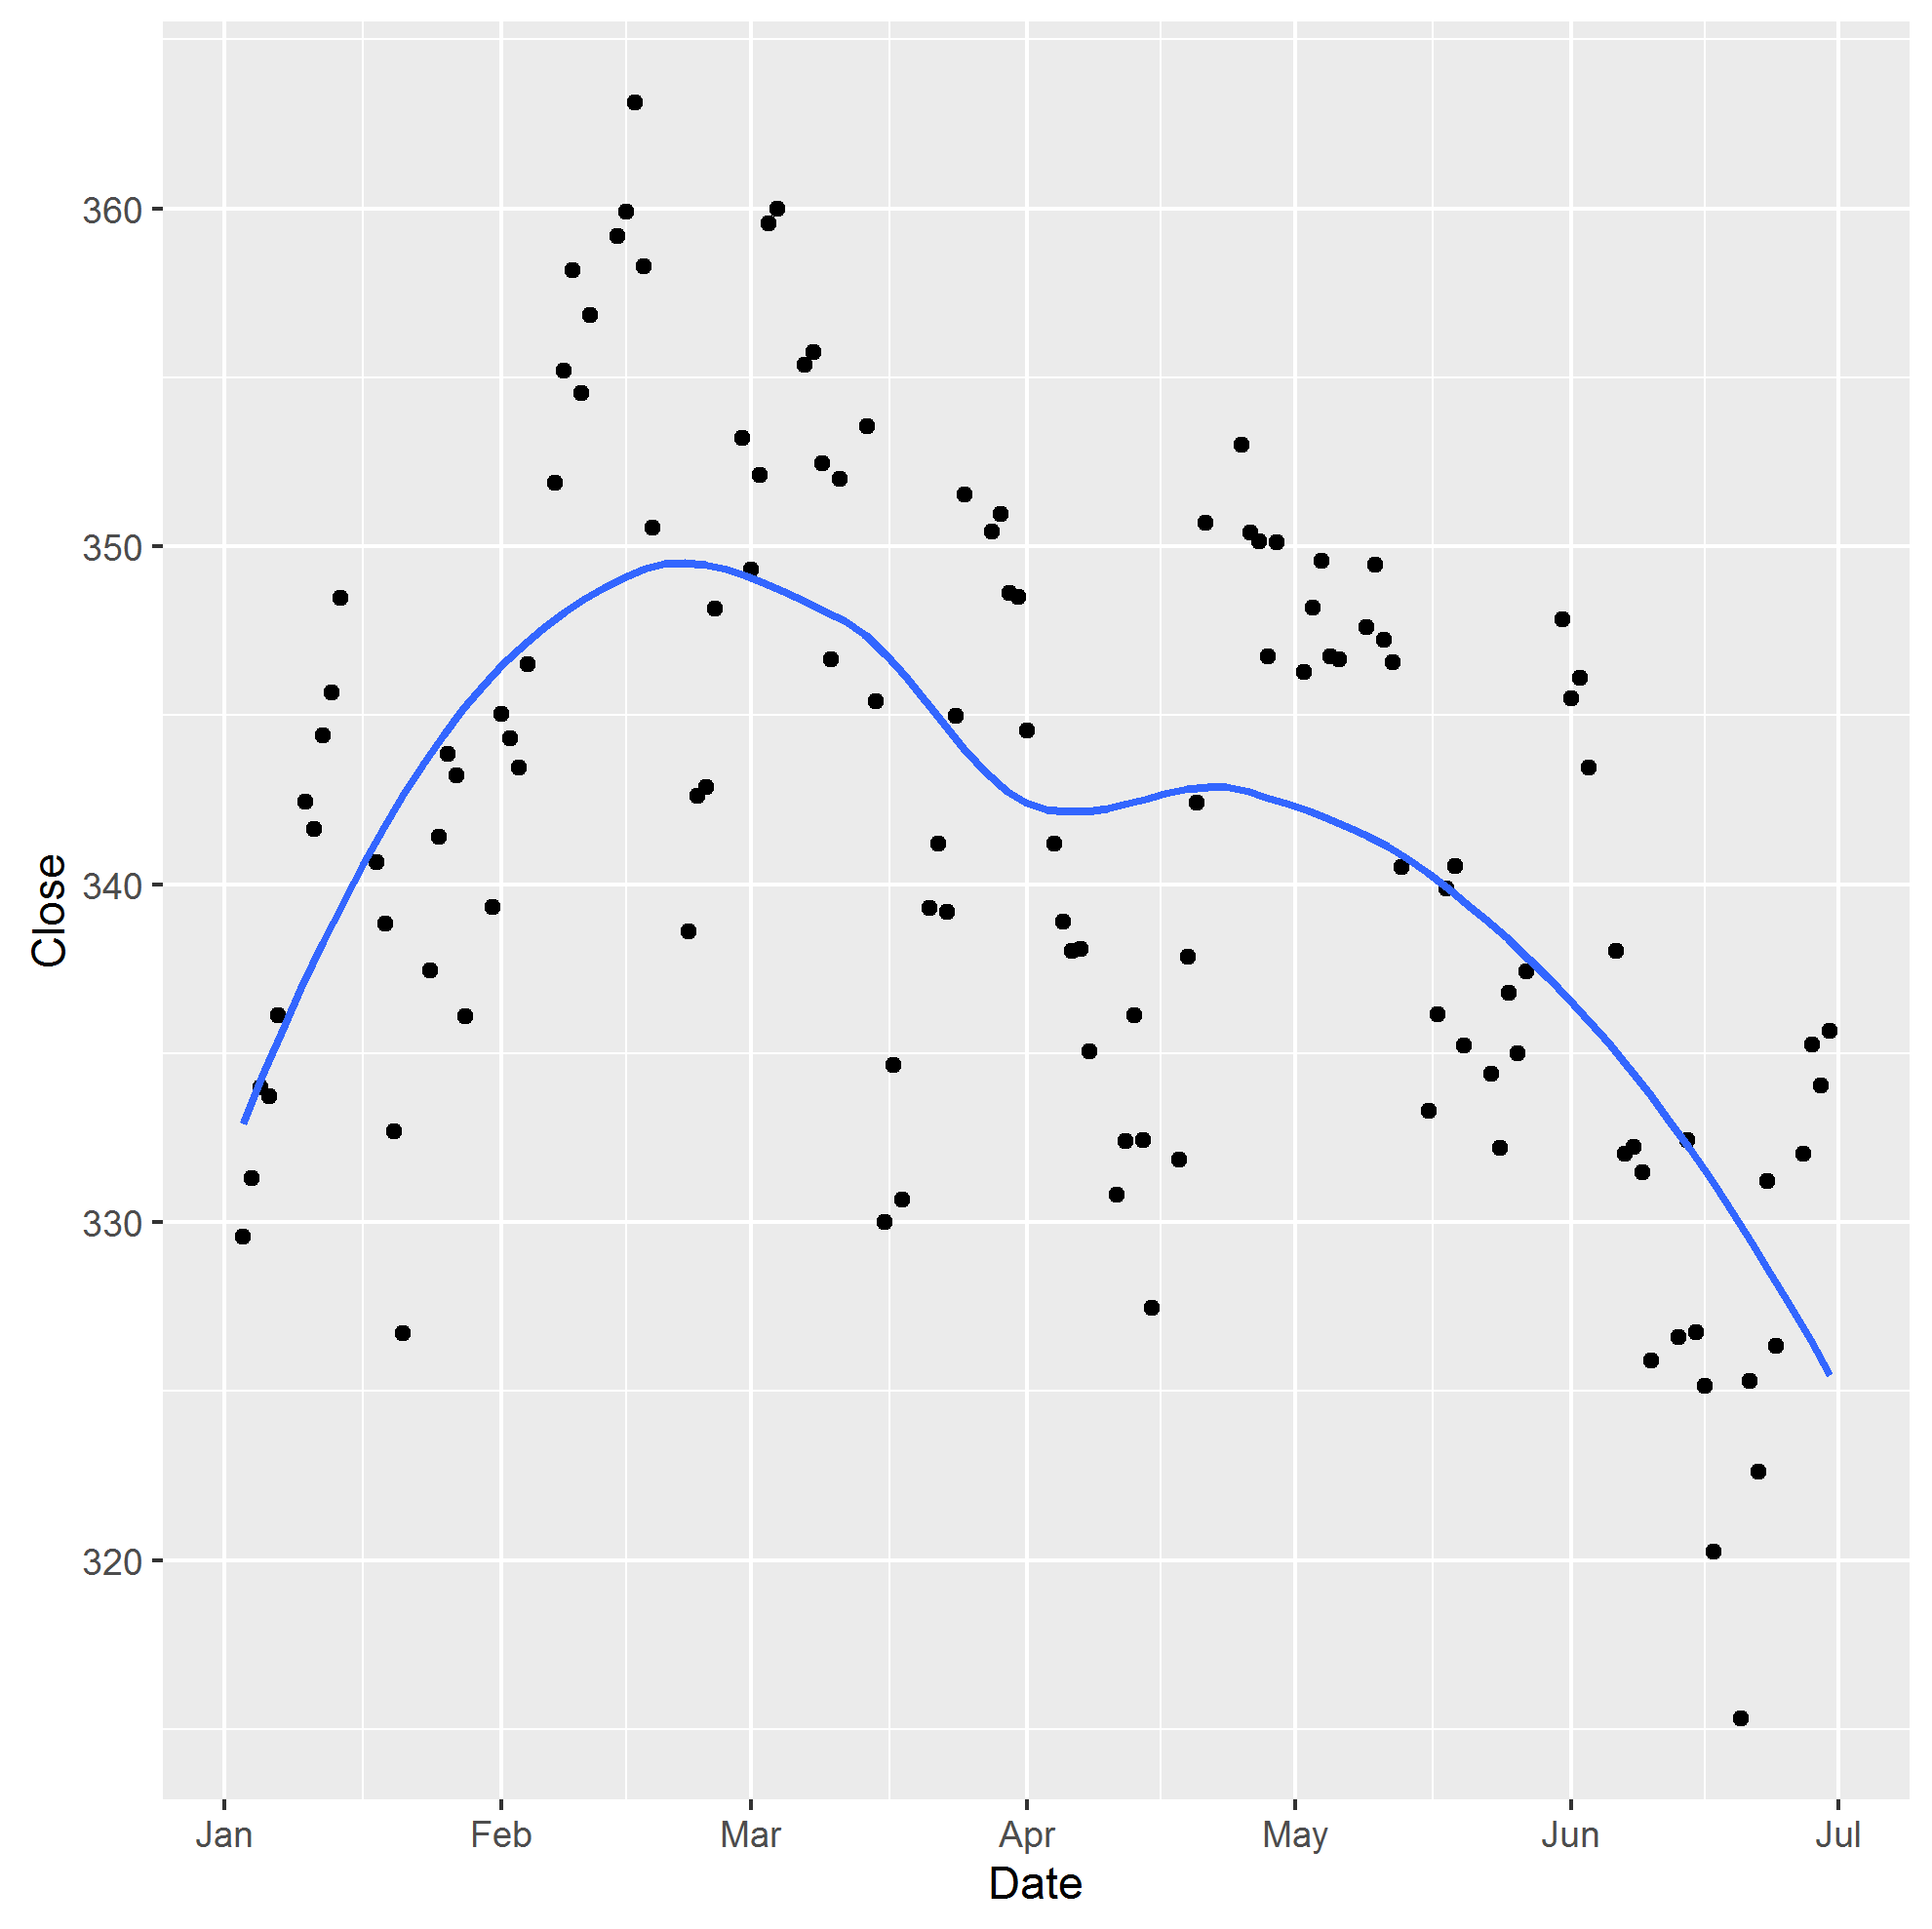
\includegraphics[width=\linewidth]{graph/AAPL1.png}
  \caption{Scatter plot with graph of Apple stock}
\endminipage\hfill
\minipage{0.46\textwidth}
  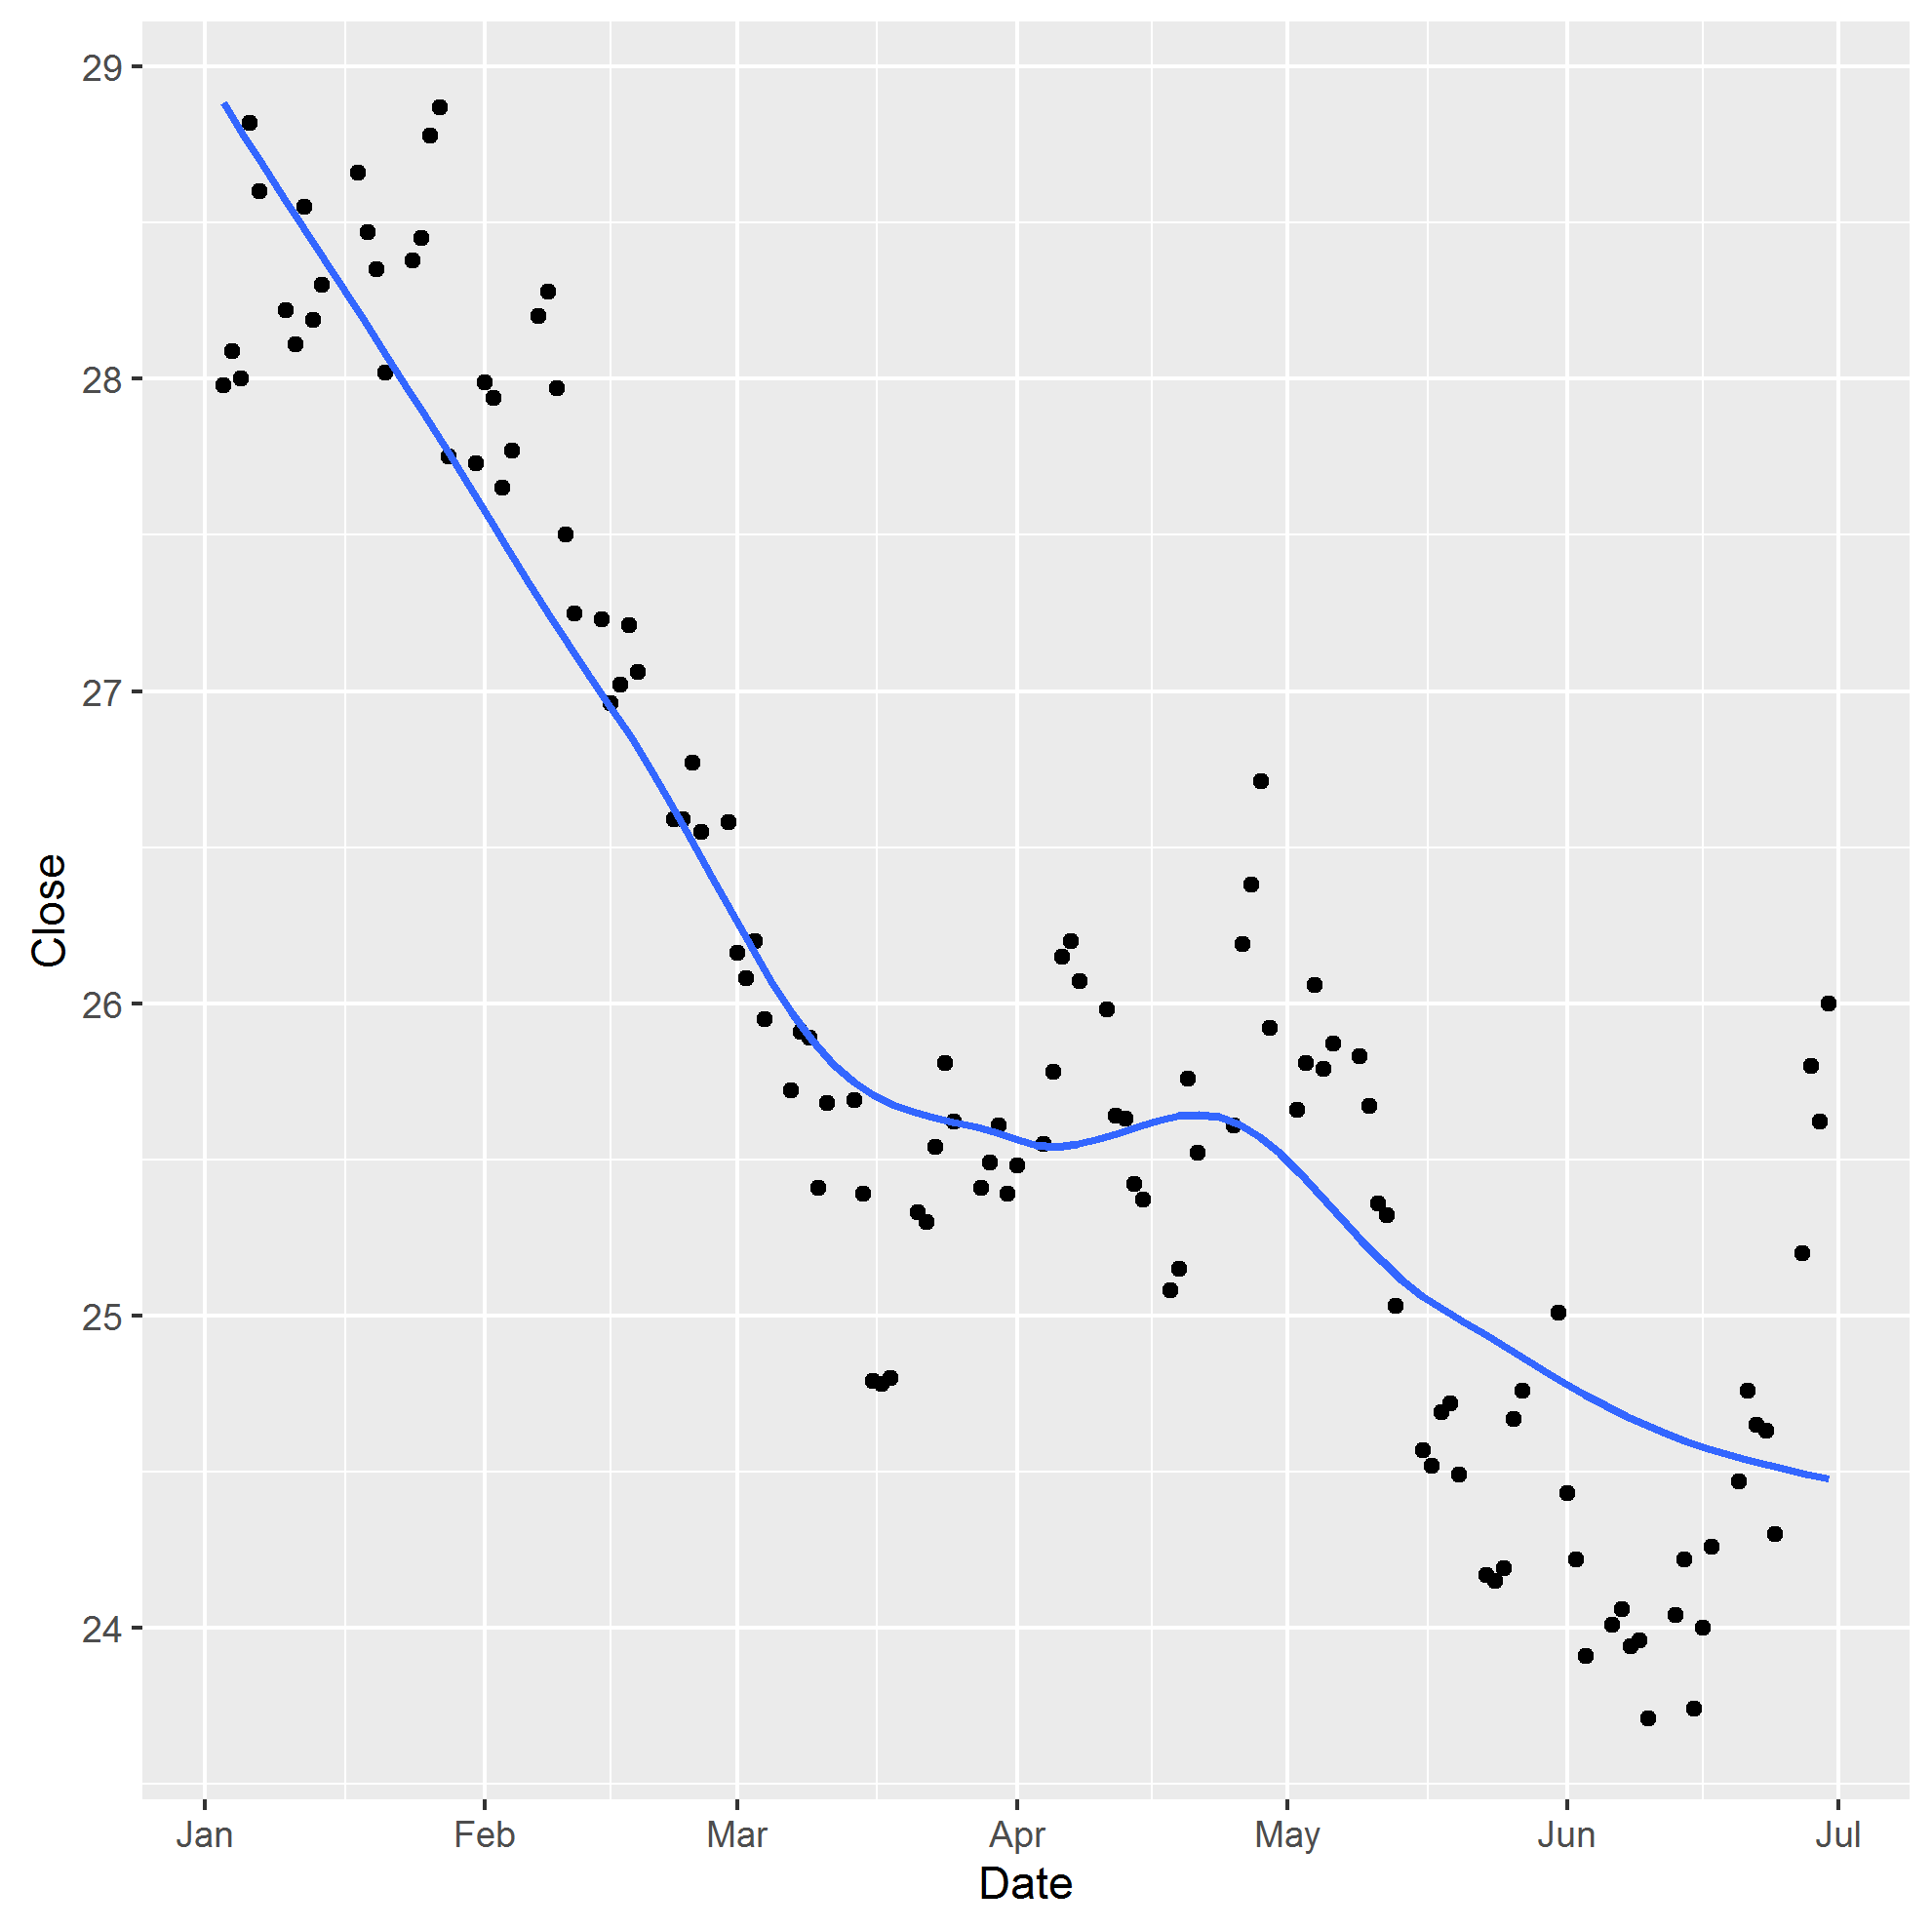
\includegraphics[width=\linewidth]{graph/MSFT1.png}
  \caption{Scatter plot with graph of Microsoft stock}
\endminipage\hfill

\end{figure}
Discuss apple chart
Discuss Microsoft chart
\subsubsection{Correlation}

\begin{figure}[!htb]
\minipage{0.8\textwidth}
  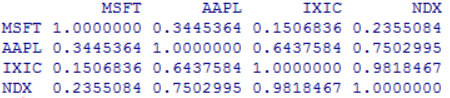
\includegraphics[width=\linewidth]{graph/cor1.png}
  \caption{Correlation table for Microsoft and Apple against two index stocks}
\endminipage\hfill
\end{figure}

Insert correlation table MS vs apple
Discuss any interesting overall observations here

\subsubsection{Regression}
Show regression lines for MS and apple. 


\begin{figure}[!htb]
\minipage{0.46\textwidth}
  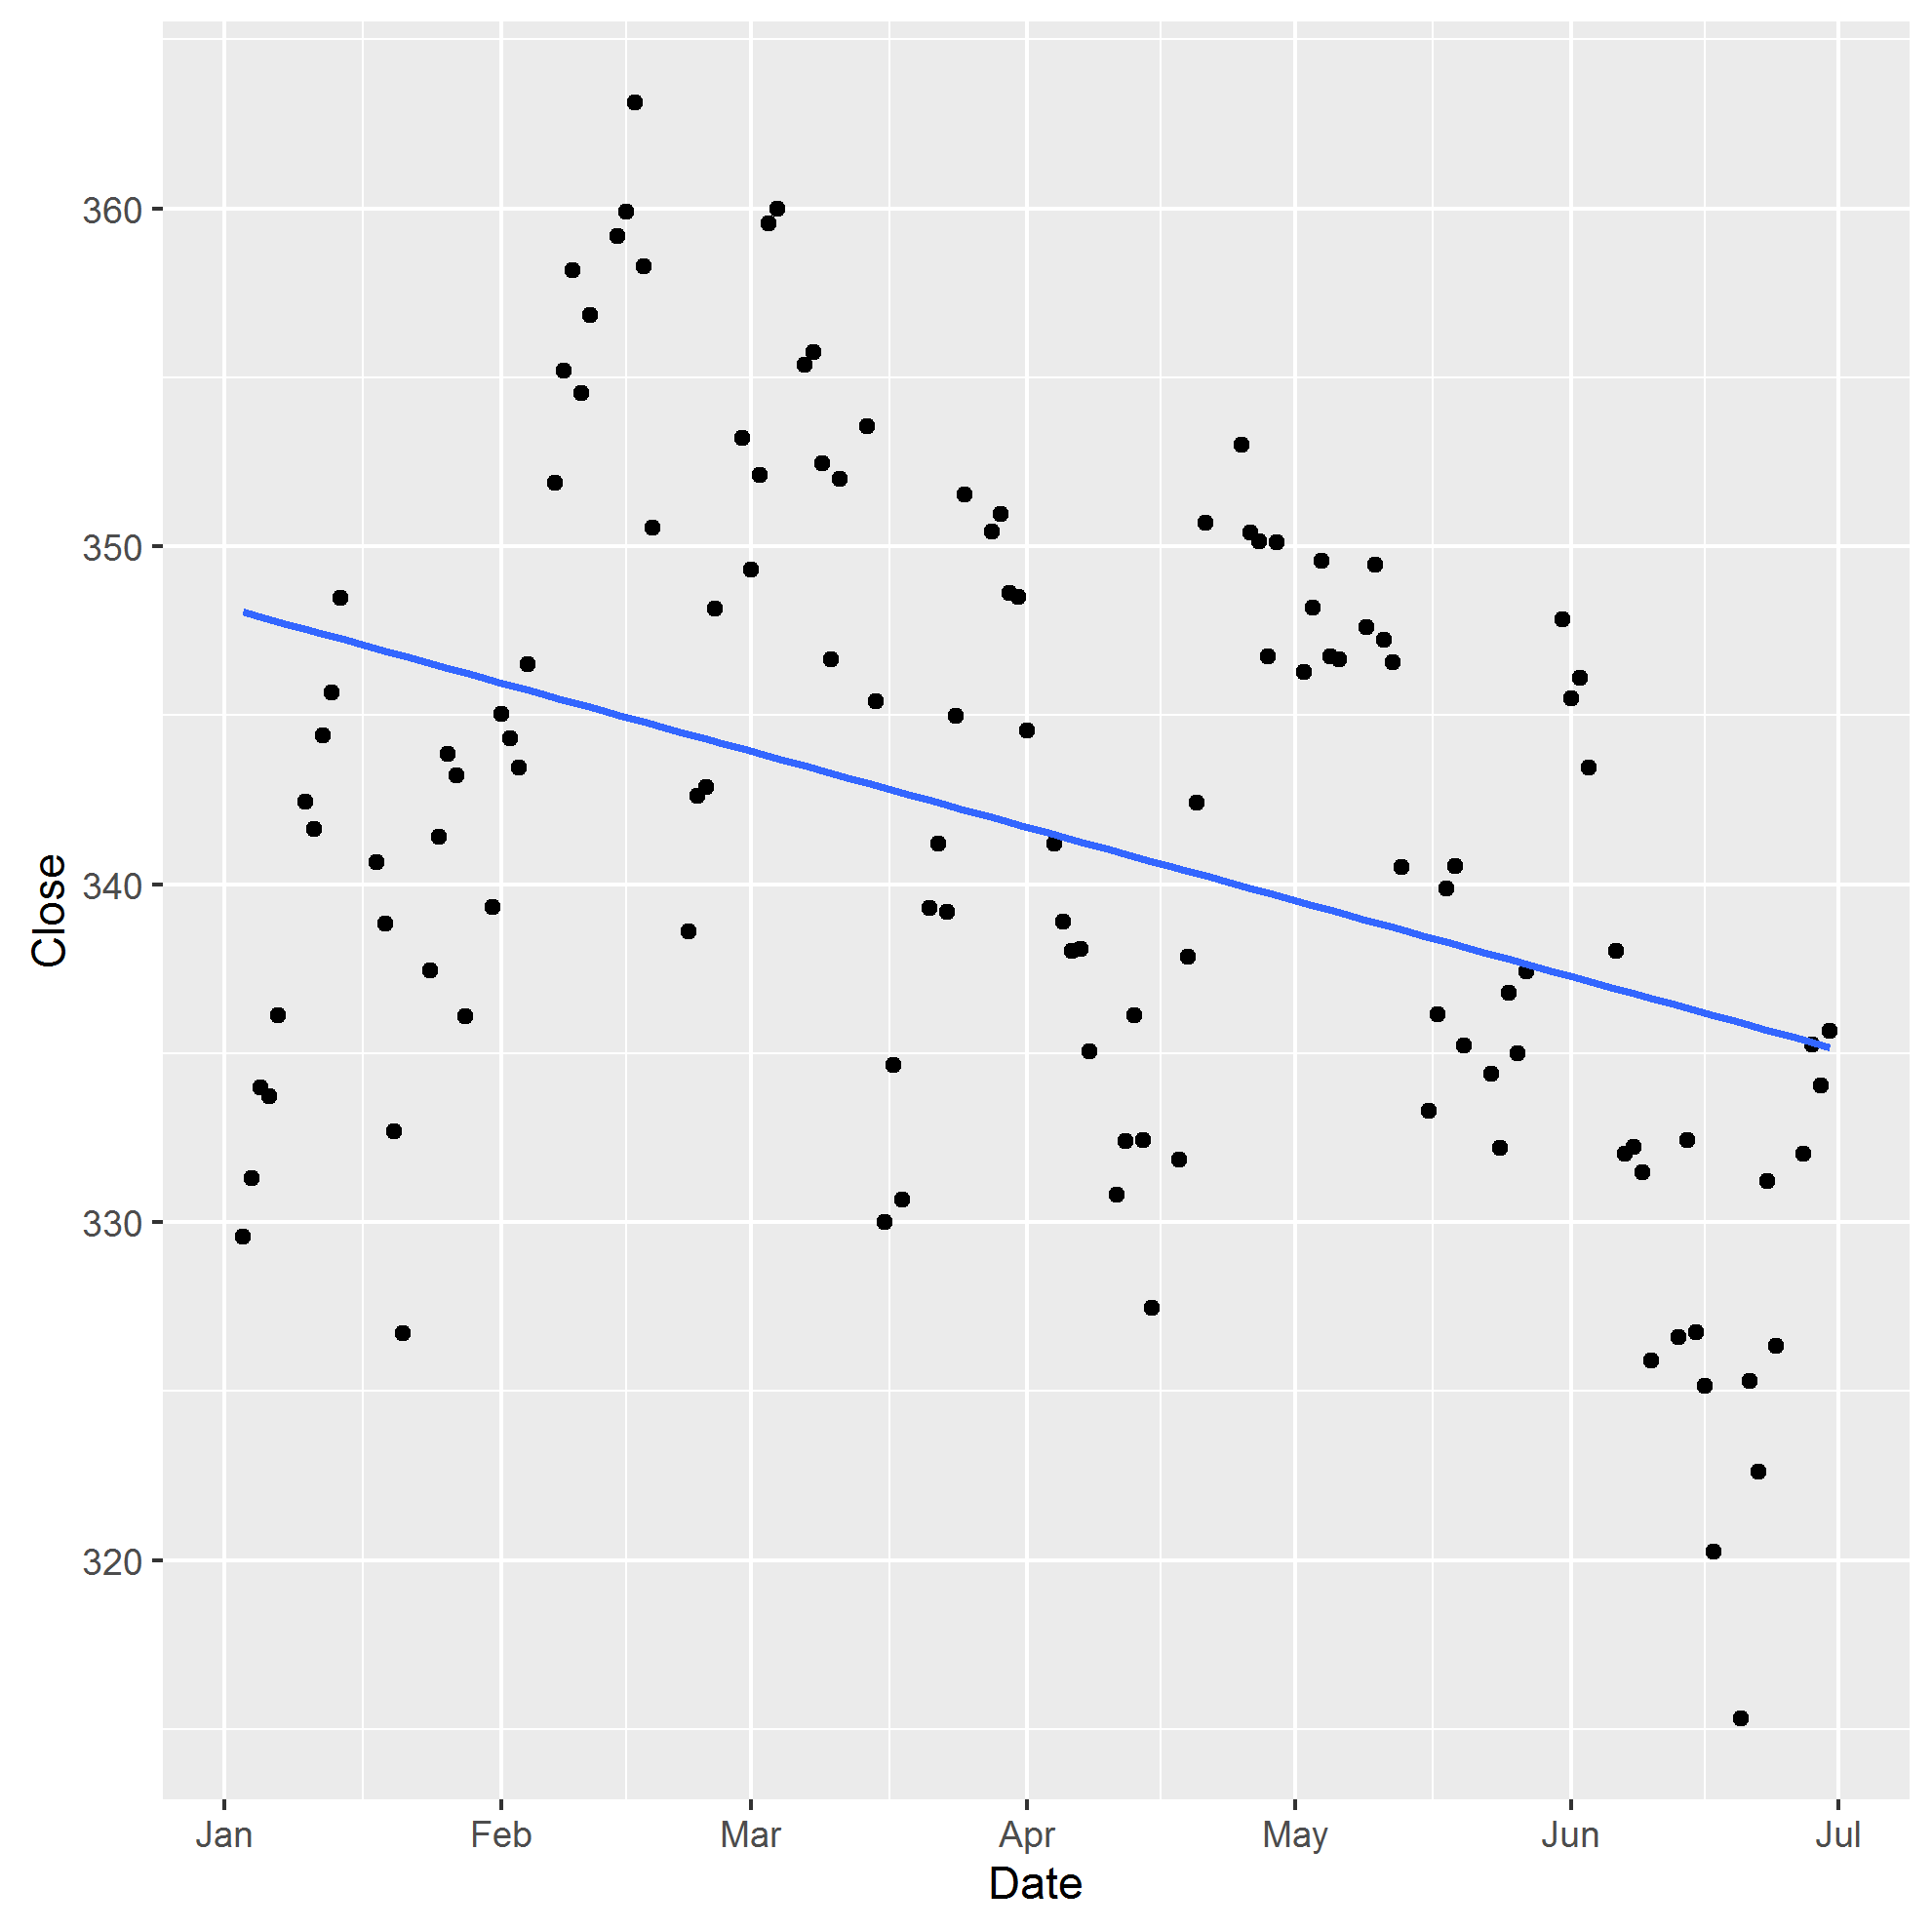
\includegraphics[width=\linewidth]{graph/a_reg1.png}
  \caption{Linear regression line of Apple closing prices.}
\endminipage\hfill
\minipage{0.46\textwidth}
  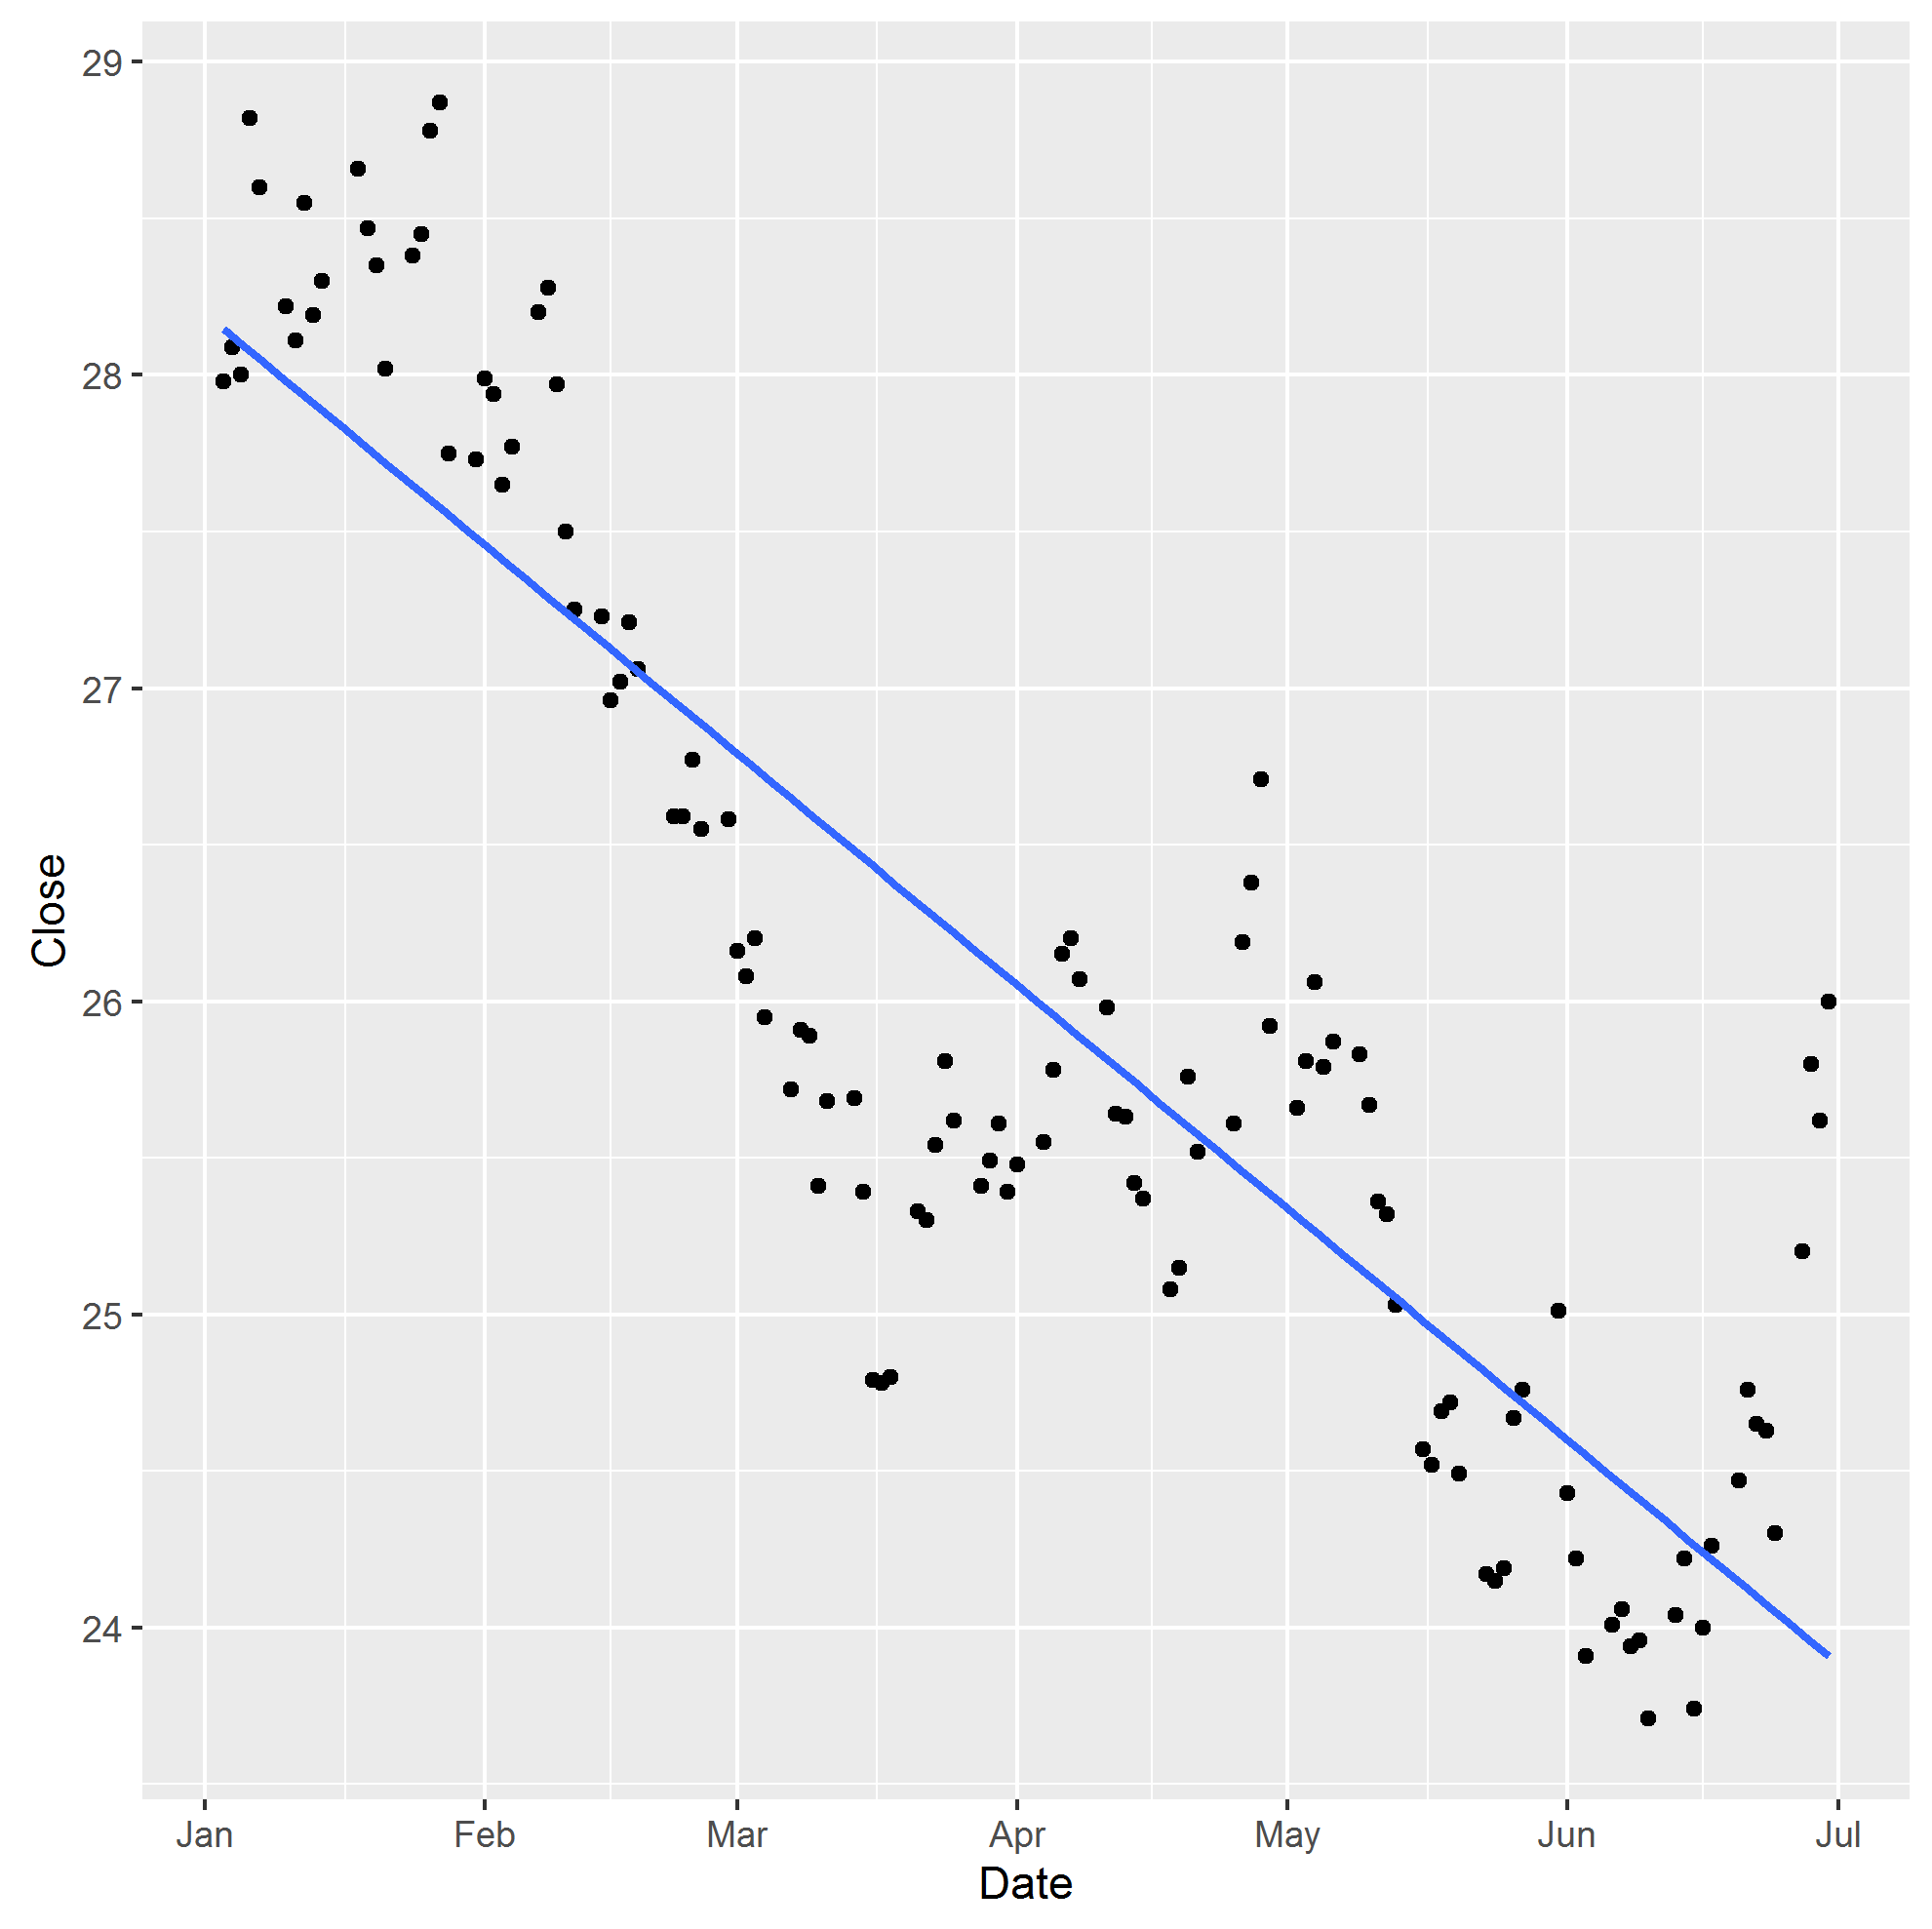
\includegraphics[width=\linewidth]{graph/m_reg1.png}
  \caption{Linear regression line of Microsoft closing prices.}
\endminipage\hfill
\end{figure}

Discuss regression lines. 

List y intercept, slope overall. 

\begin{figure}[!htb]
\minipage{0.46\textwidth}
  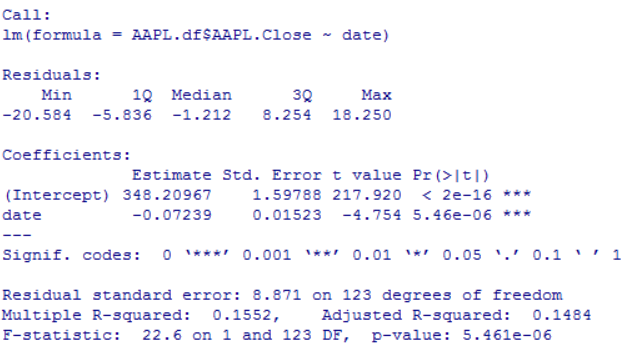
\includegraphics[width=\linewidth]{graph/aapl_reg_1.png}
  \caption{Linear regression line of Apple closing prices.}
\endminipage\hfill
\minipage{0.46\textwidth}
  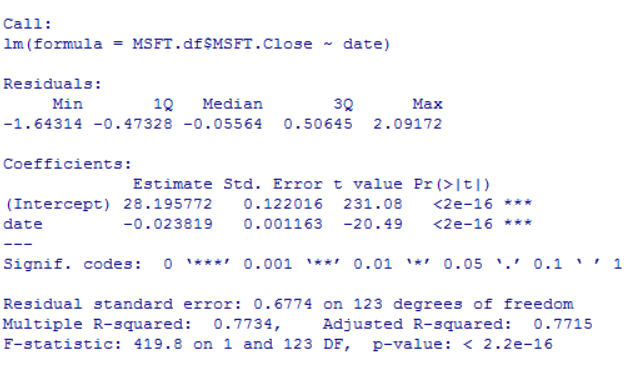
\includegraphics[width=\linewidth]{graph/msft_reg_1.png}
  \caption{Linear regression line of Microsoft closing prices.}
\endminipage\hfill
\end{figure}


\subsubsection{Analysis}
Discuss any interesting overall observations here

\subsection{July - December  2011 }
\subsubsection{Plots}
\begin{figure}[!htb]
\minipage{0.46\textwidth}
  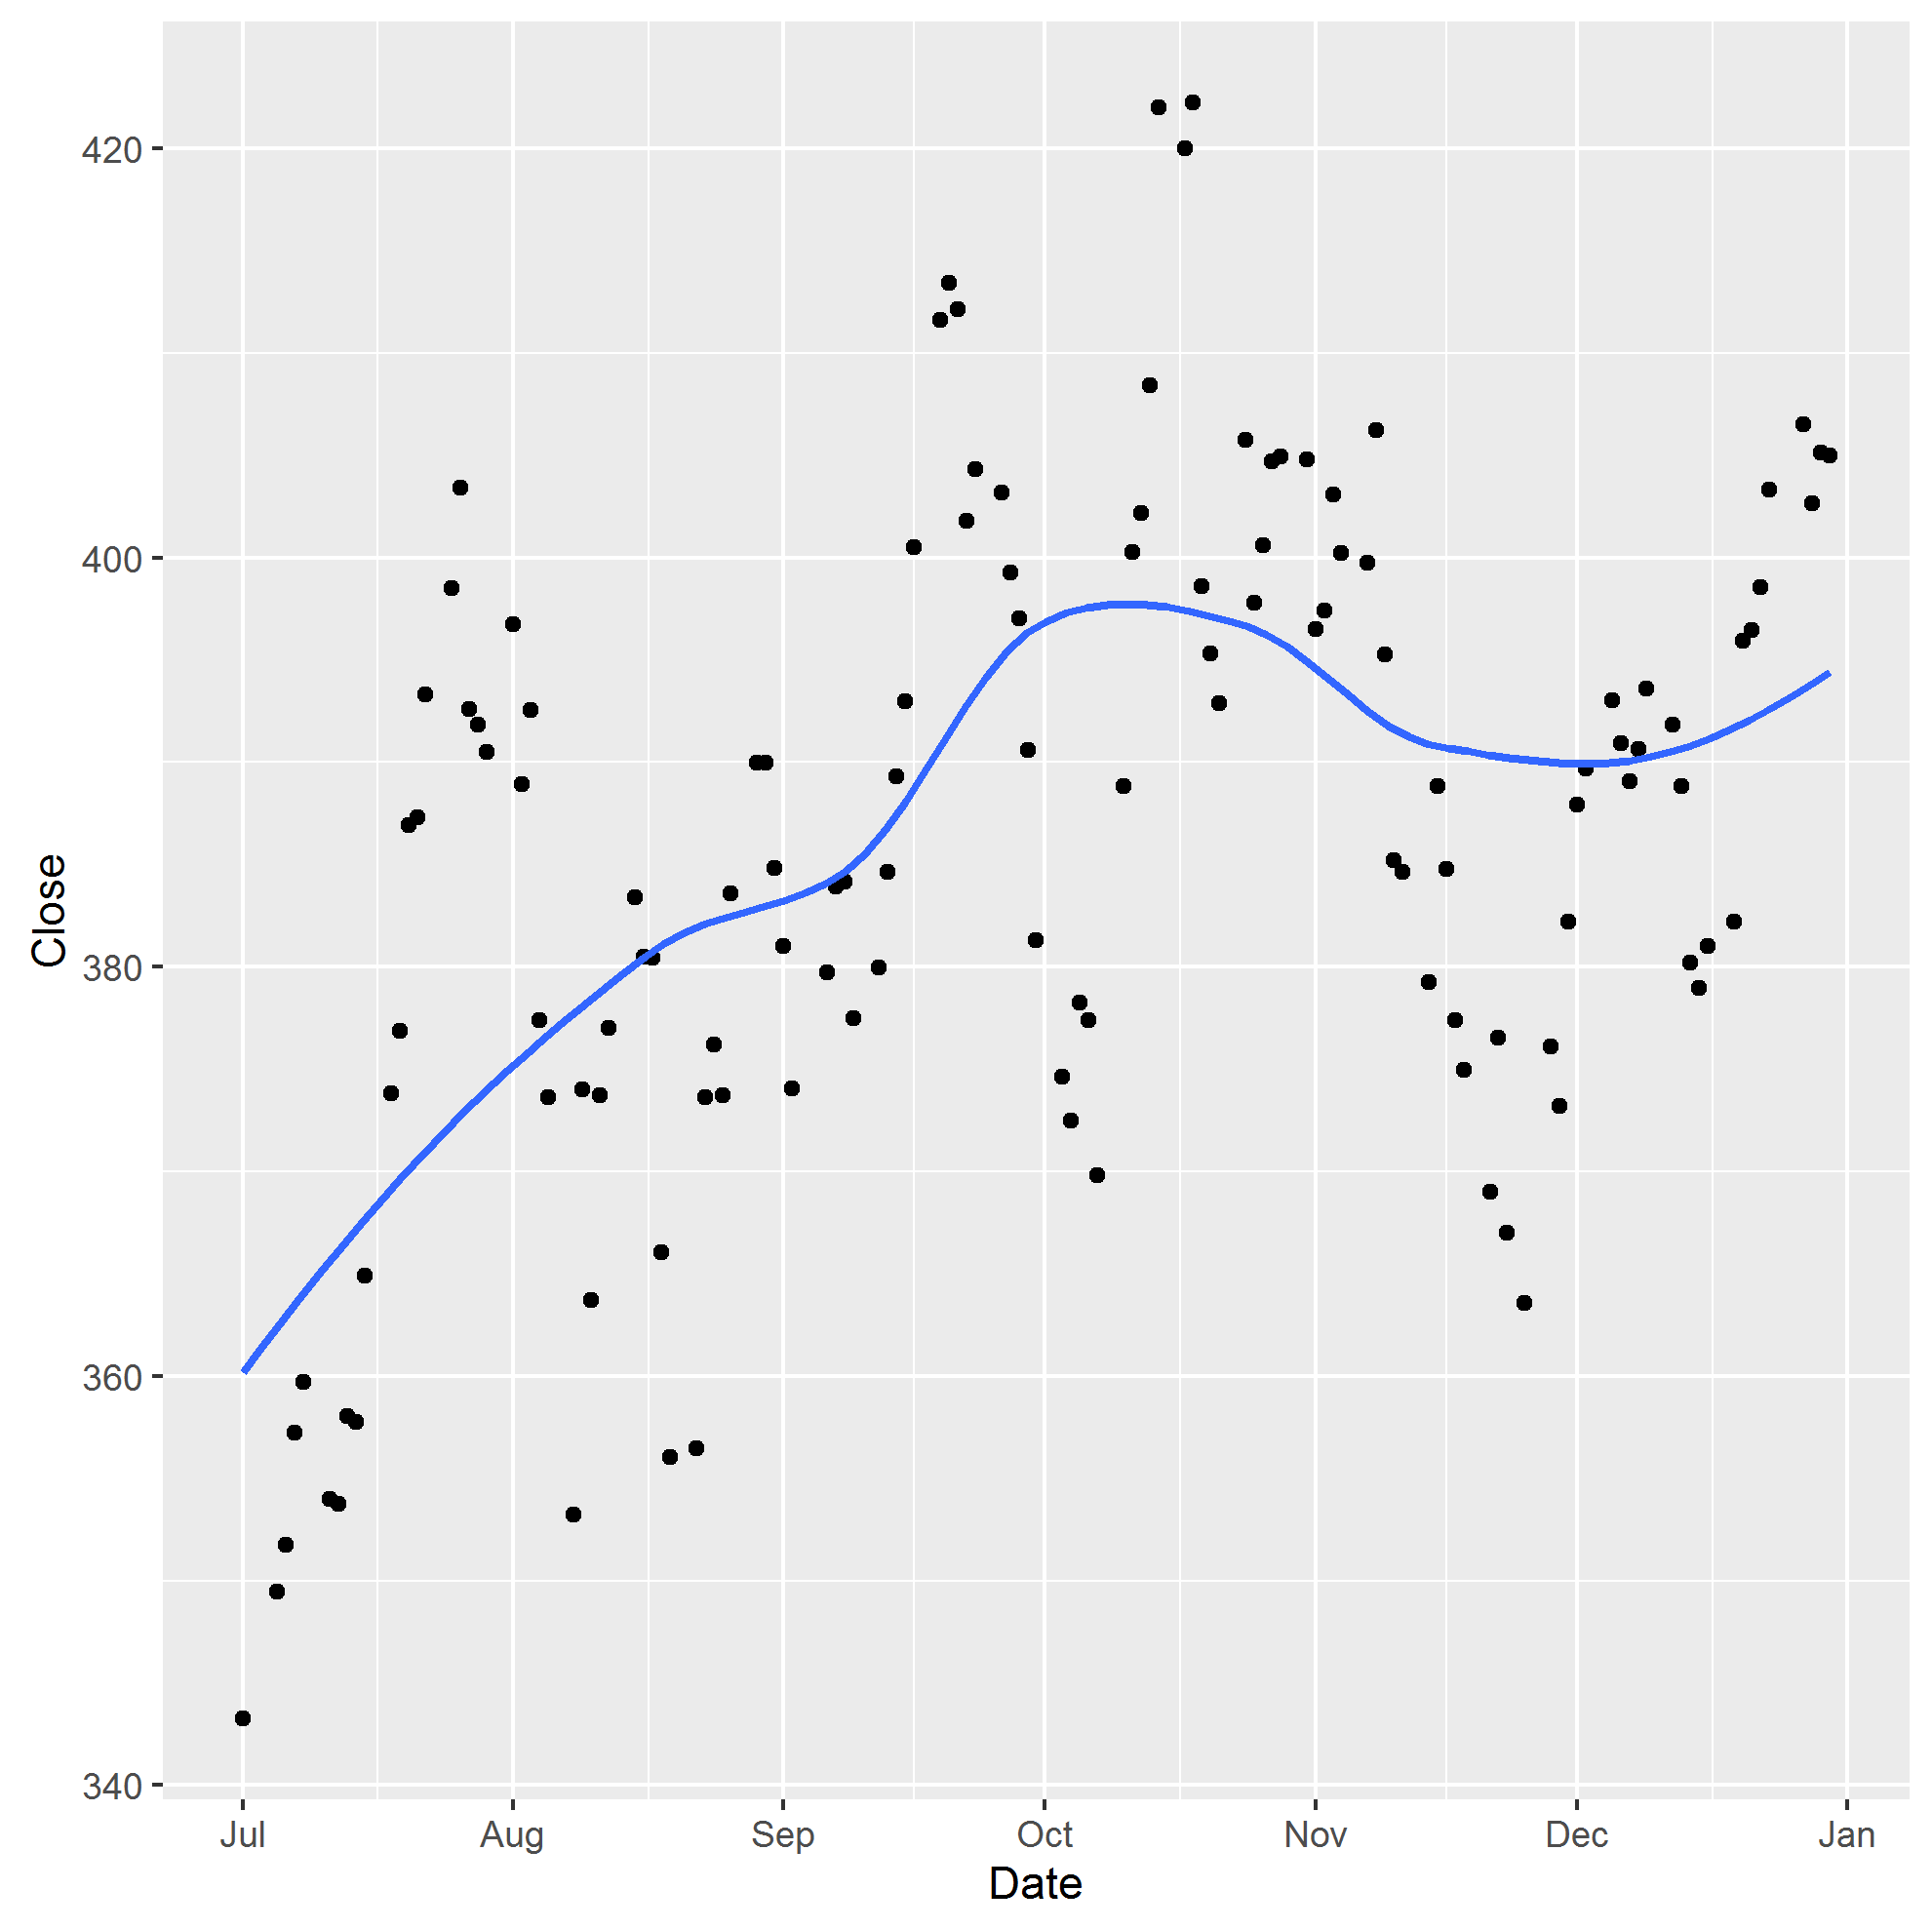
\includegraphics[width=\linewidth]{graph/AAPL2.png}
  \caption{Scatter plot with graph of Apple stock}
\endminipage\hfill
\minipage{0.46\textwidth}
  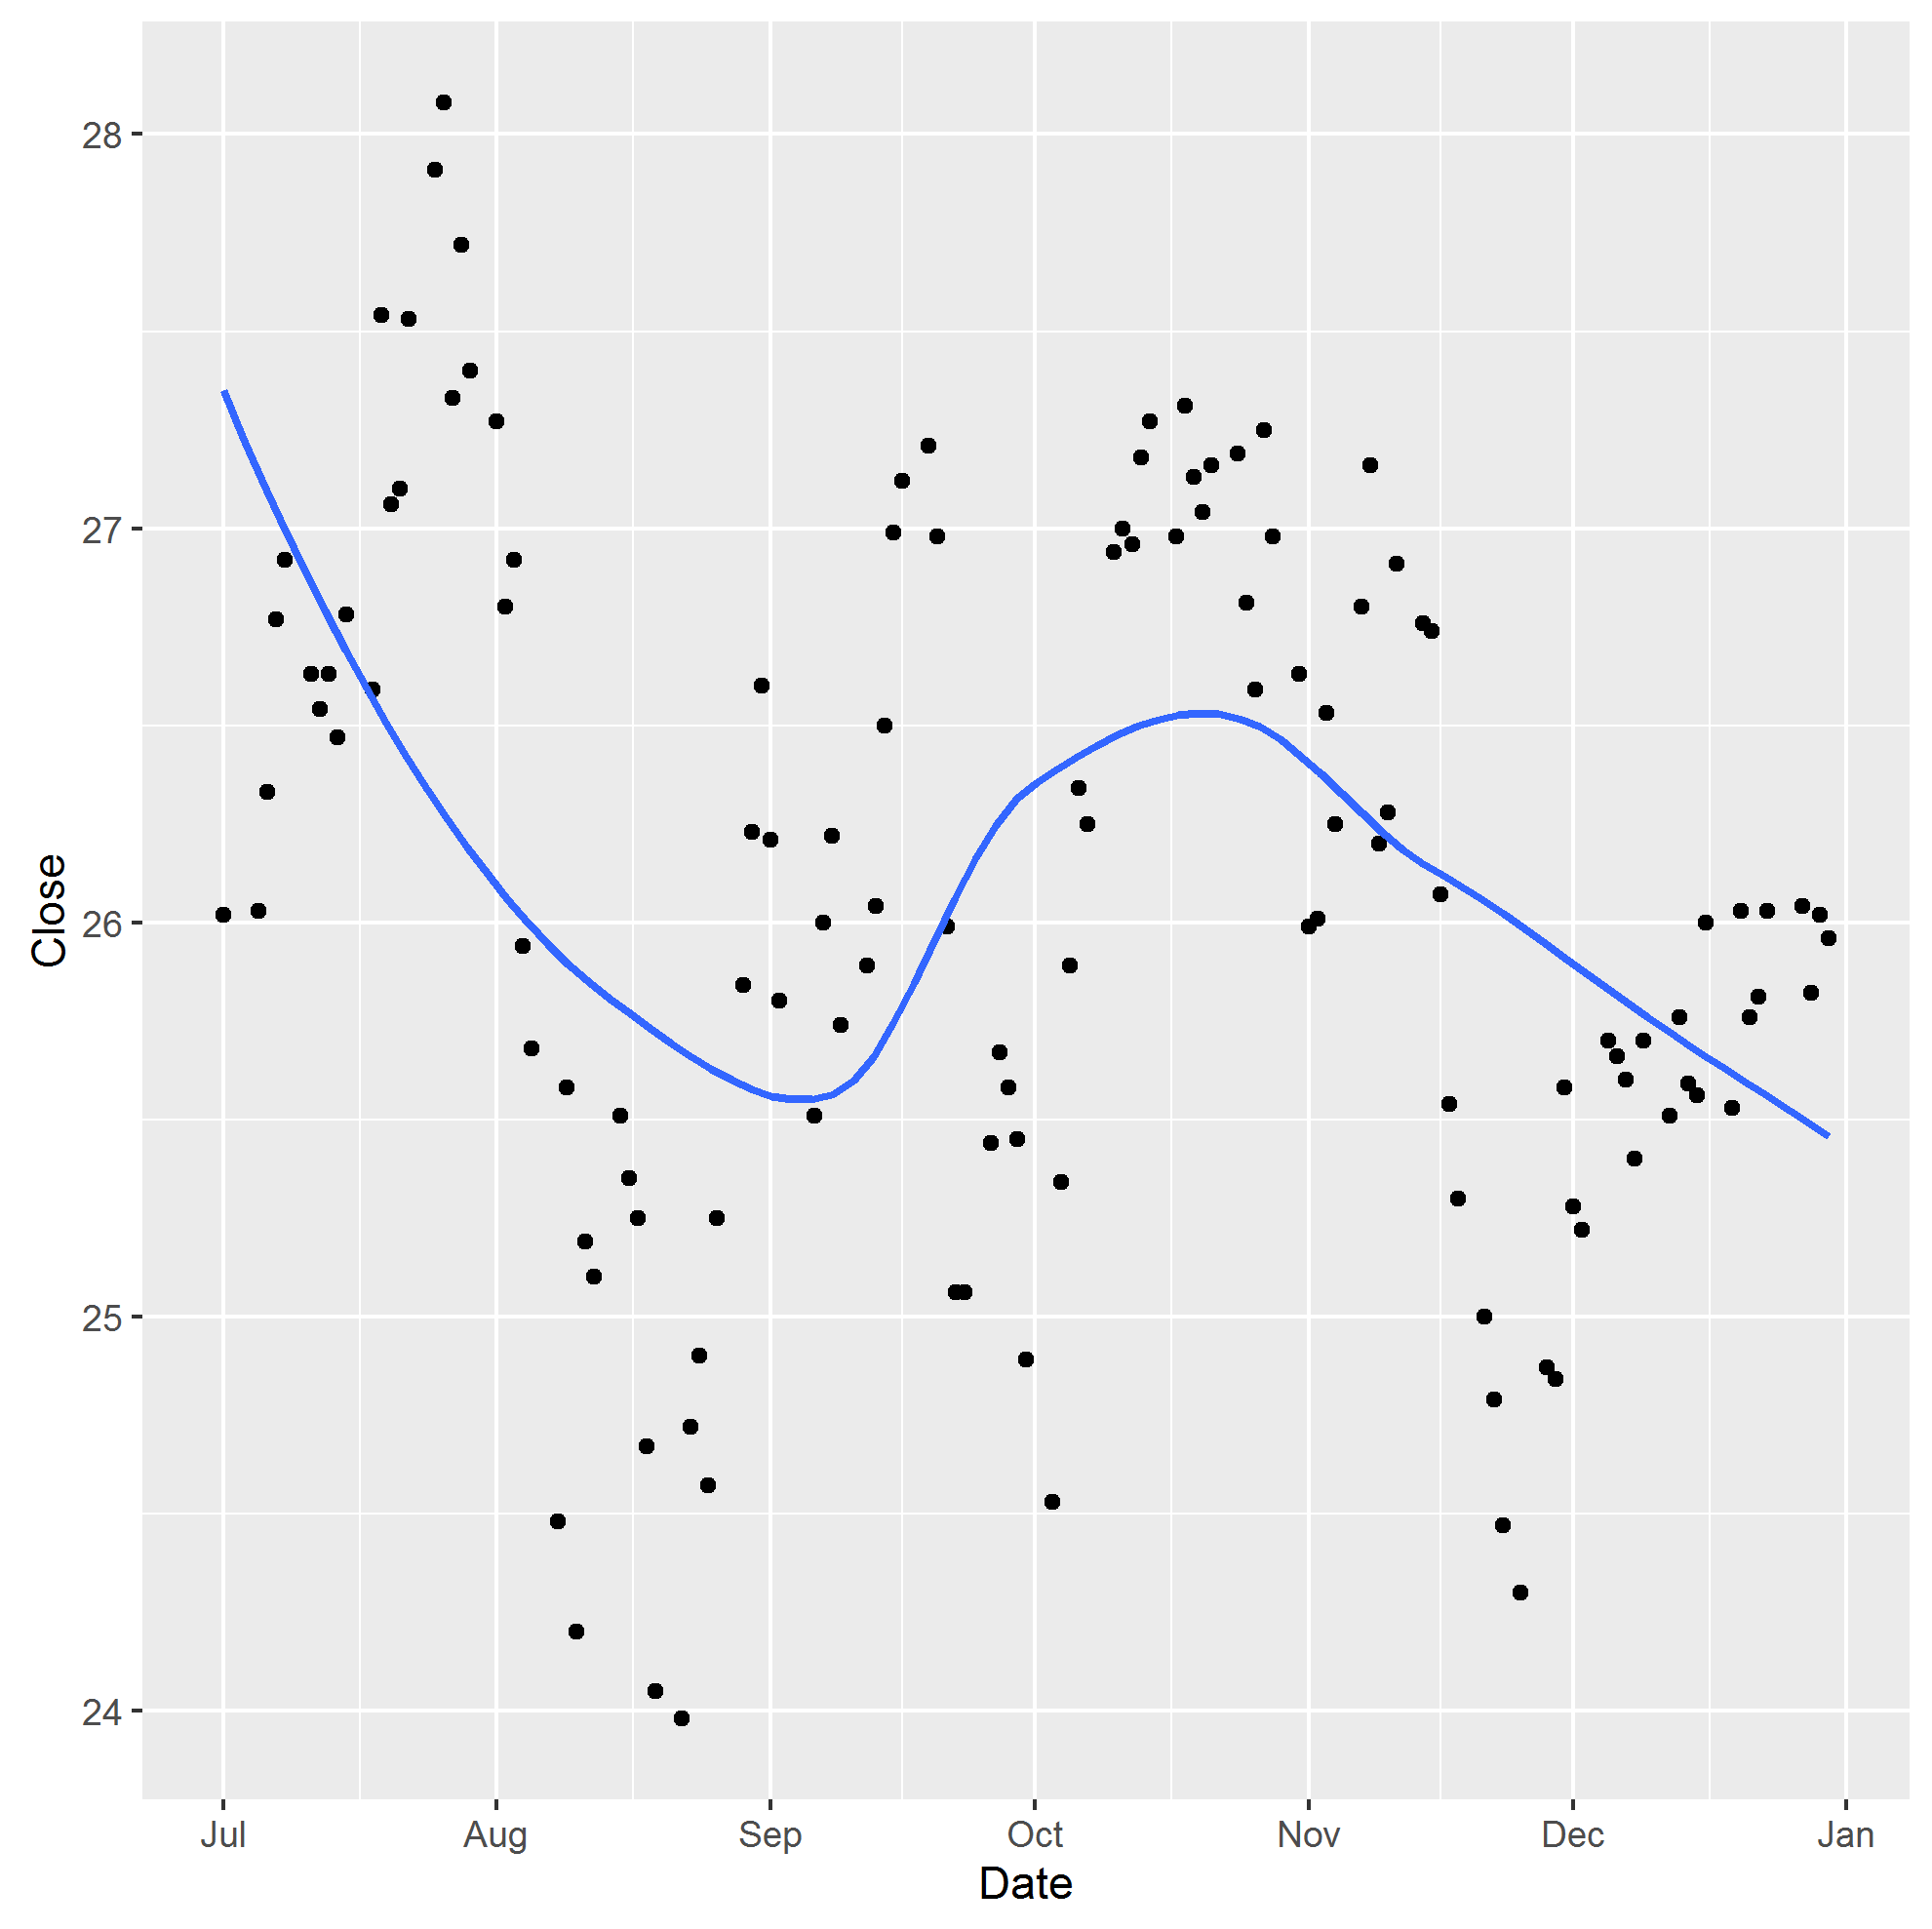
\includegraphics[width=\linewidth]{graph/MSFT2.png}
  \caption{Scatter plot with graph of Microsoft stock}
\endminipage\hfill

\end{figure}
Discuss apple chart
Discuss Microsoft chart
\subsubsection{Correlation}

\begin{figure}[!htb]
\minipage{0.8\textwidth}
  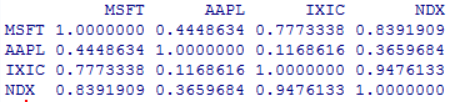
\includegraphics[width=\linewidth]{graph/cor2.png}
  \caption{Correlation table for Microsoft and Apple against two index stocks}
\endminipage\hfill
\end{figure}

Insert correlation table MS vs apple
Discuss any interesting overall observations here

\subsubsection{Regression}
Show regression lines for MS and apple. 


\begin{figure}[!htb]
\minipage{0.46\textwidth}
  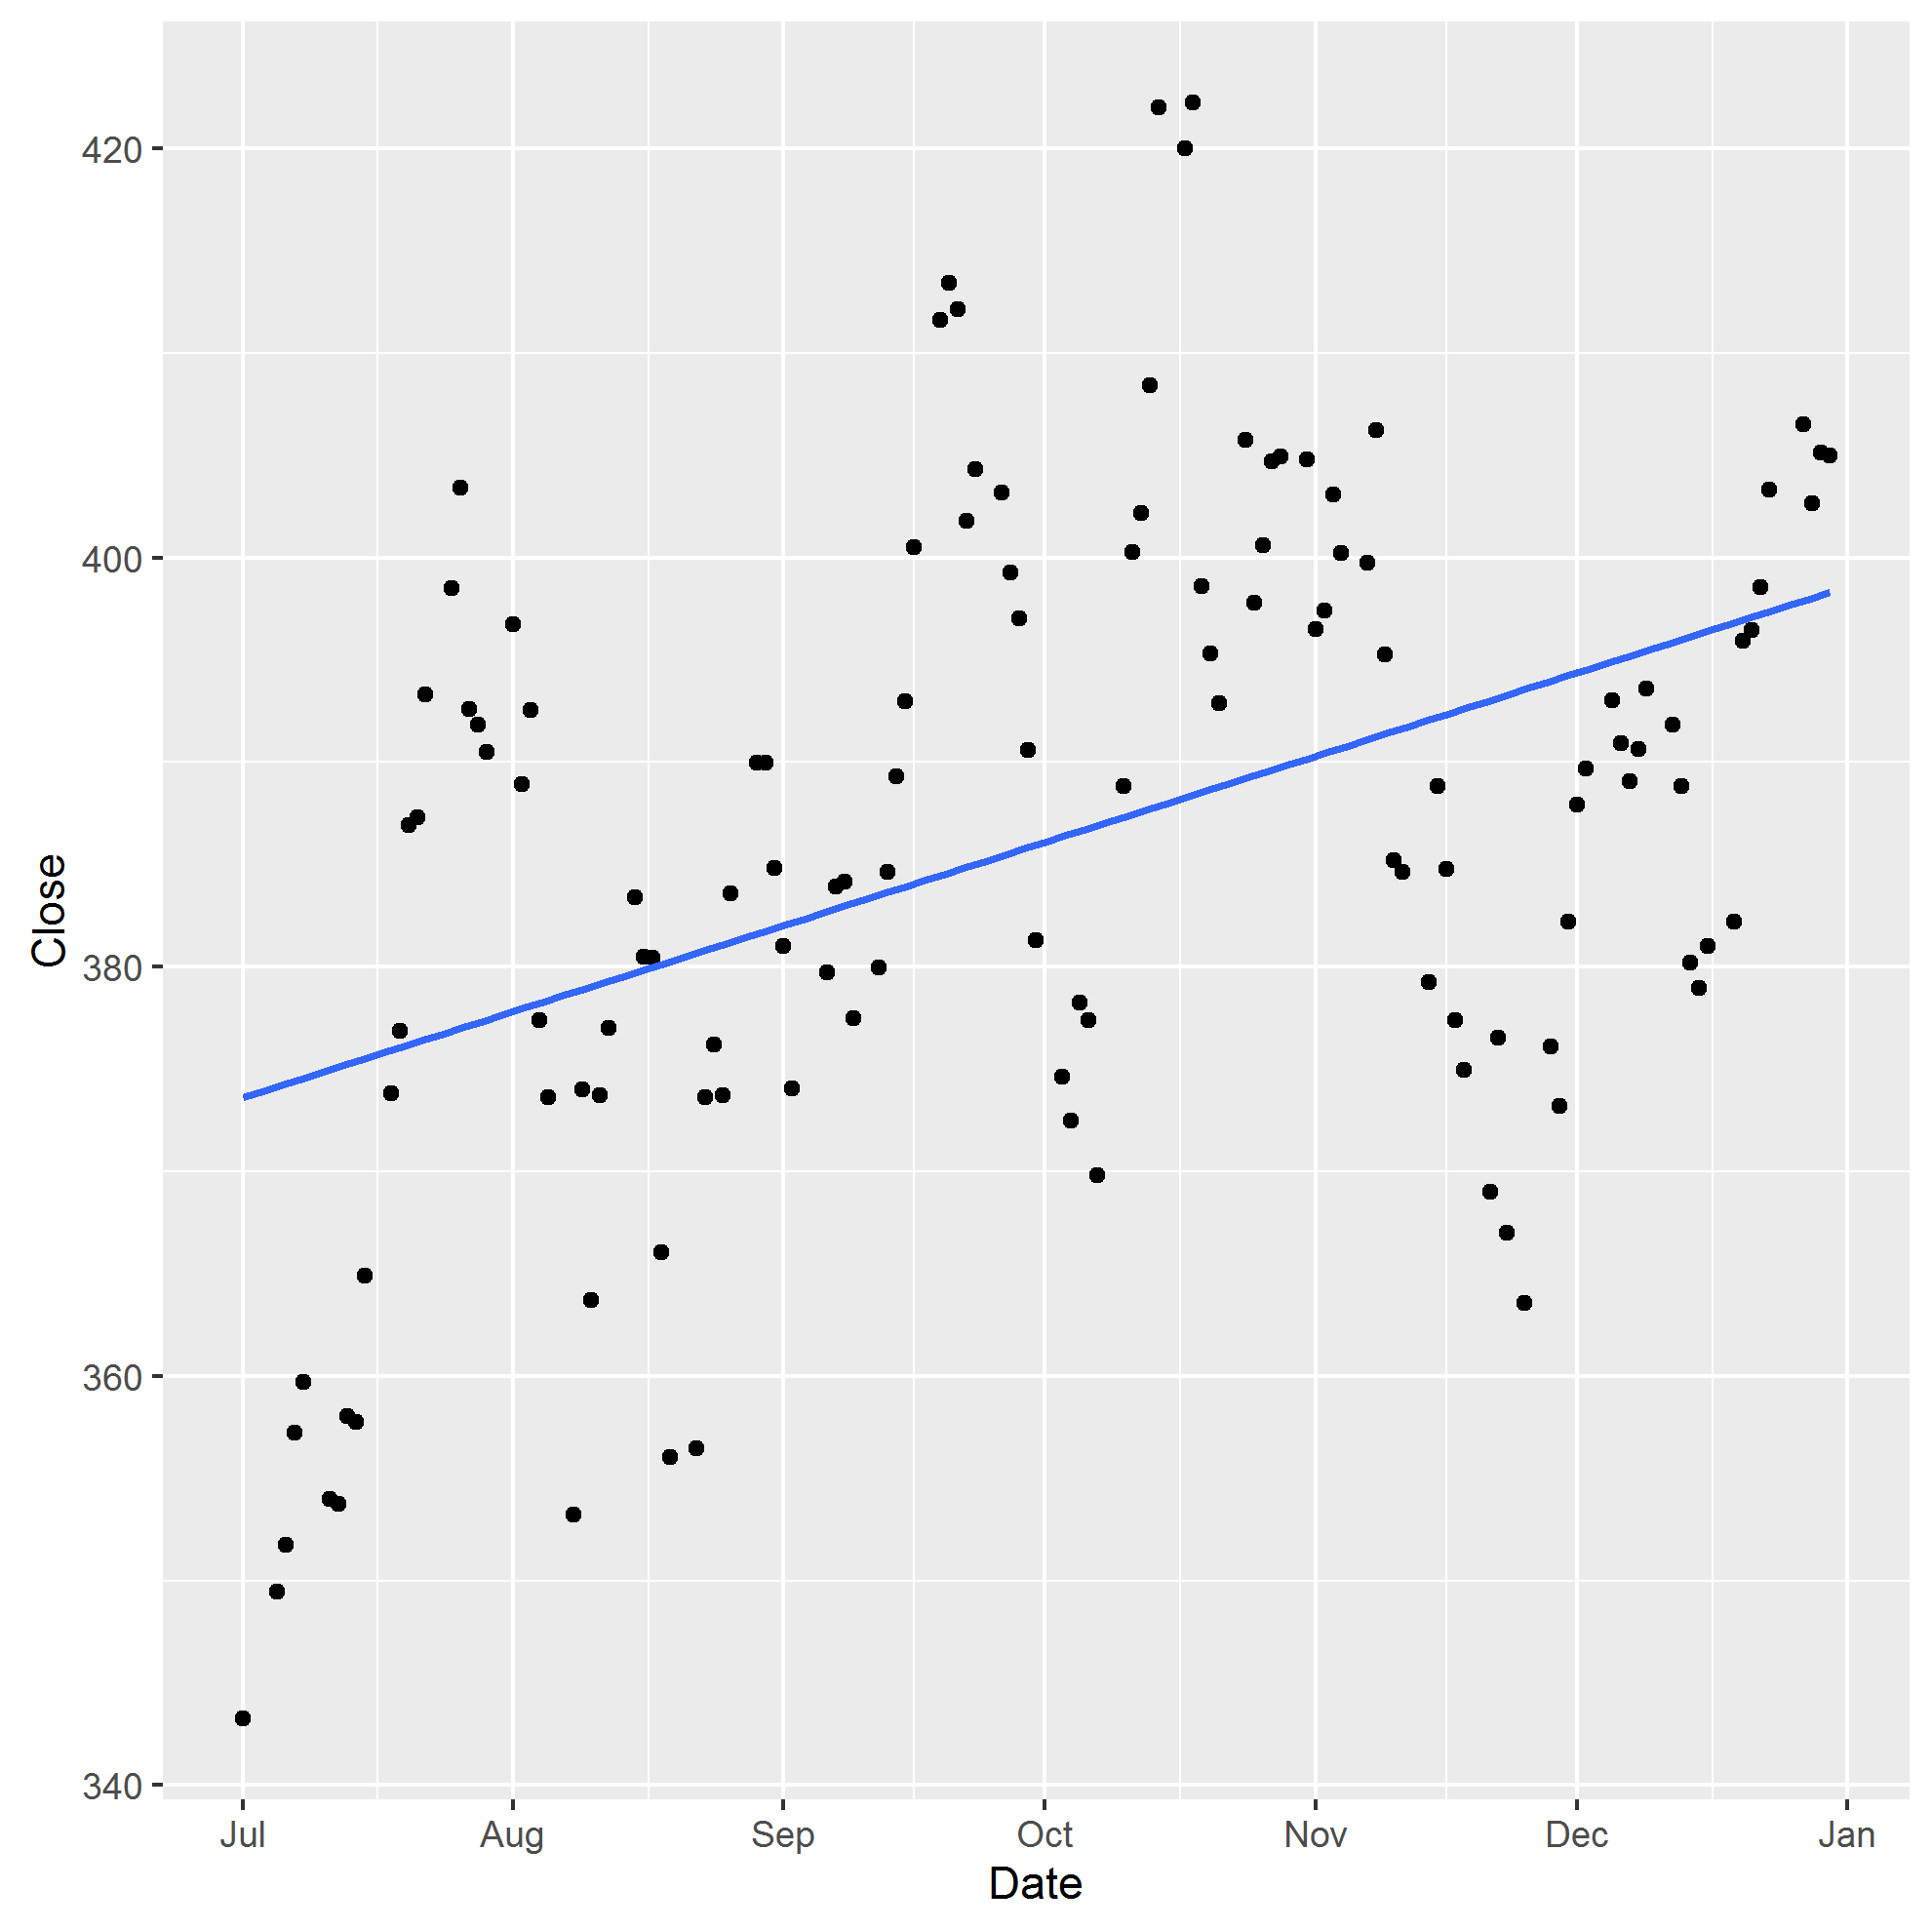
\includegraphics[width=\linewidth]{graph/a_reg2.png}
  \caption{Linear regression line of Apple closing prices.}
\endminipage\hfill
\minipage{0.46\textwidth}
  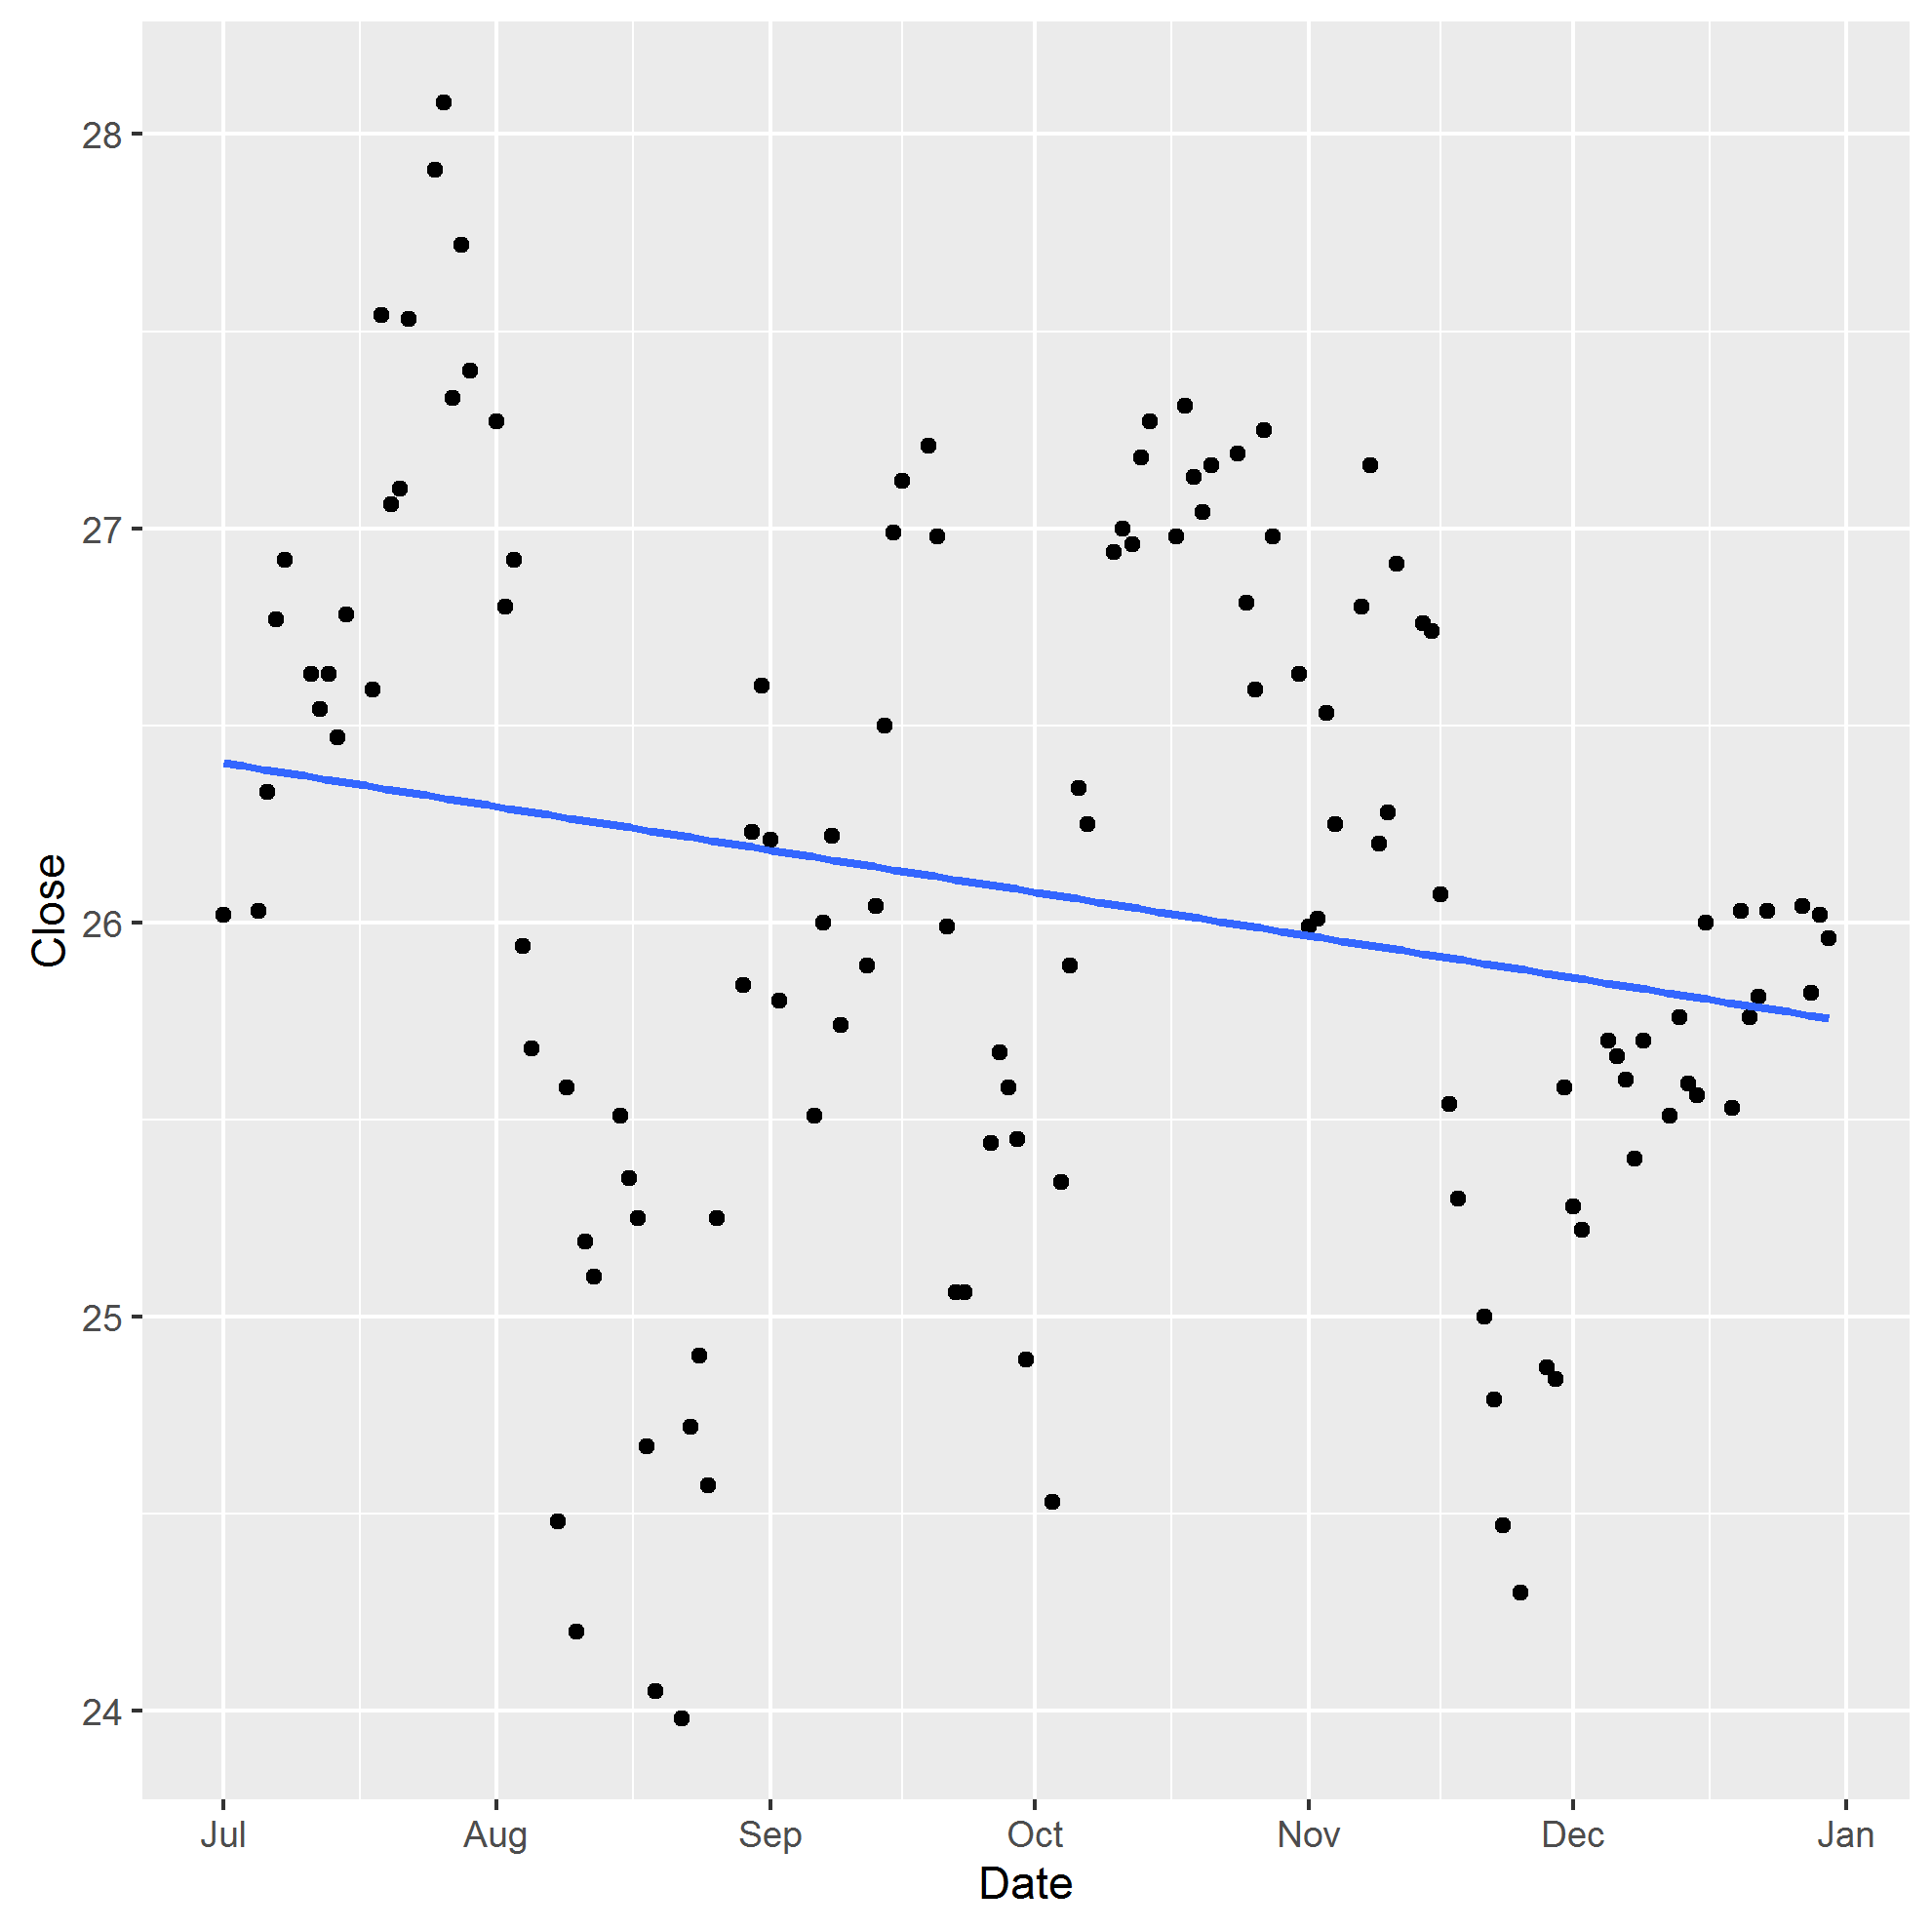
\includegraphics[width=\linewidth]{graph/m_reg2.png}
  \caption{Linear regression line of Microsoft closing prices.}
\endminipage\hfill
\end{figure}

Discuss regression lines. 

List y intercept, slope overall. 

\begin{figure}[!htb]
\minipage{0.46\textwidth}
  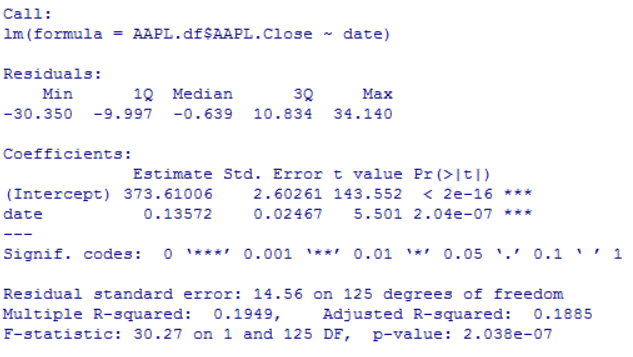
\includegraphics[width=\linewidth]{graph/aapl_reg_2.png}
  \caption{Linear regression line of Apple closing prices.}
\endminipage\hfill
\minipage{0.46\textwidth}
  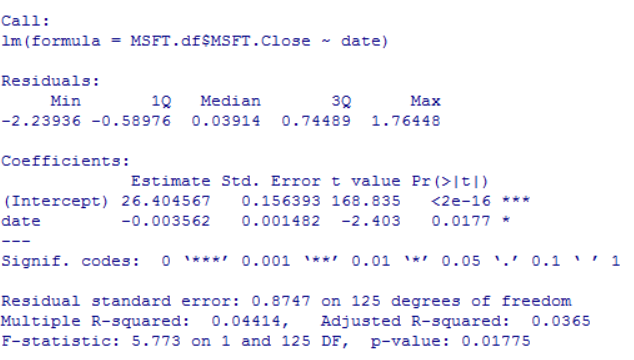
\includegraphics[width=\linewidth]{graph/msft_reg_2.png}
  \caption{Linear regression line of Microsoft closing prices.}
\endminipage\hfill
\end{figure}


\subsubsection{Analysis}
Discuss any interesting overall observations here

Discuss any interesting overall observations here

\subsection{January - June  2012}
\subsubsection{Plots}
\begin{figure}[!htb]
\minipage{0.46\textwidth}
  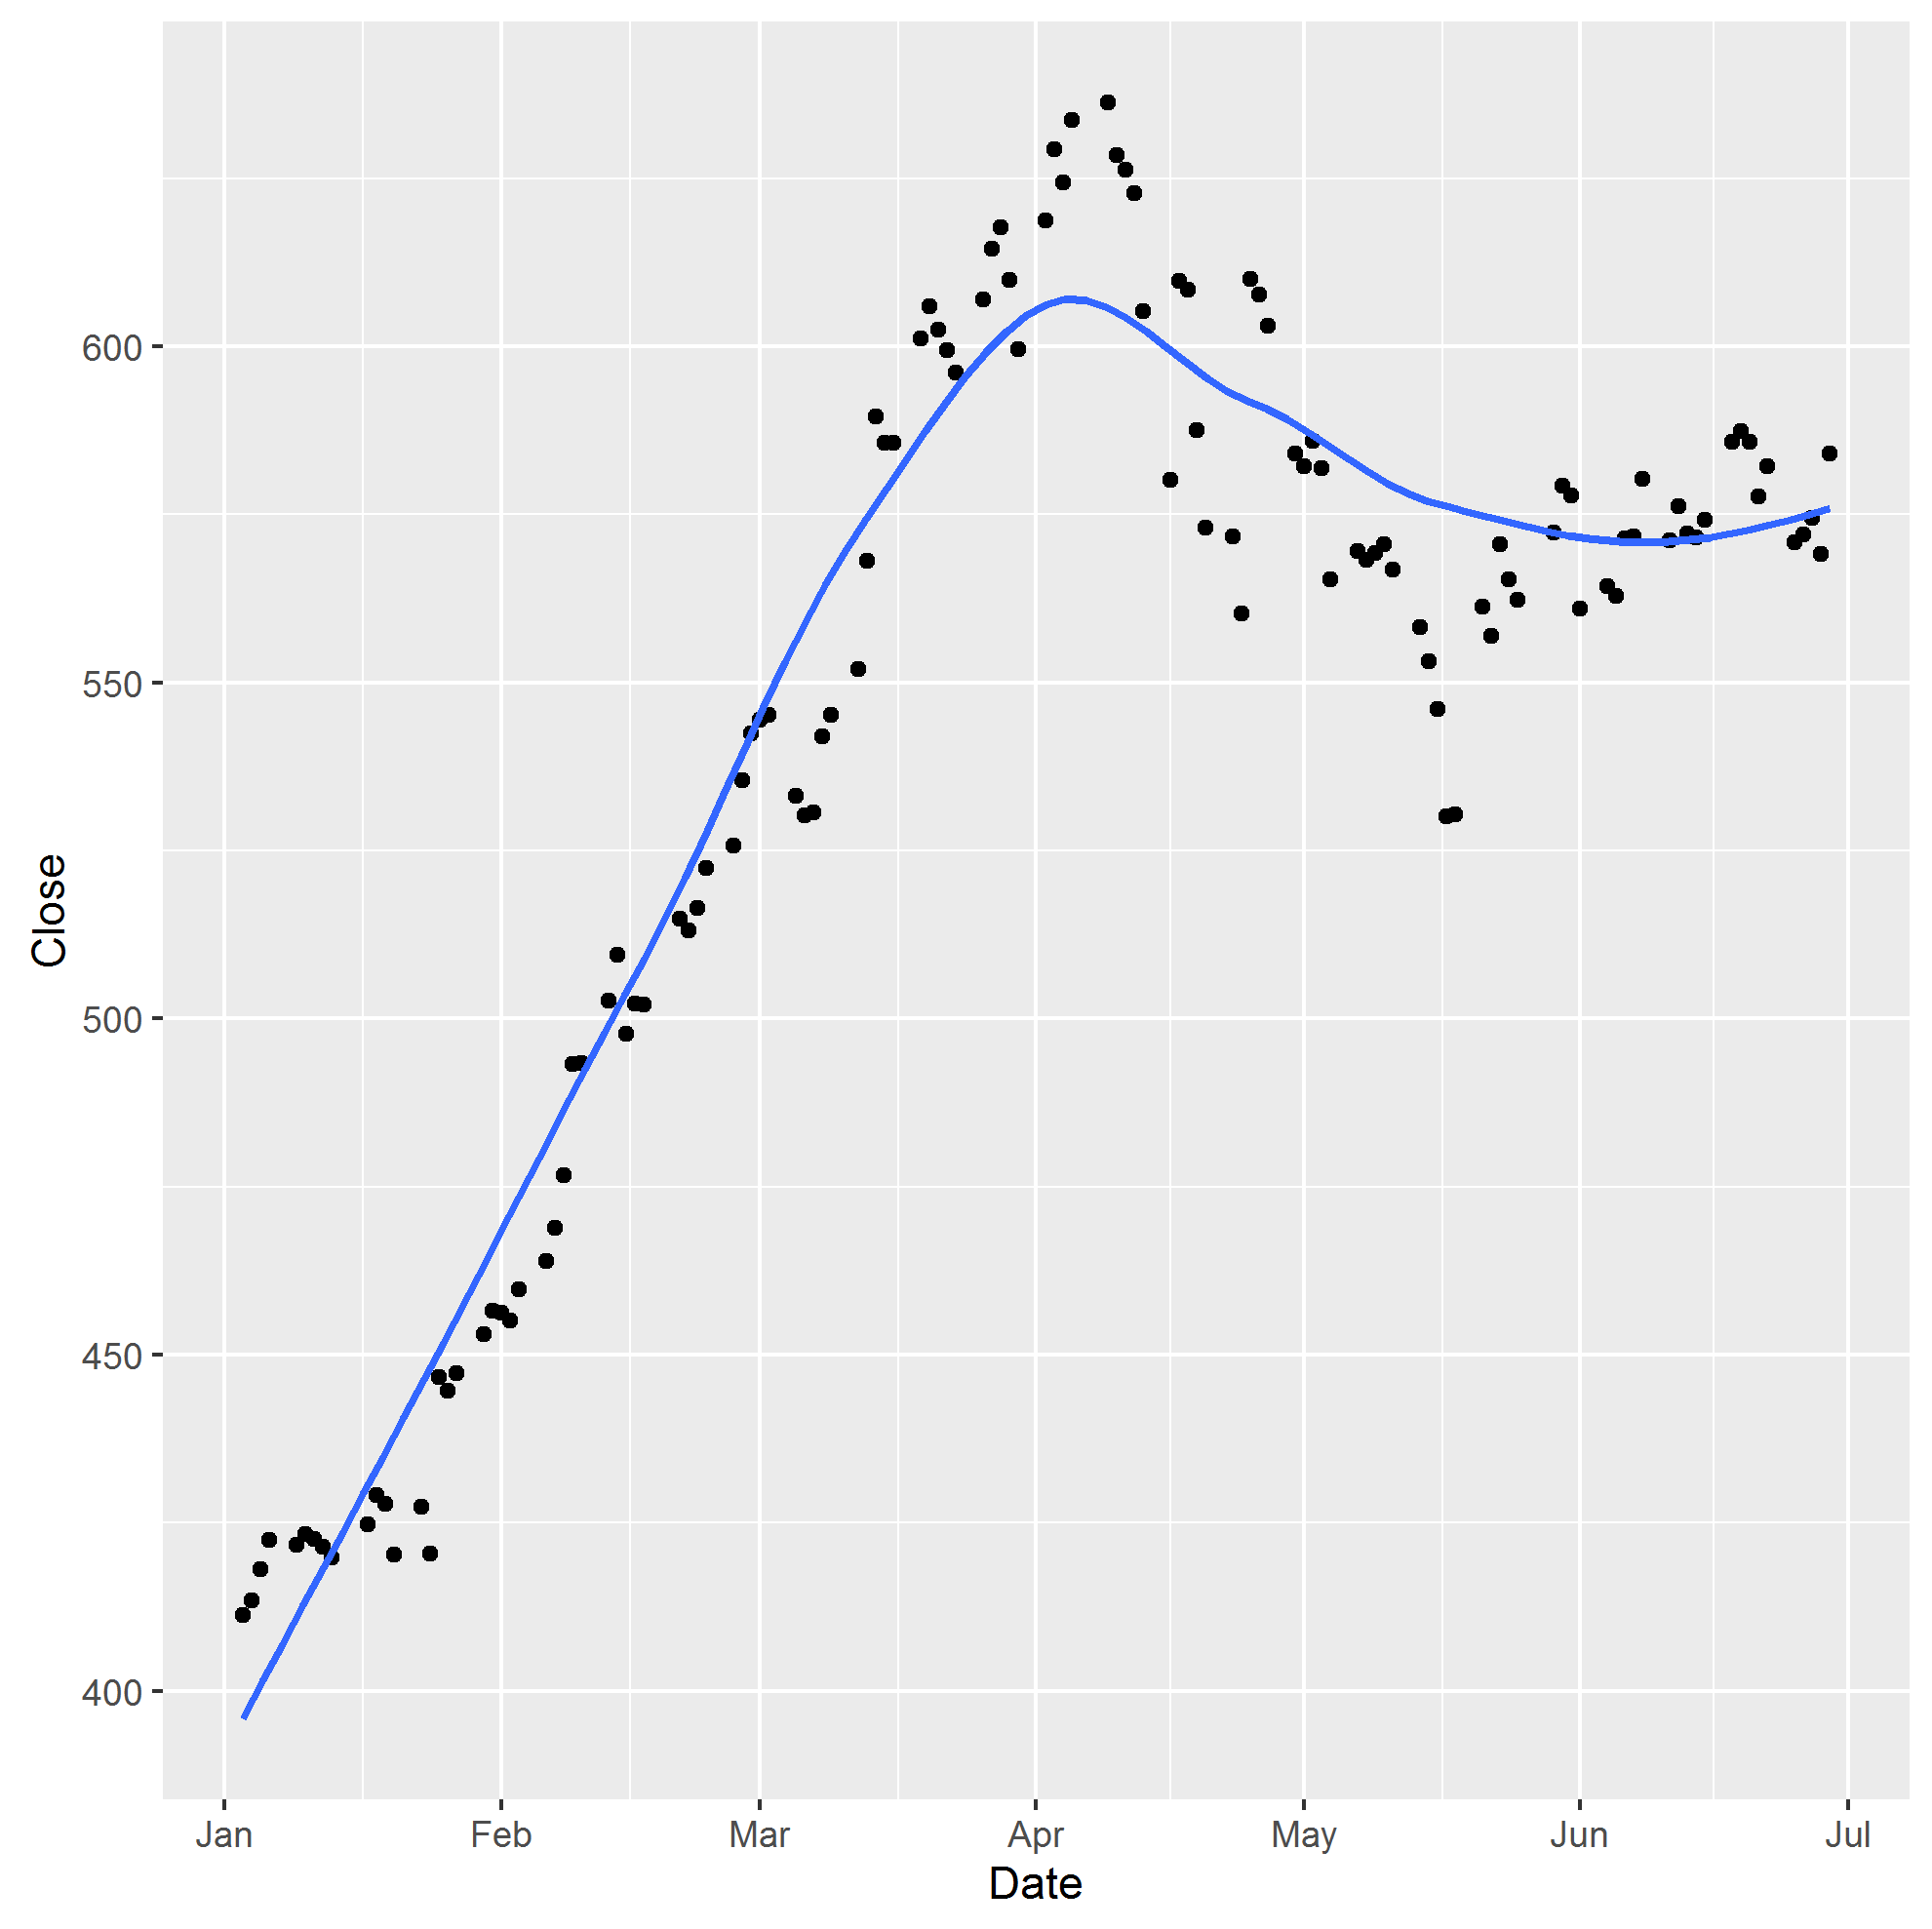
\includegraphics[width=\linewidth]{graph/AAPL3.png}
  \caption{Scatter plot with graph of Apple stock}
\endminipage\hfill
\minipage{0.46\textwidth}
  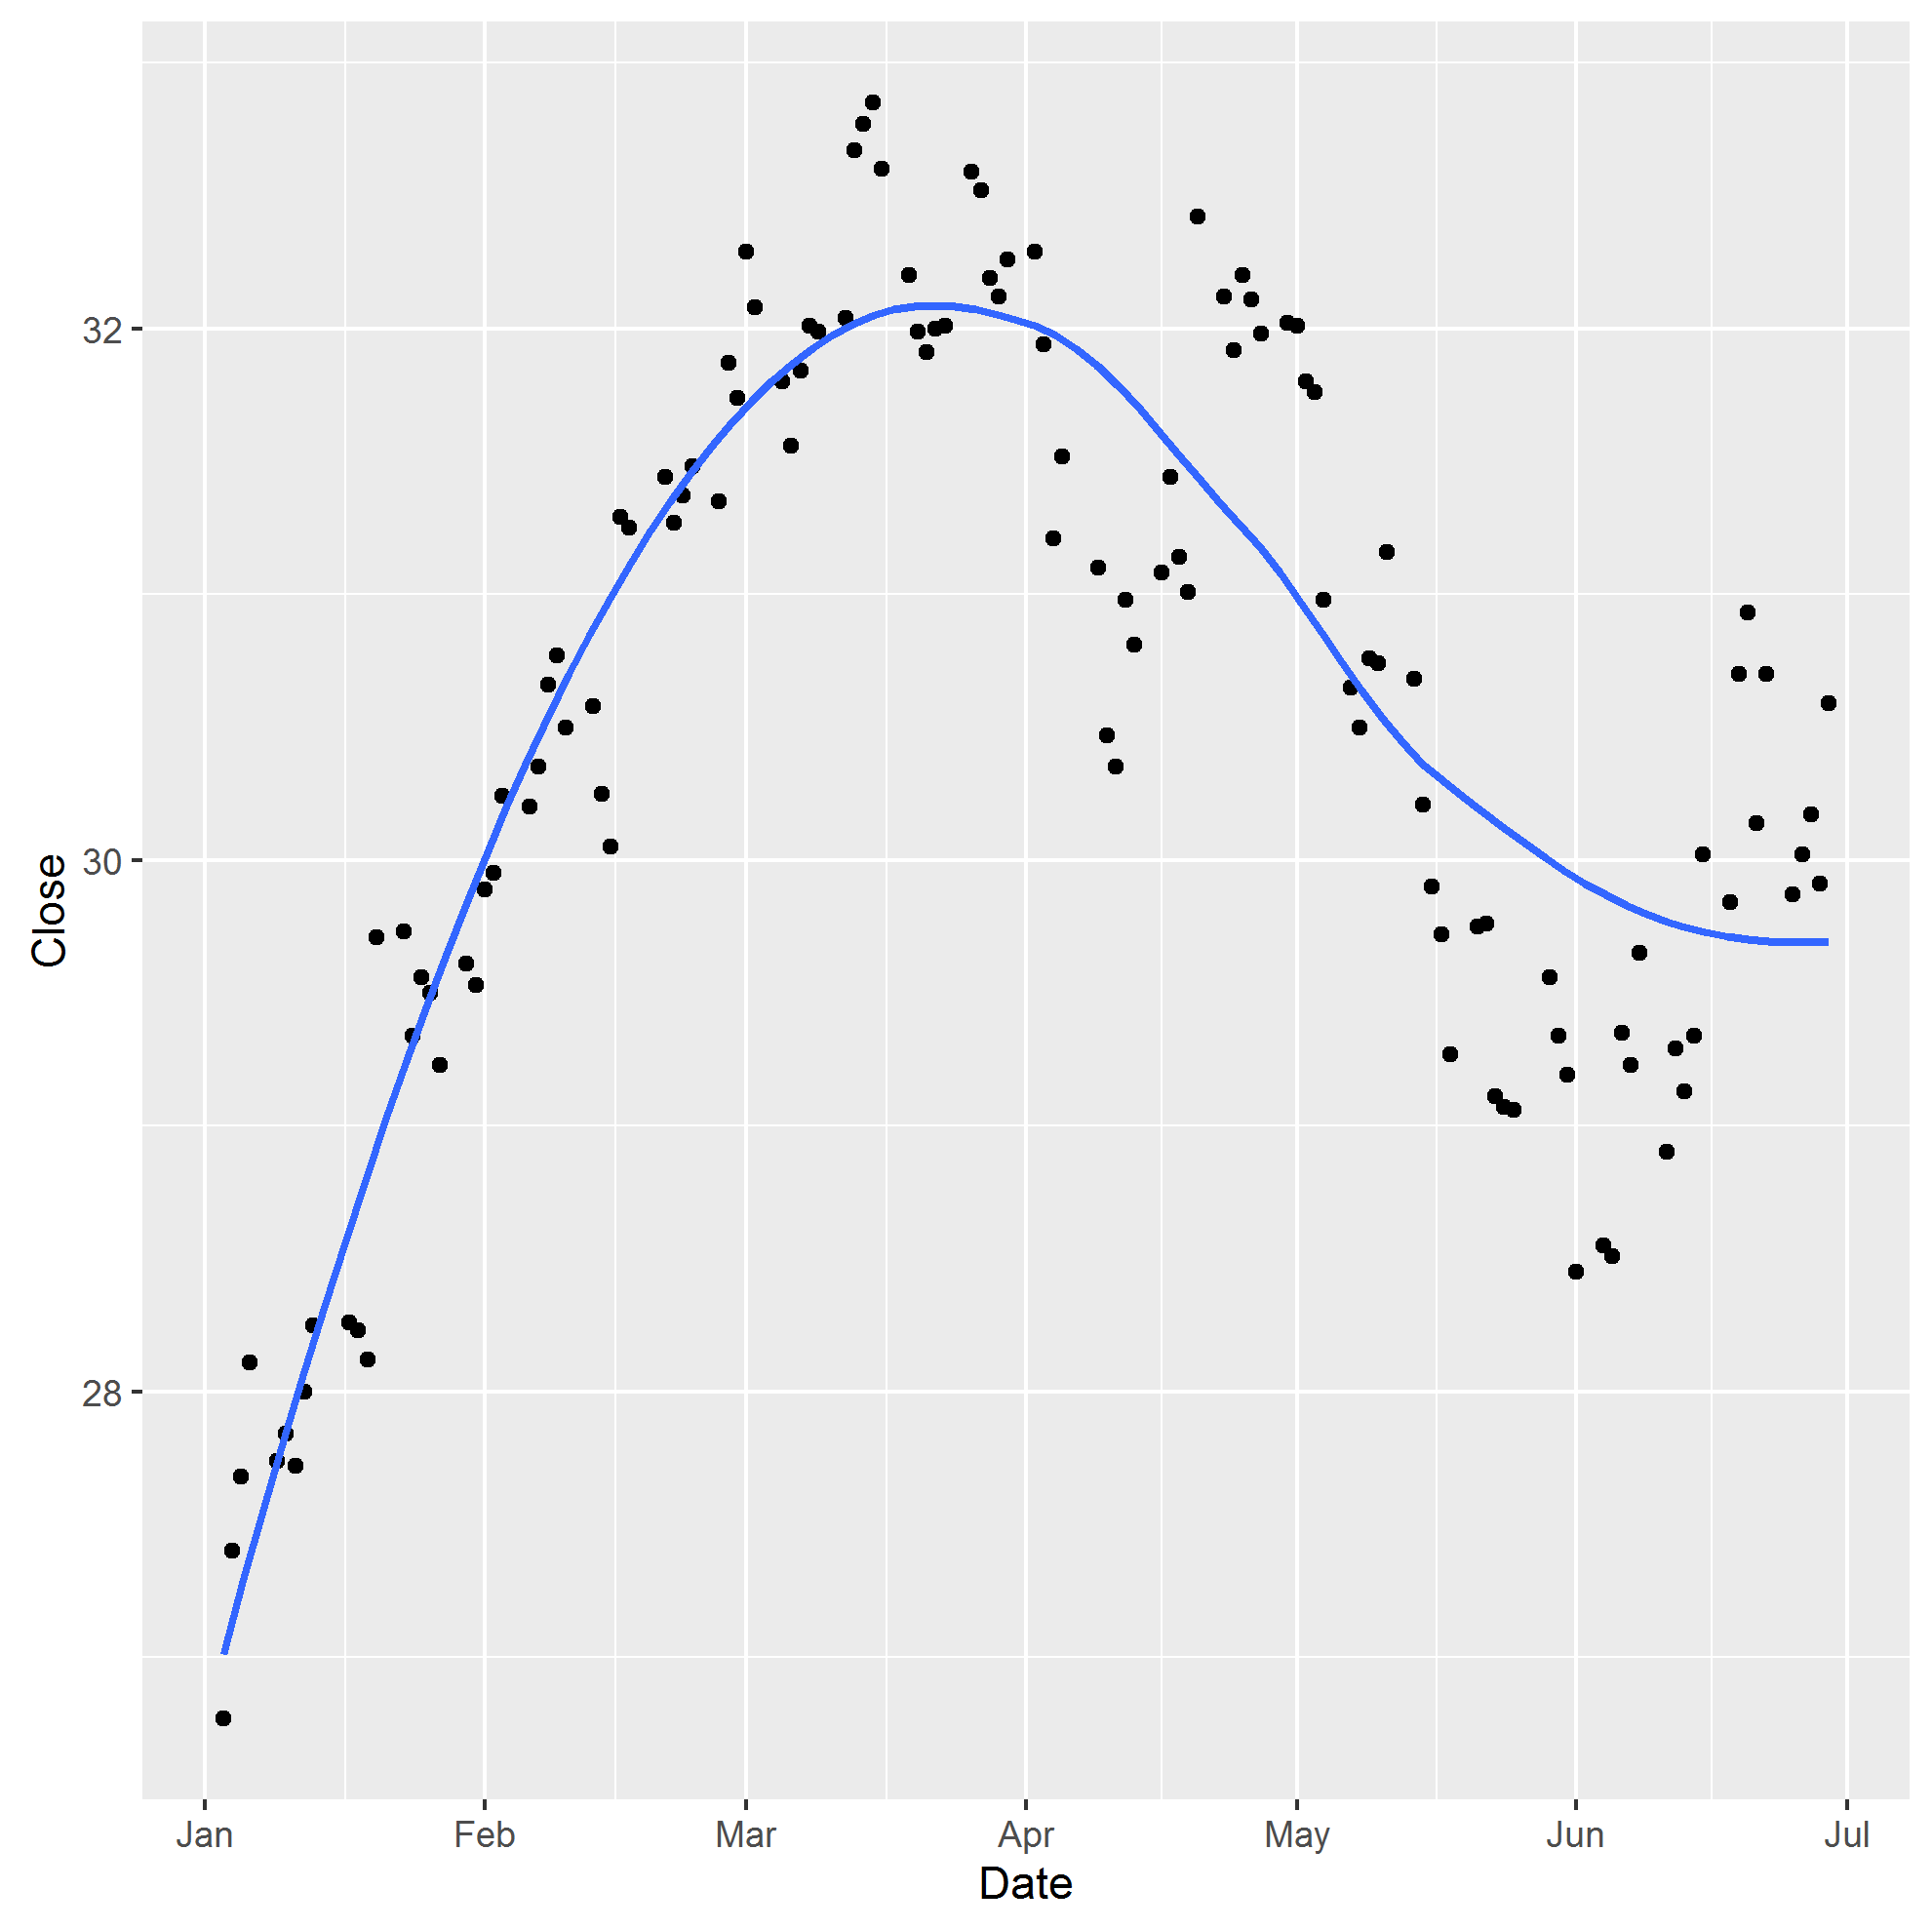
\includegraphics[width=\linewidth]{graph/MSFT3.png}
  \caption{Scatter plot with graph of Microsoft stock}
\endminipage\hfill

\end{figure}
Discuss apple chart
Discuss Microsoft chart
\subsubsection{Correlation}

\begin{figure}[!htb]
\minipage{0.8\textwidth}
  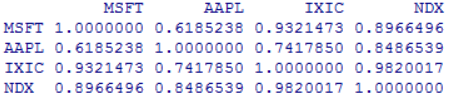
\includegraphics[width=\linewidth]{graph/cor3.png}
  \caption{Correlation table for Microsoft and Apple against two index stocks}
\endminipage\hfill
\end{figure}

Insert correlation table MS vs apple
Discuss any interesting overall observations here

\subsubsection{Regression}
Show regression lines for MS and apple. 


\begin{figure}[!htb]
\minipage{0.46\textwidth}
  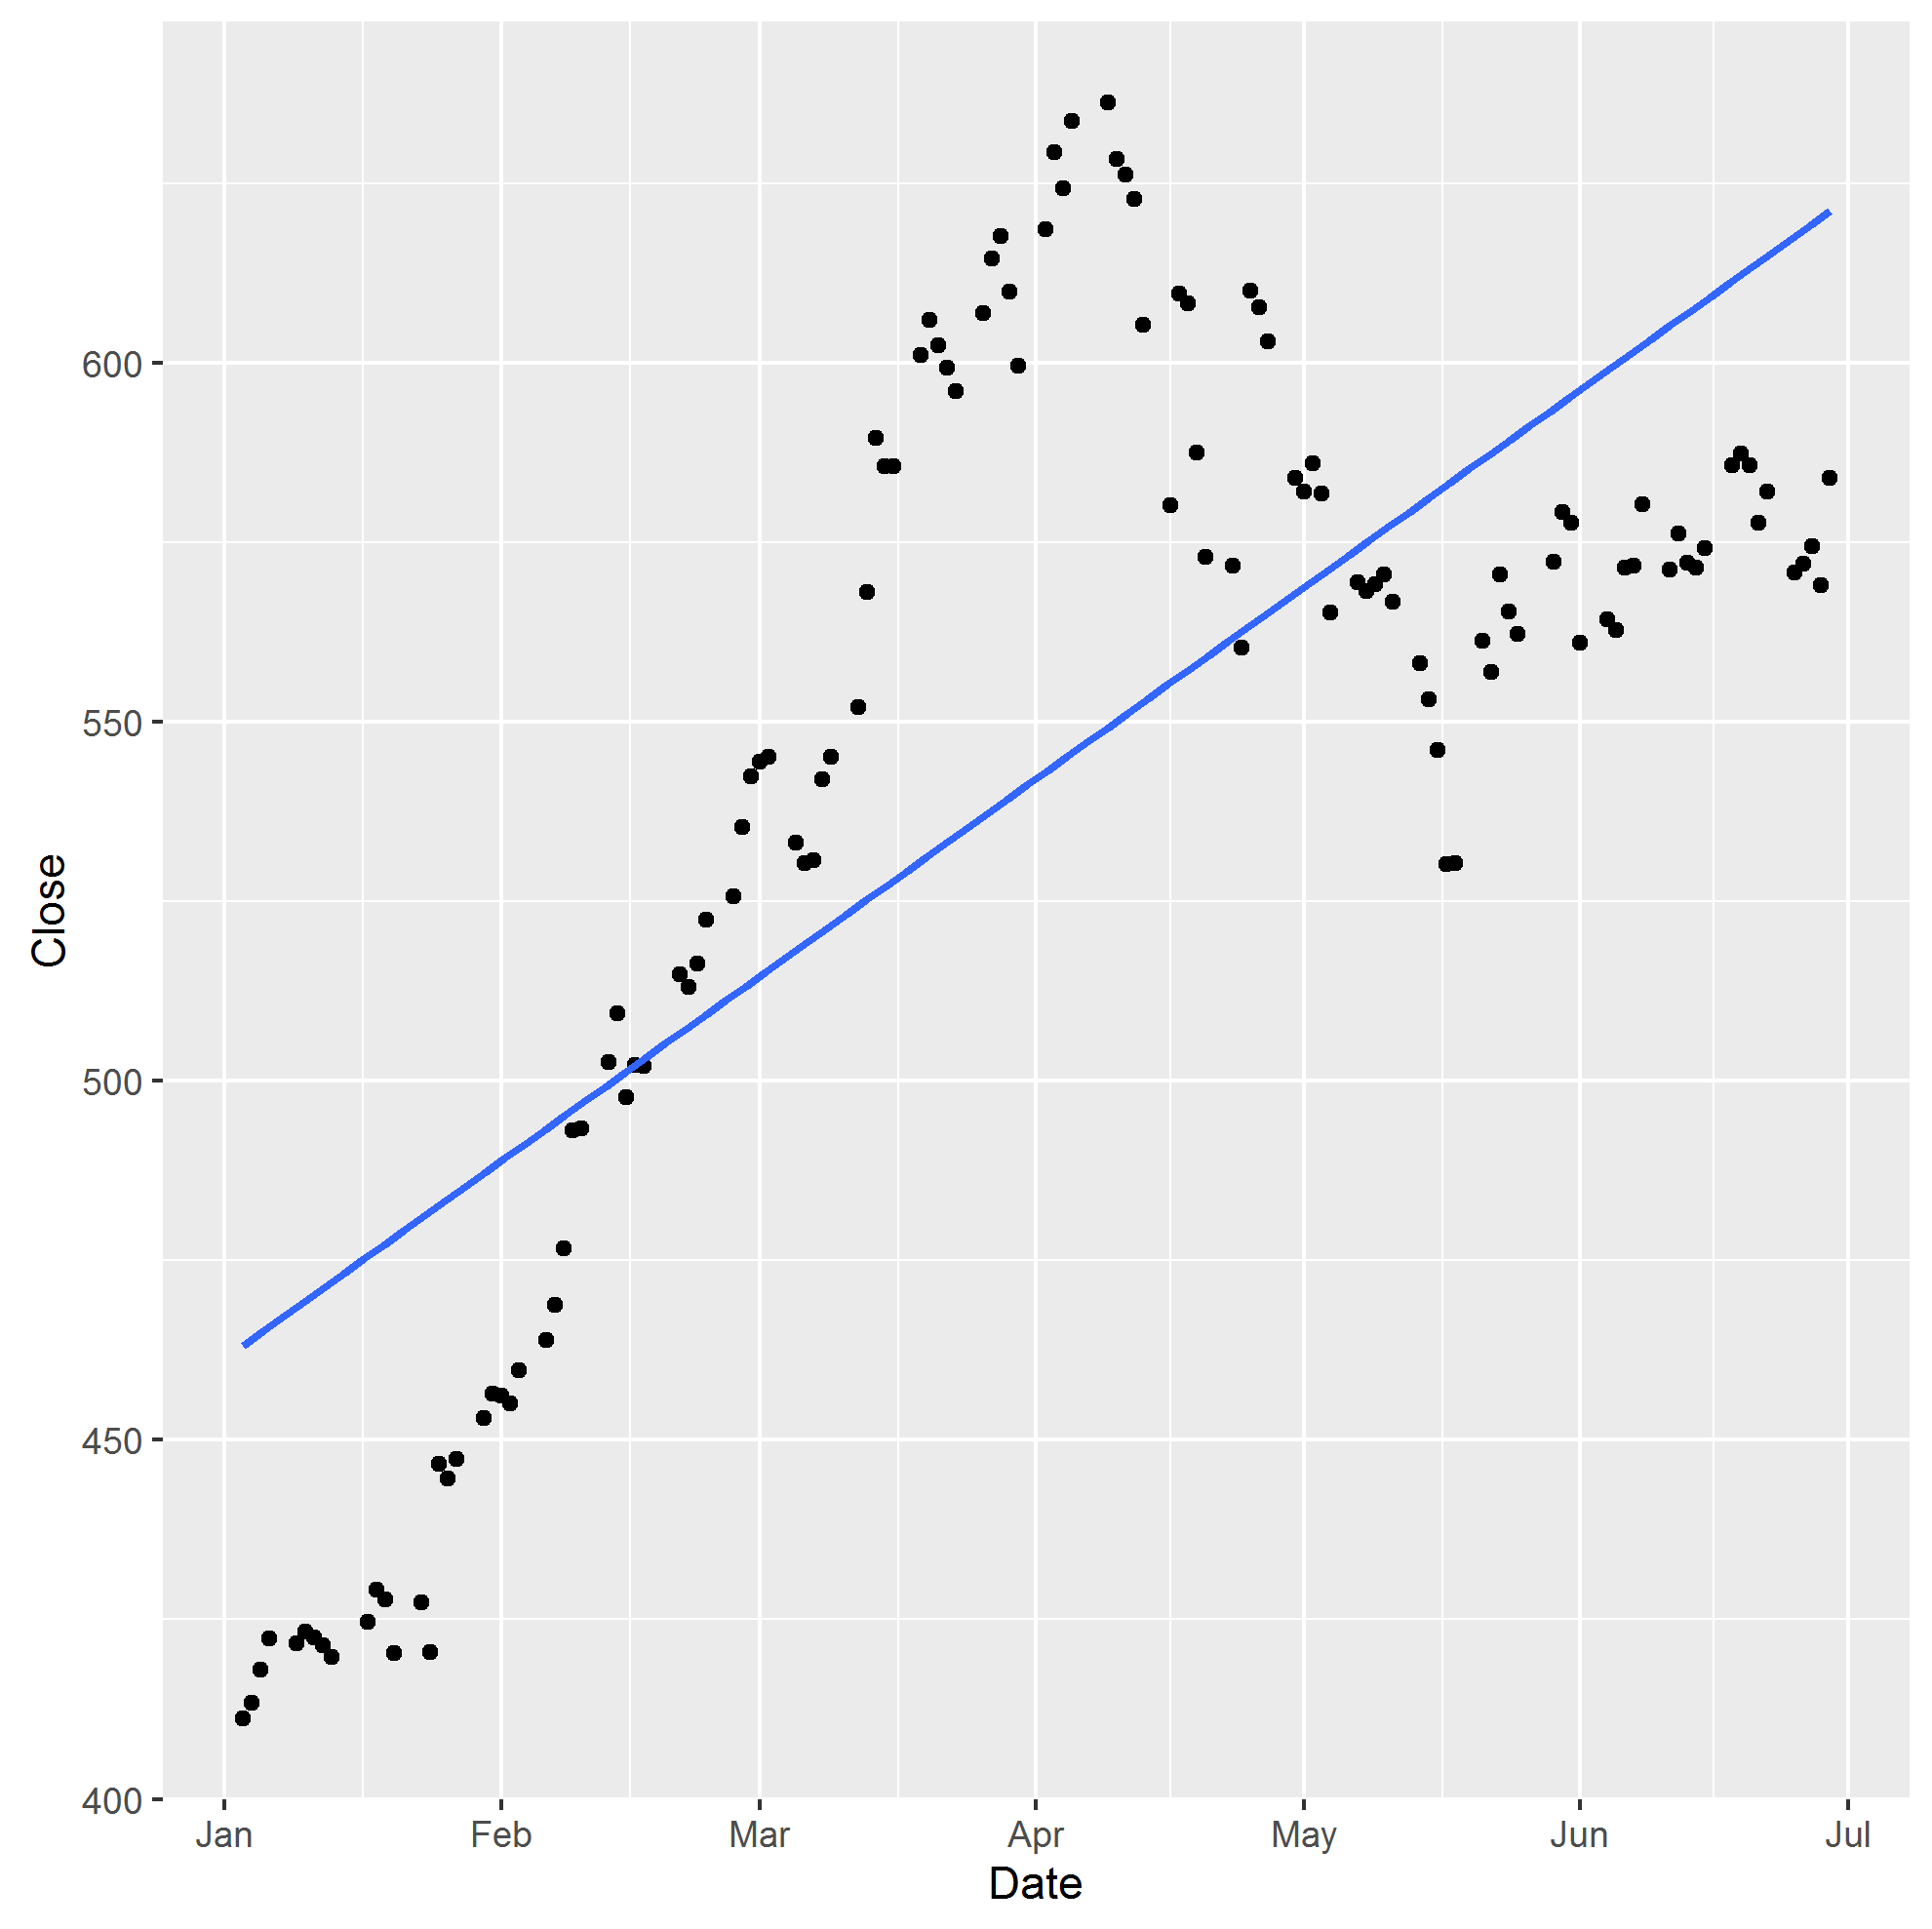
\includegraphics[width=\linewidth]{graph/a_reg3.png}
  \caption{Linear regression line of Apple closing prices.}
\endminipage\hfill
\minipage{0.46\textwidth}
  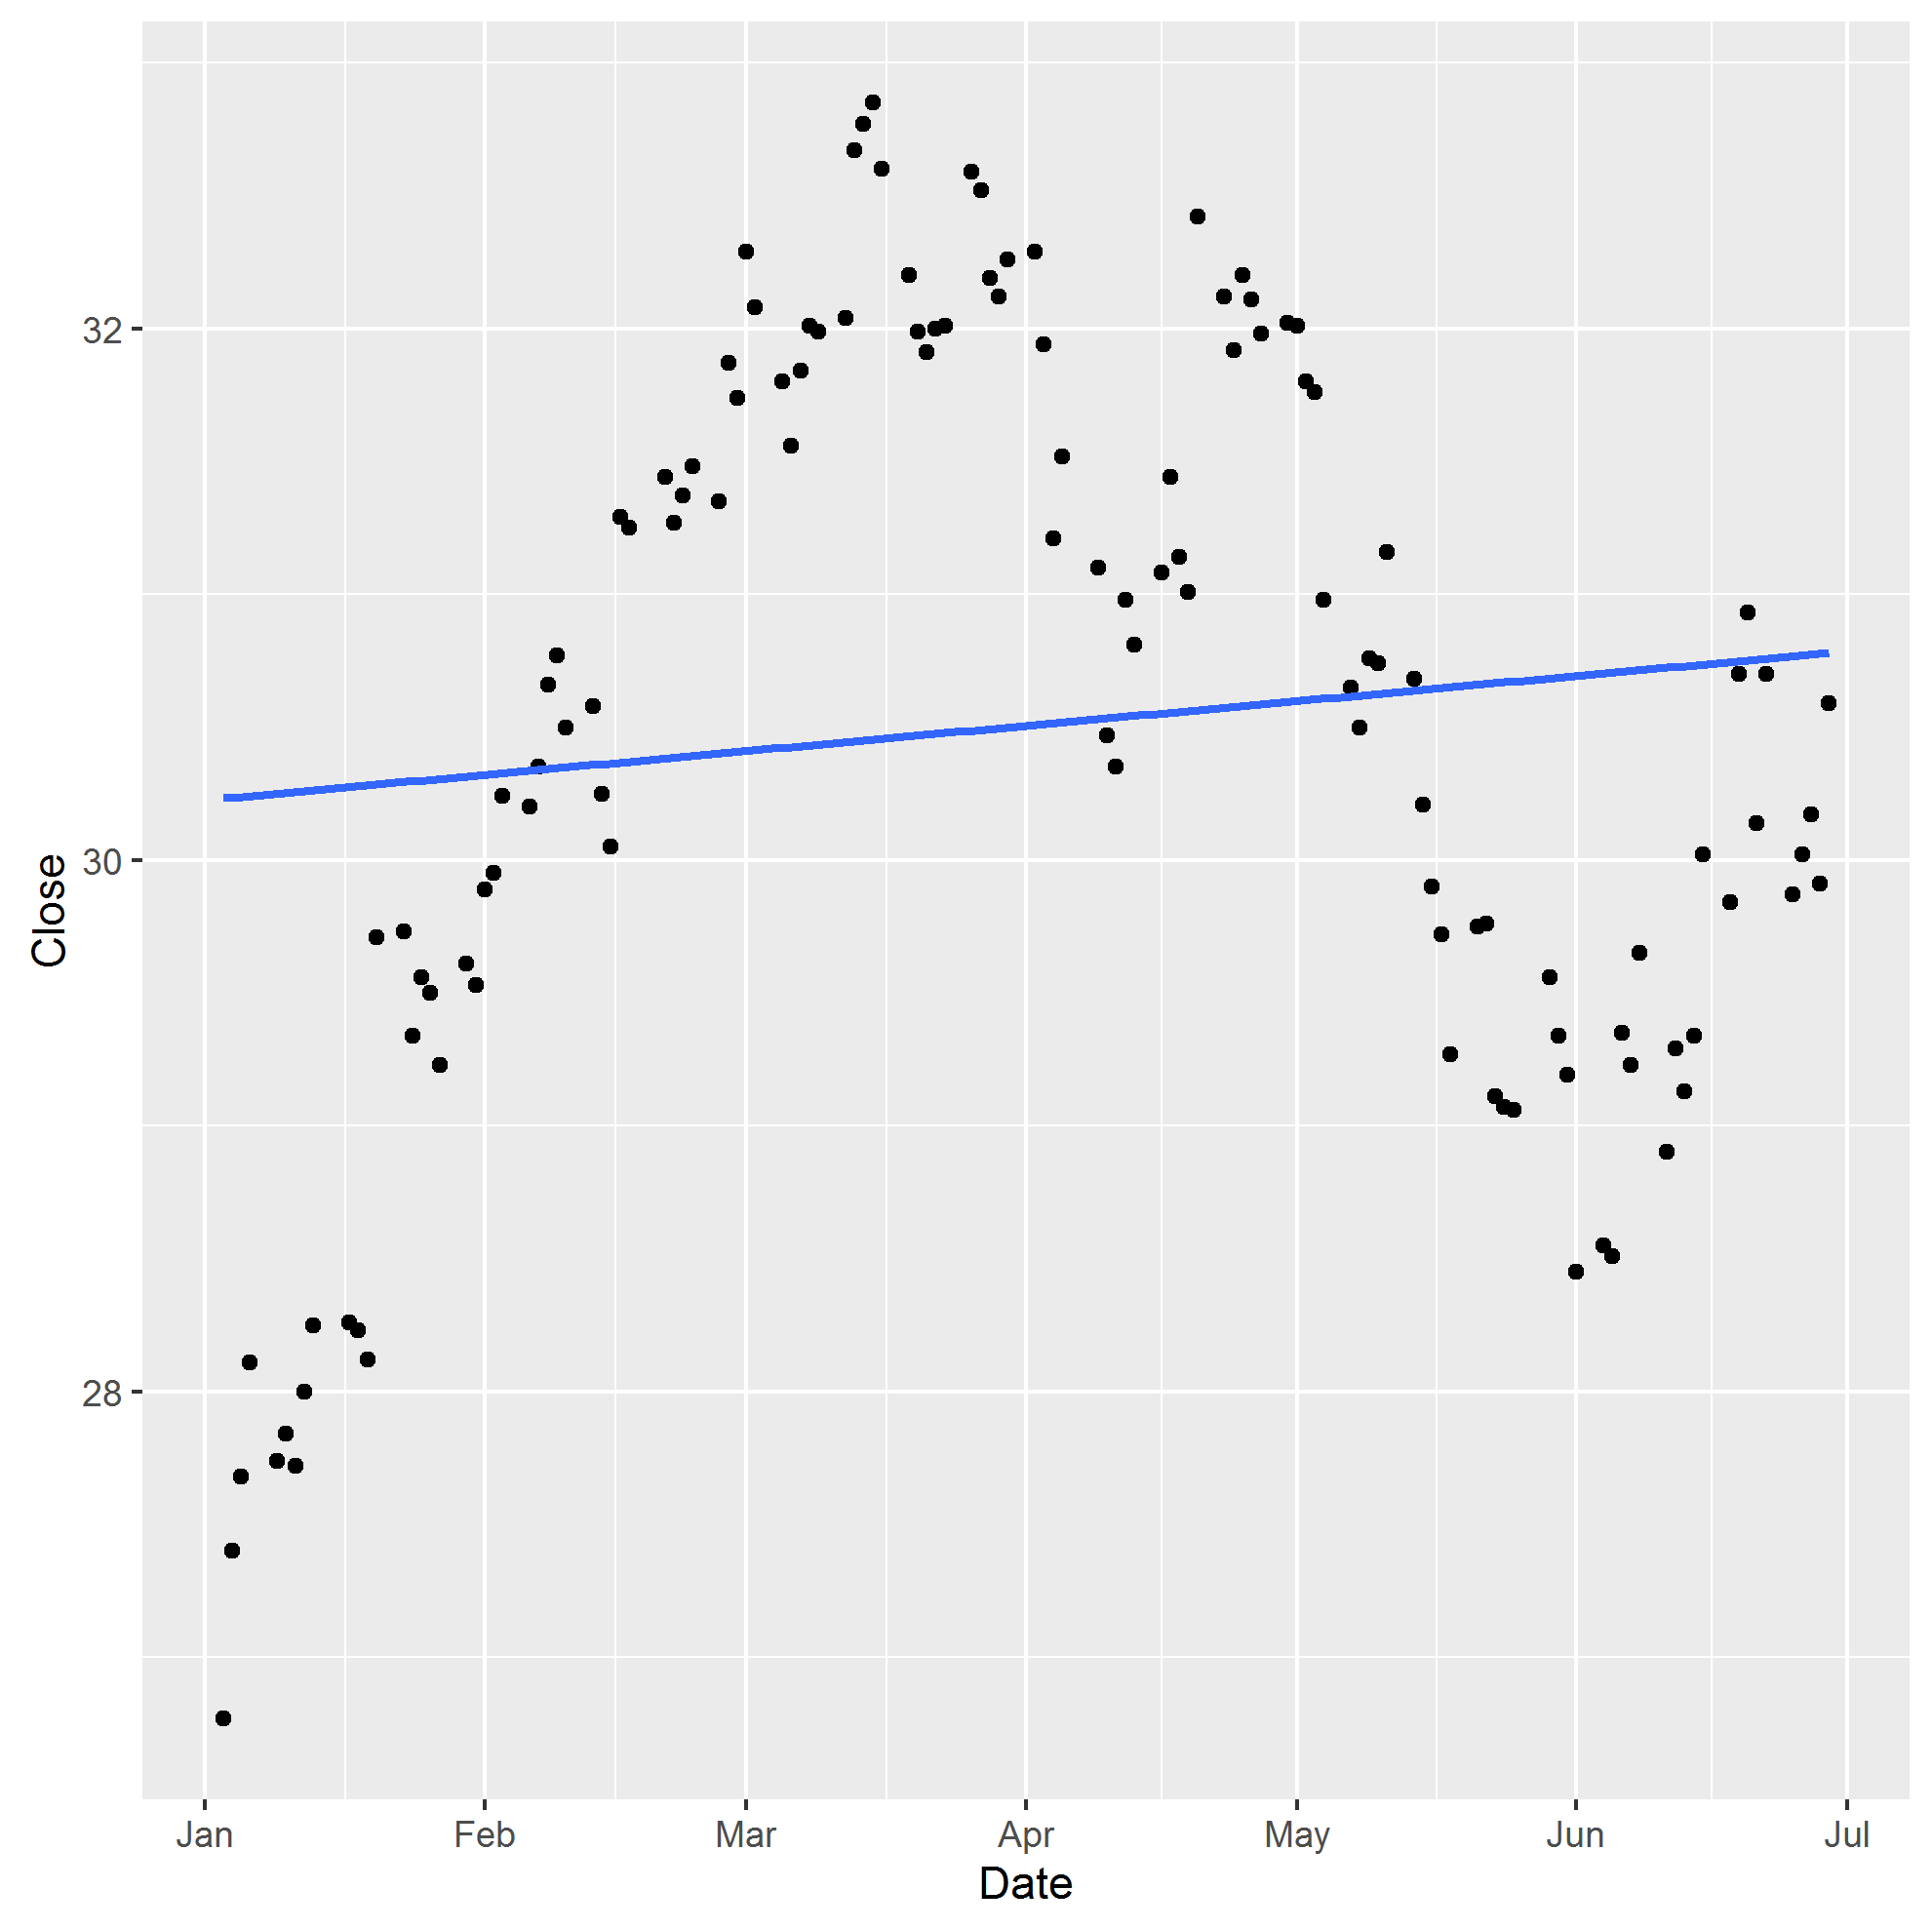
\includegraphics[width=\linewidth]{graph/m_reg3.png}
  \caption{Linear regression line of Microsoft closing prices.}
\endminipage\hfill
\end{figure}

Discuss regression lines. 

List y intercept, slope overall. 

\begin{figure}[!htb]
\minipage{0.46\textwidth}
  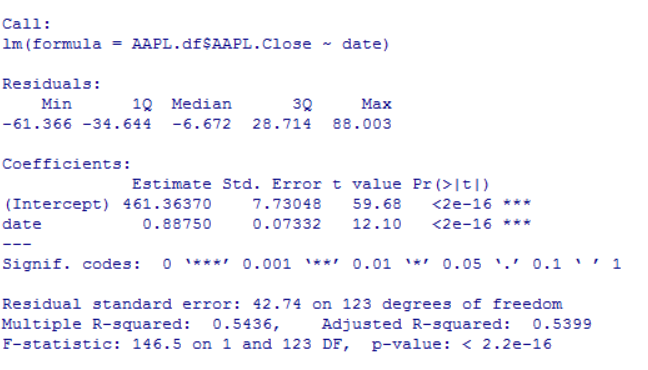
\includegraphics[width=\linewidth]{graph/aapl_reg_3.png}
  \caption{Linear regression line of Apple closing prices.}
\endminipage\hfill
\minipage{0.46\textwidth}
  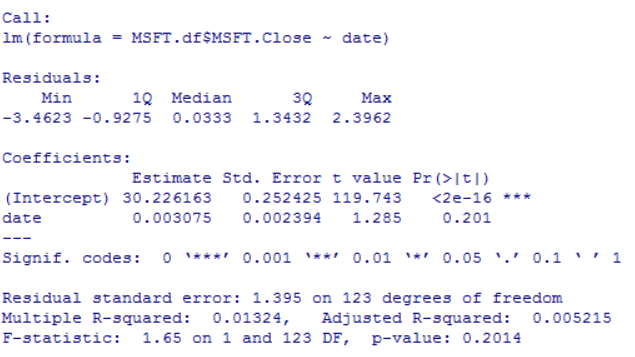
\includegraphics[width=\linewidth]{graph/msft_reg_3.png}
  \caption{Linear regression line of Microsoft closing prices.}
\endminipage\hfill
\end{figure}



\subsubsection{Analysis}
Discuss any interesting overall observations here

\subsection{July - December  2012 }
\subsubsection{Plots}
\begin{figure}[!htb]
\minipage{0.46\textwidth}
  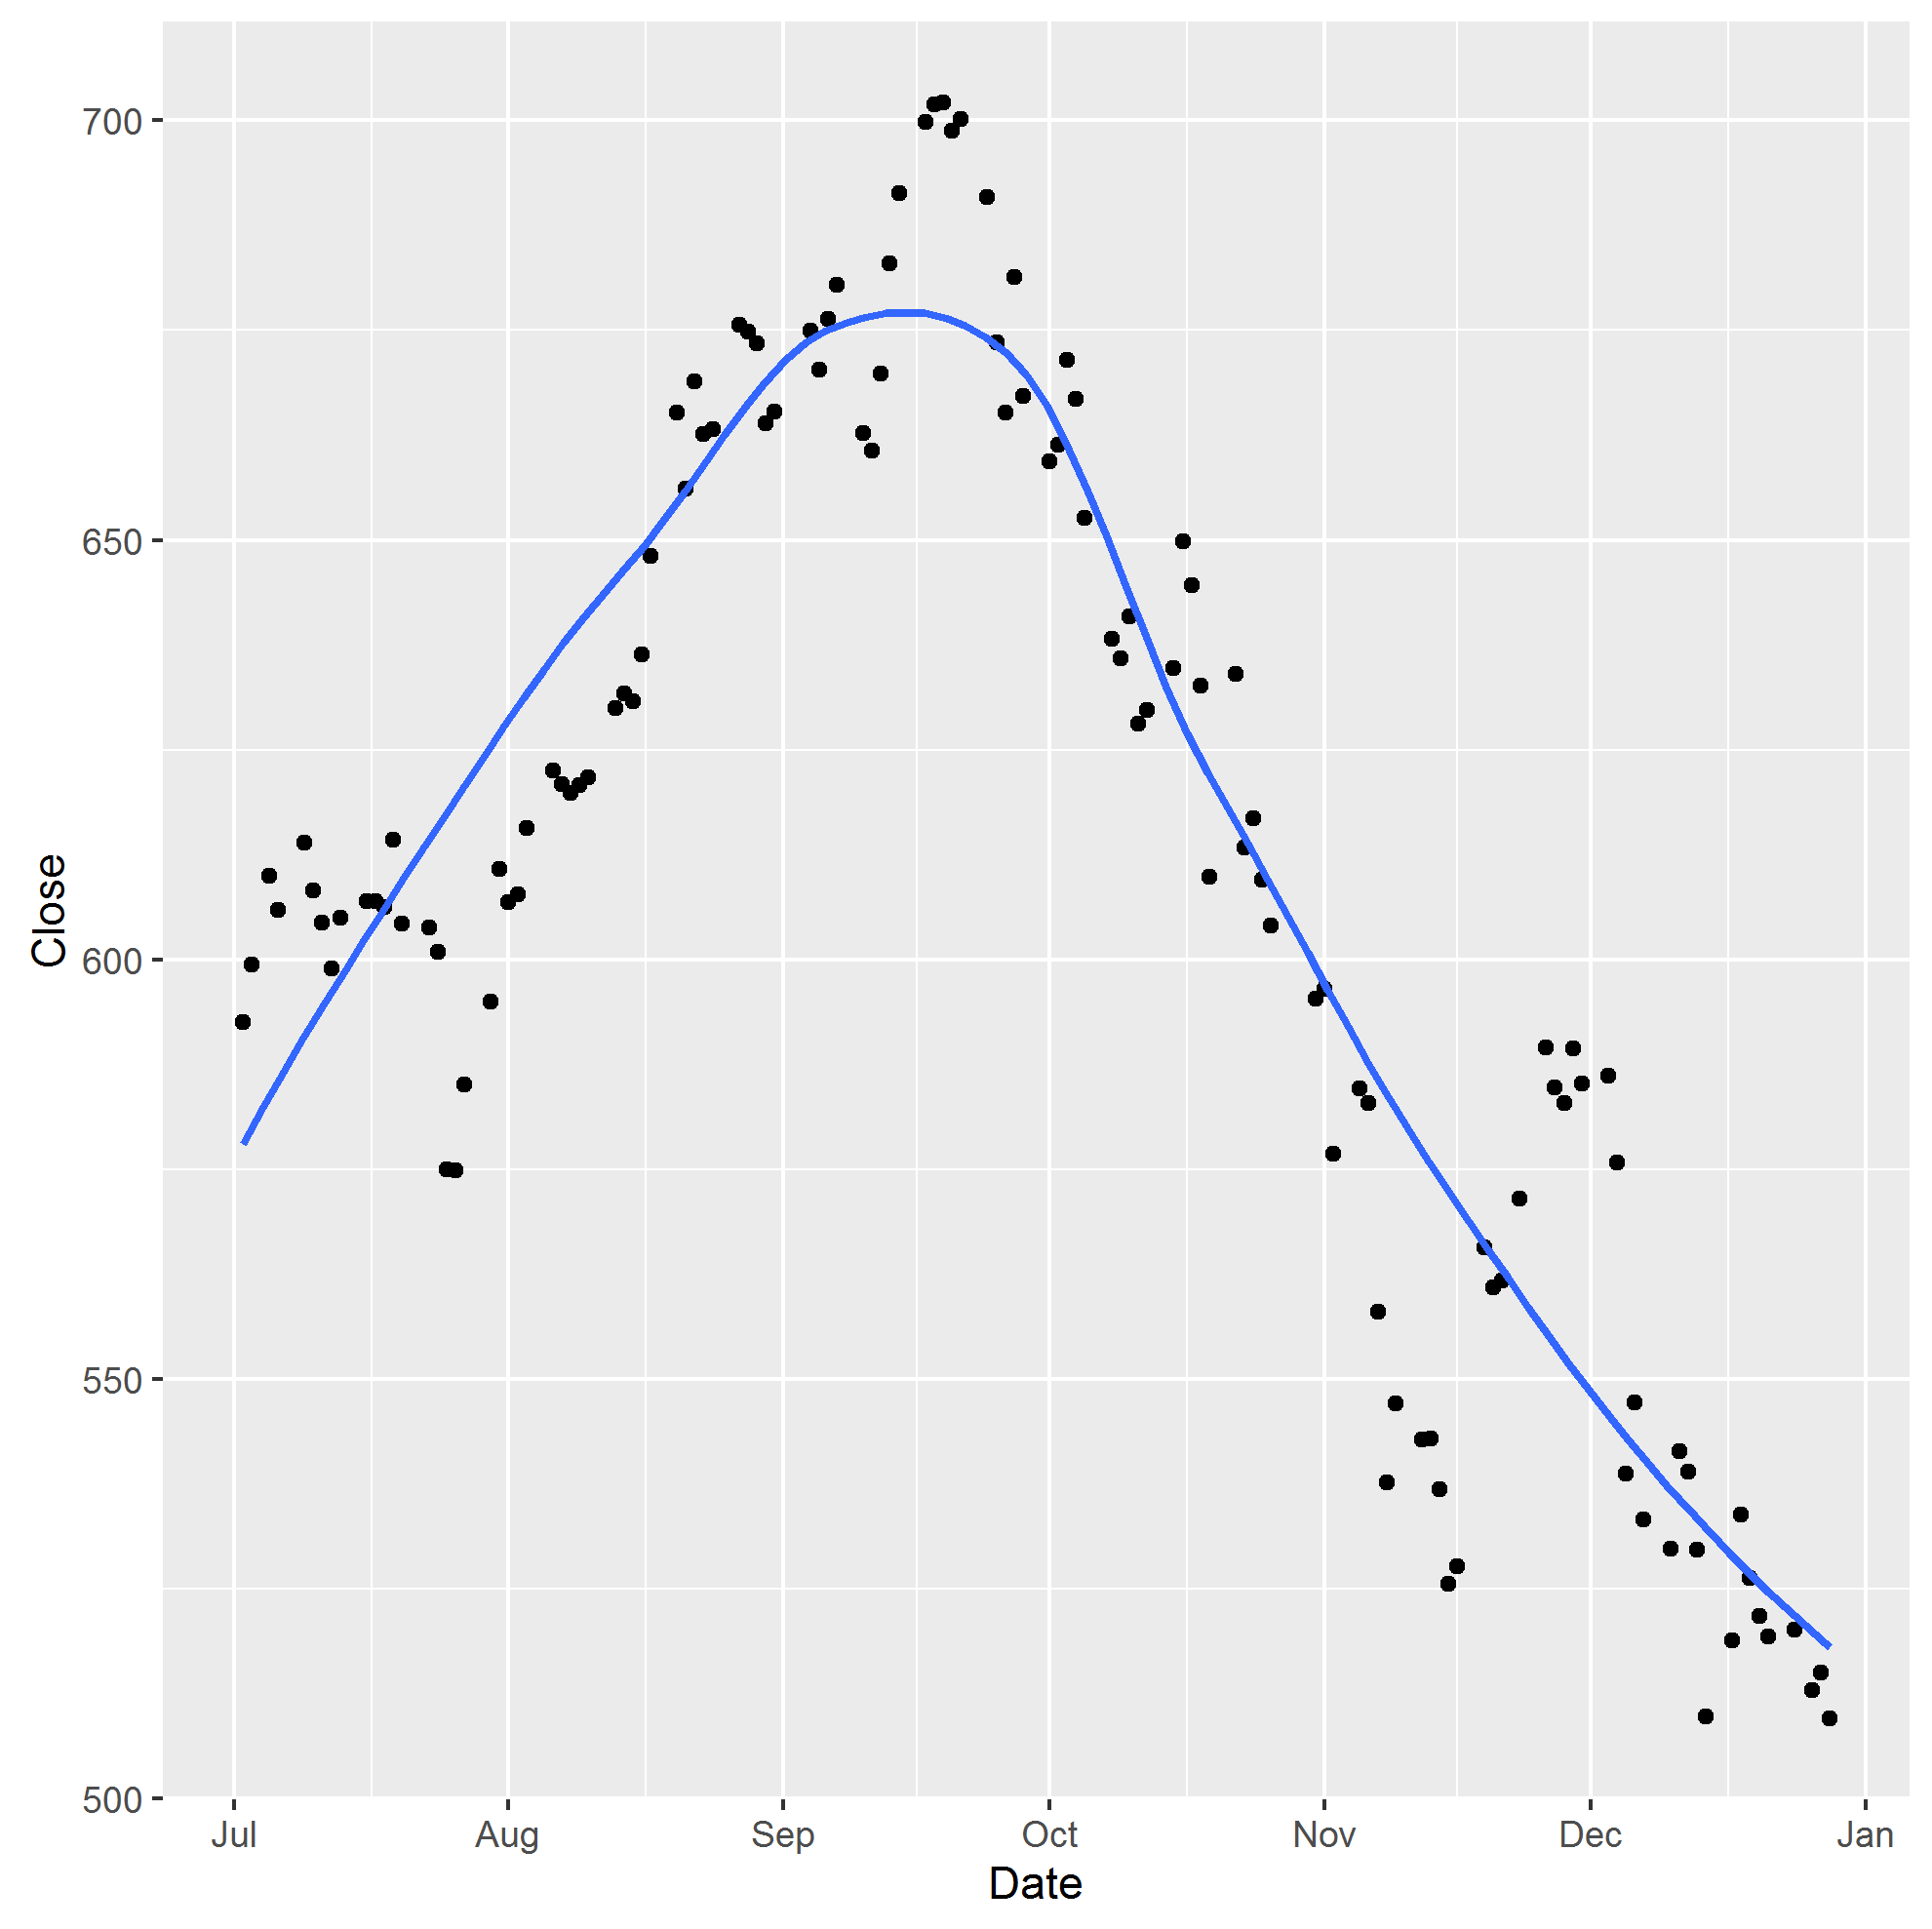
\includegraphics[width=\linewidth]{graph/AAPL4.png}
  \caption{Scatter plot with graph of Apple stock}
\endminipage\hfill
\minipage{0.46\textwidth}
  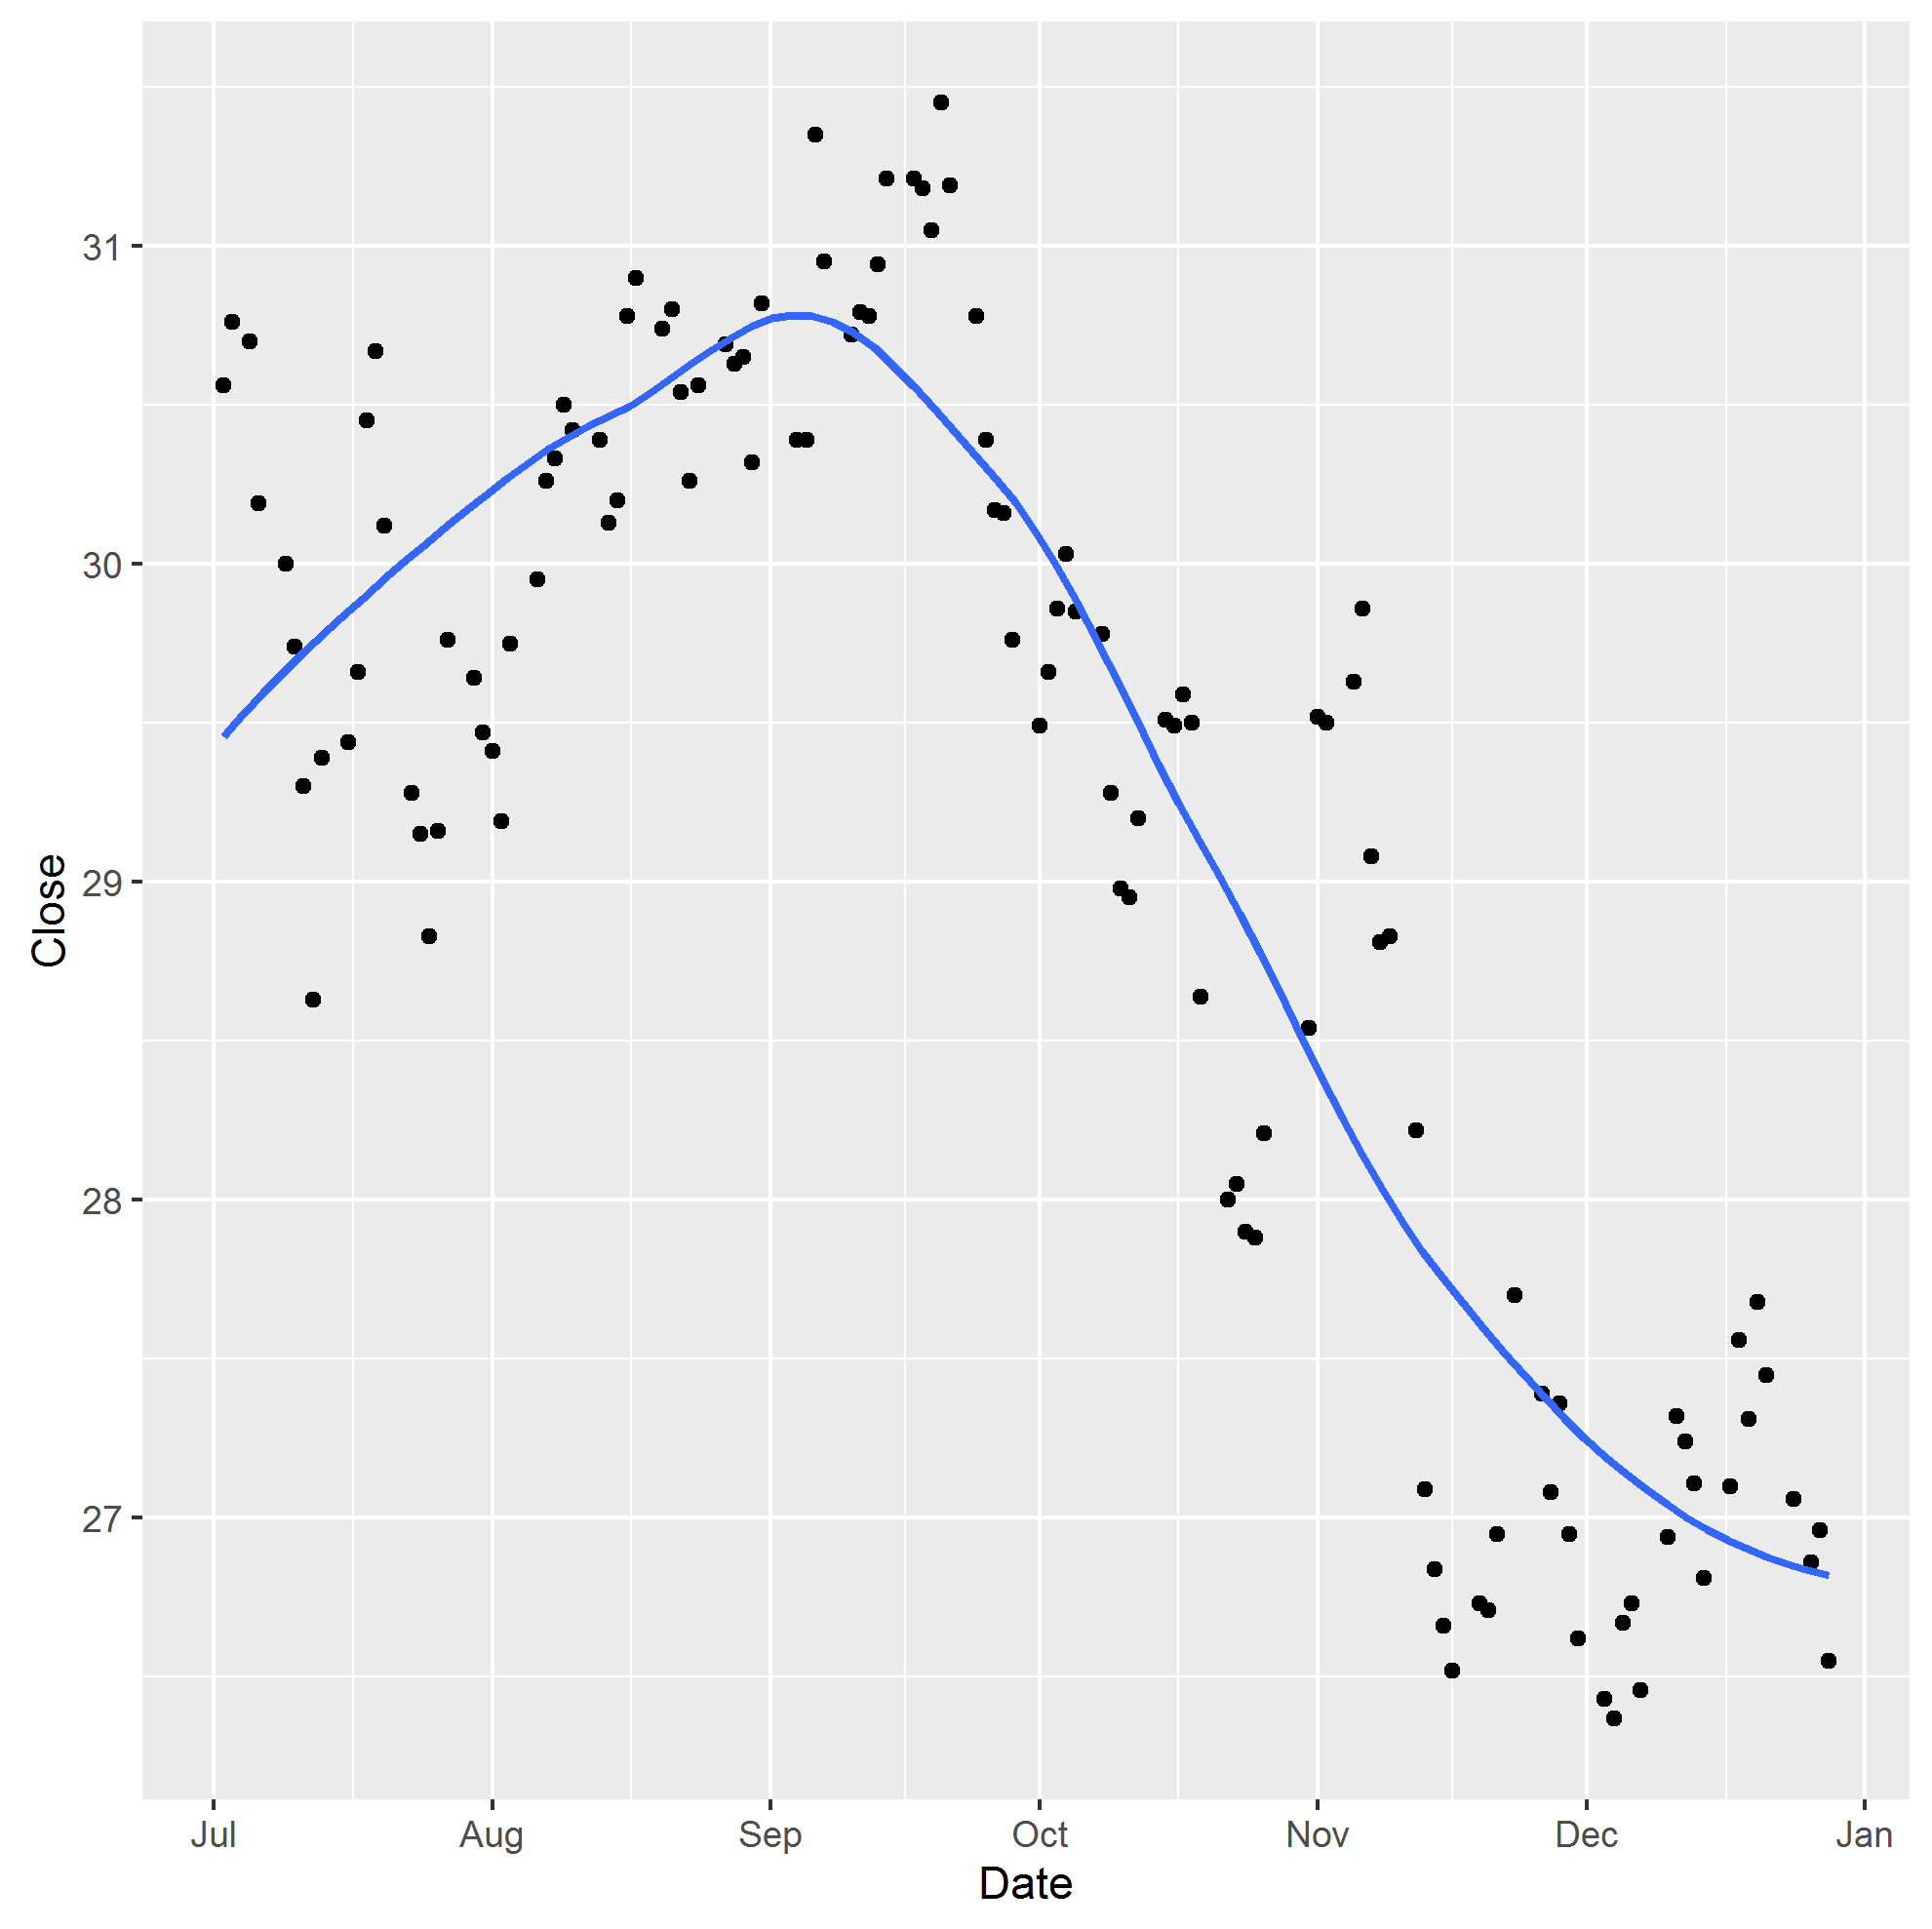
\includegraphics[width=\linewidth]{graph/MSFT4.png}
  \caption{Scatter plot with graph of Microsoft stock}
\endminipage\hfill

\end{figure}
Discuss apple chart
Discuss Microsoft chart
\subsubsection{Correlation}

\begin{figure}[!htb]
\minipage{0.8\textwidth}
  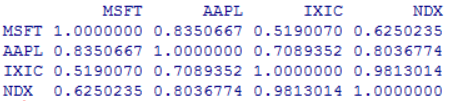
\includegraphics[width=\linewidth]{graph/cor4.png}
  \caption{Correlation table for Microsoft and Apple against two index stocks}
\endminipage\hfill
\end{figure}

Insert correlation table MS vs apple
Discuss any interesting overall observations here

\subsubsection{Regression}
Show regression lines for MS and apple. 


\begin{figure}[!htb]
\minipage{0.46\textwidth}
  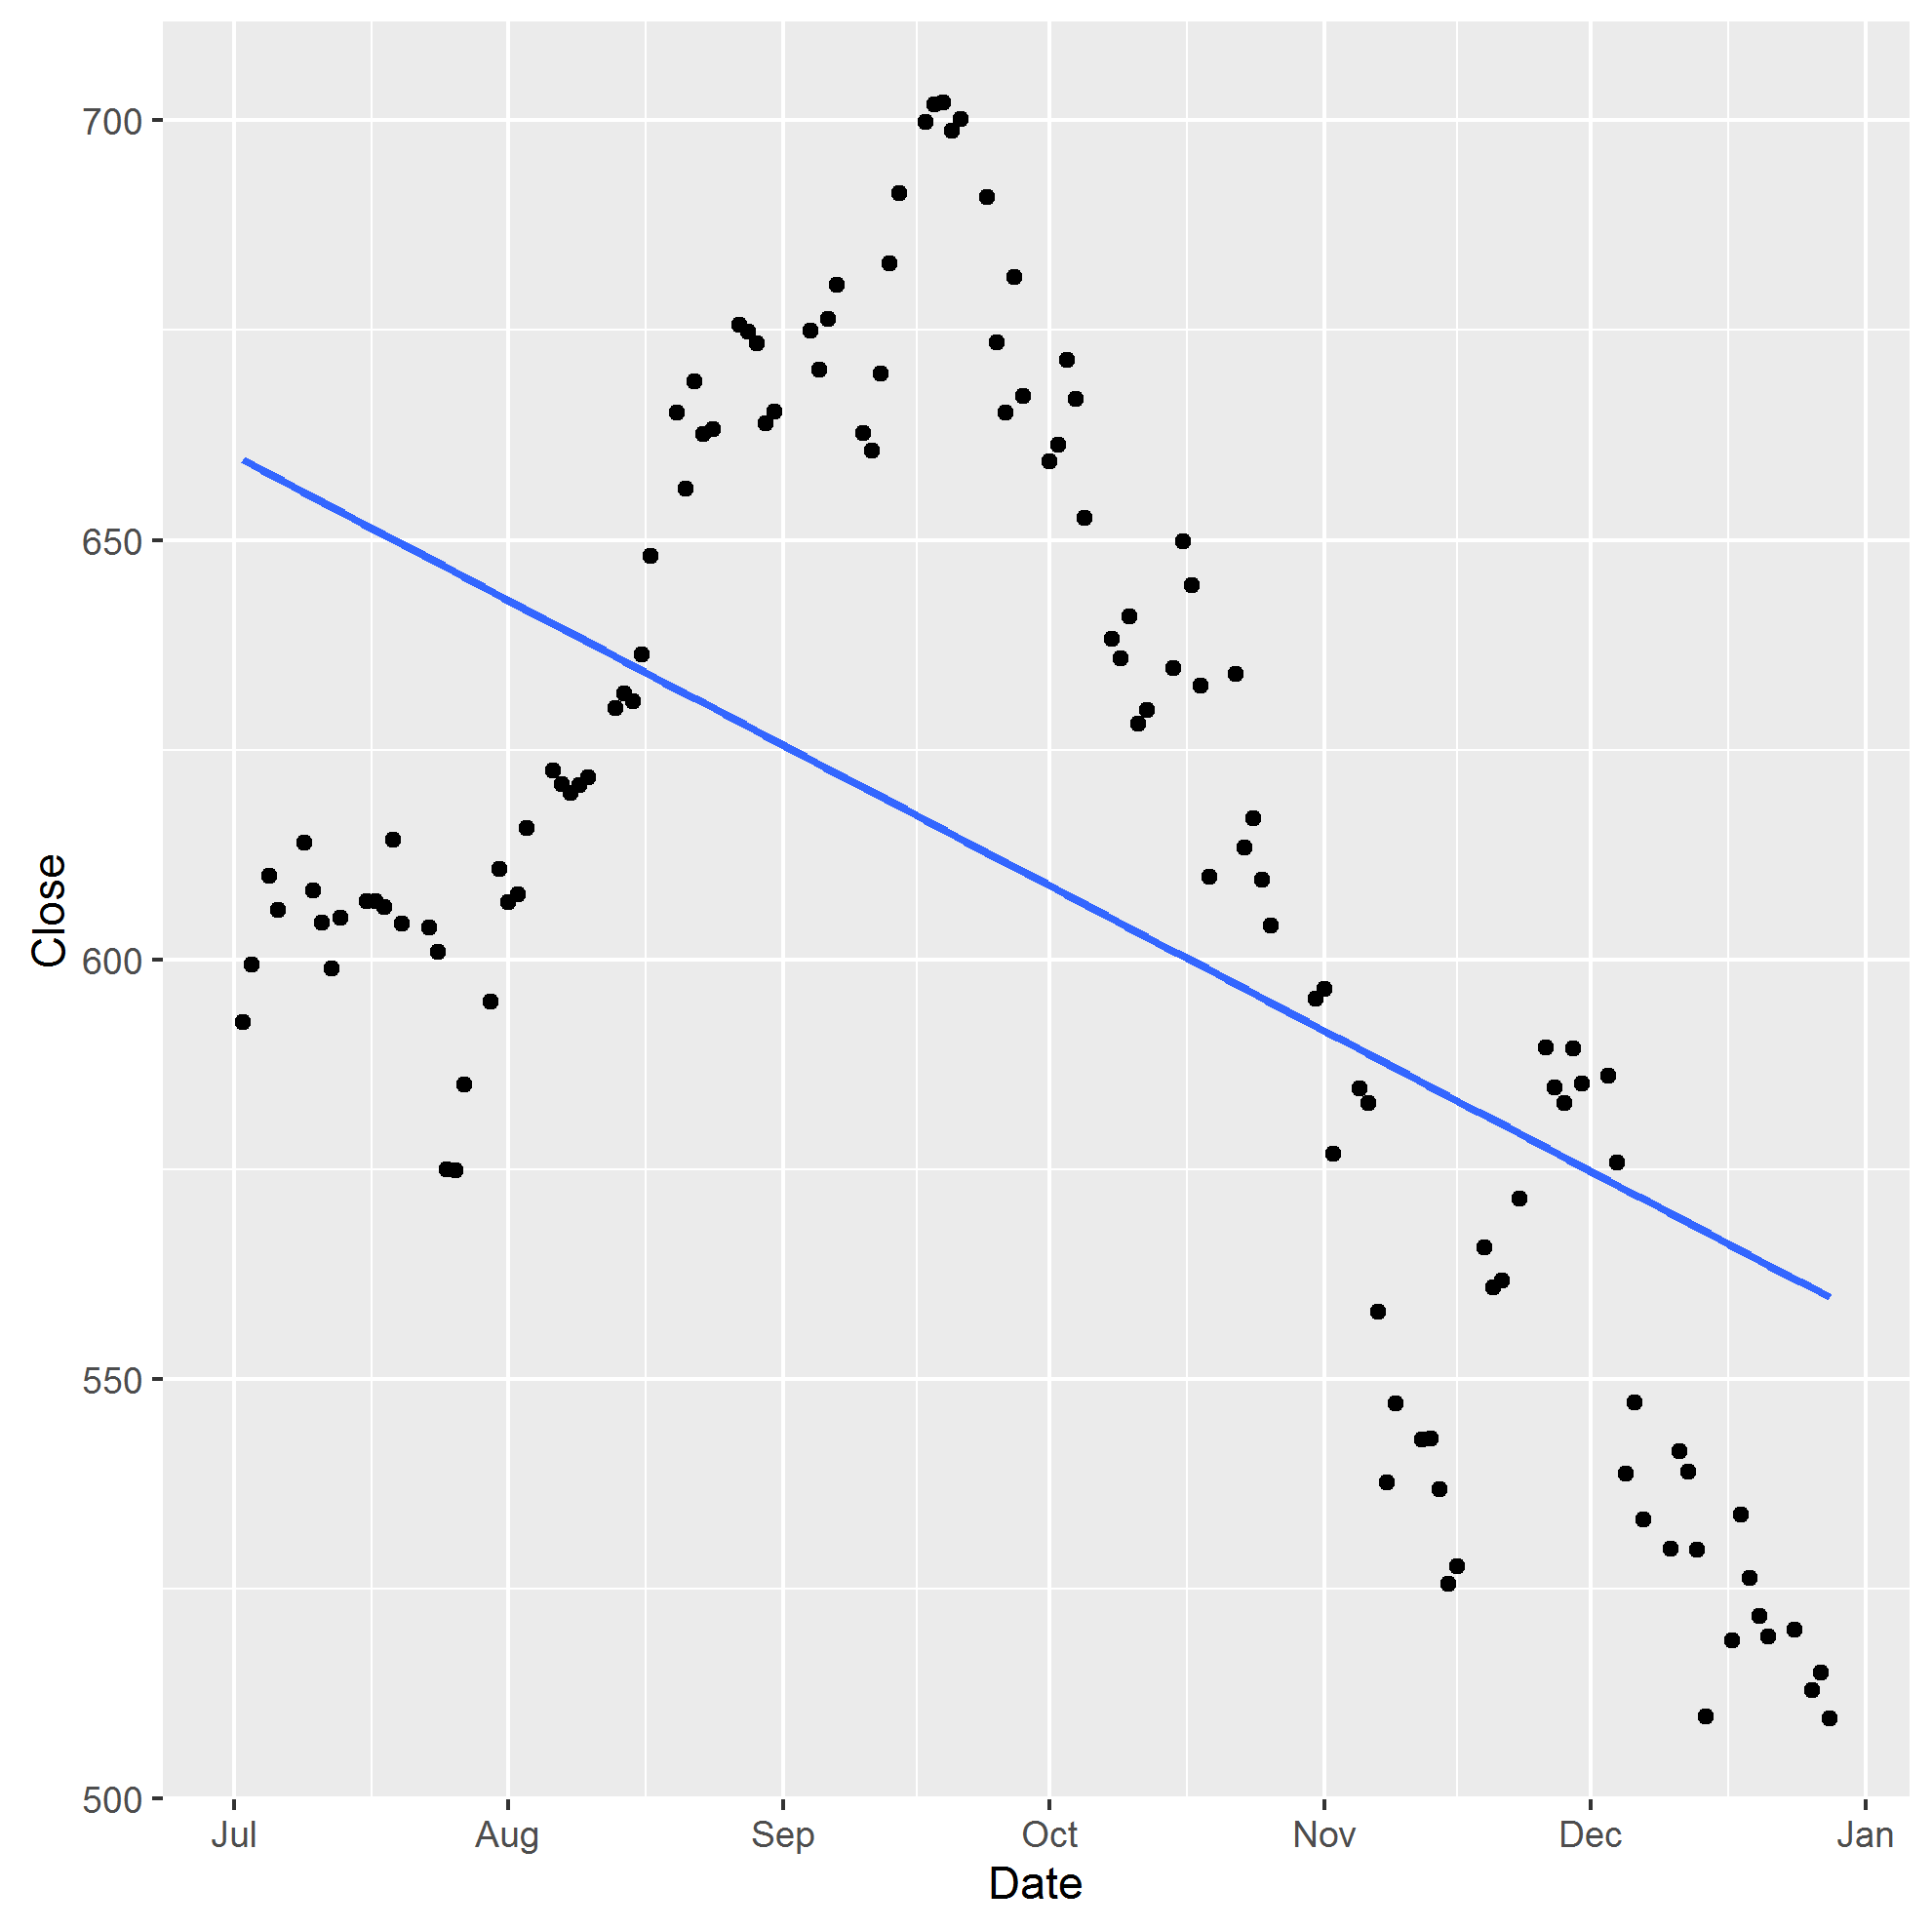
\includegraphics[width=\linewidth]{graph/a_reg4.png}
  \caption{Linear regression line of Apple closing prices.}
\endminipage\hfill
\minipage{0.46\textwidth}
  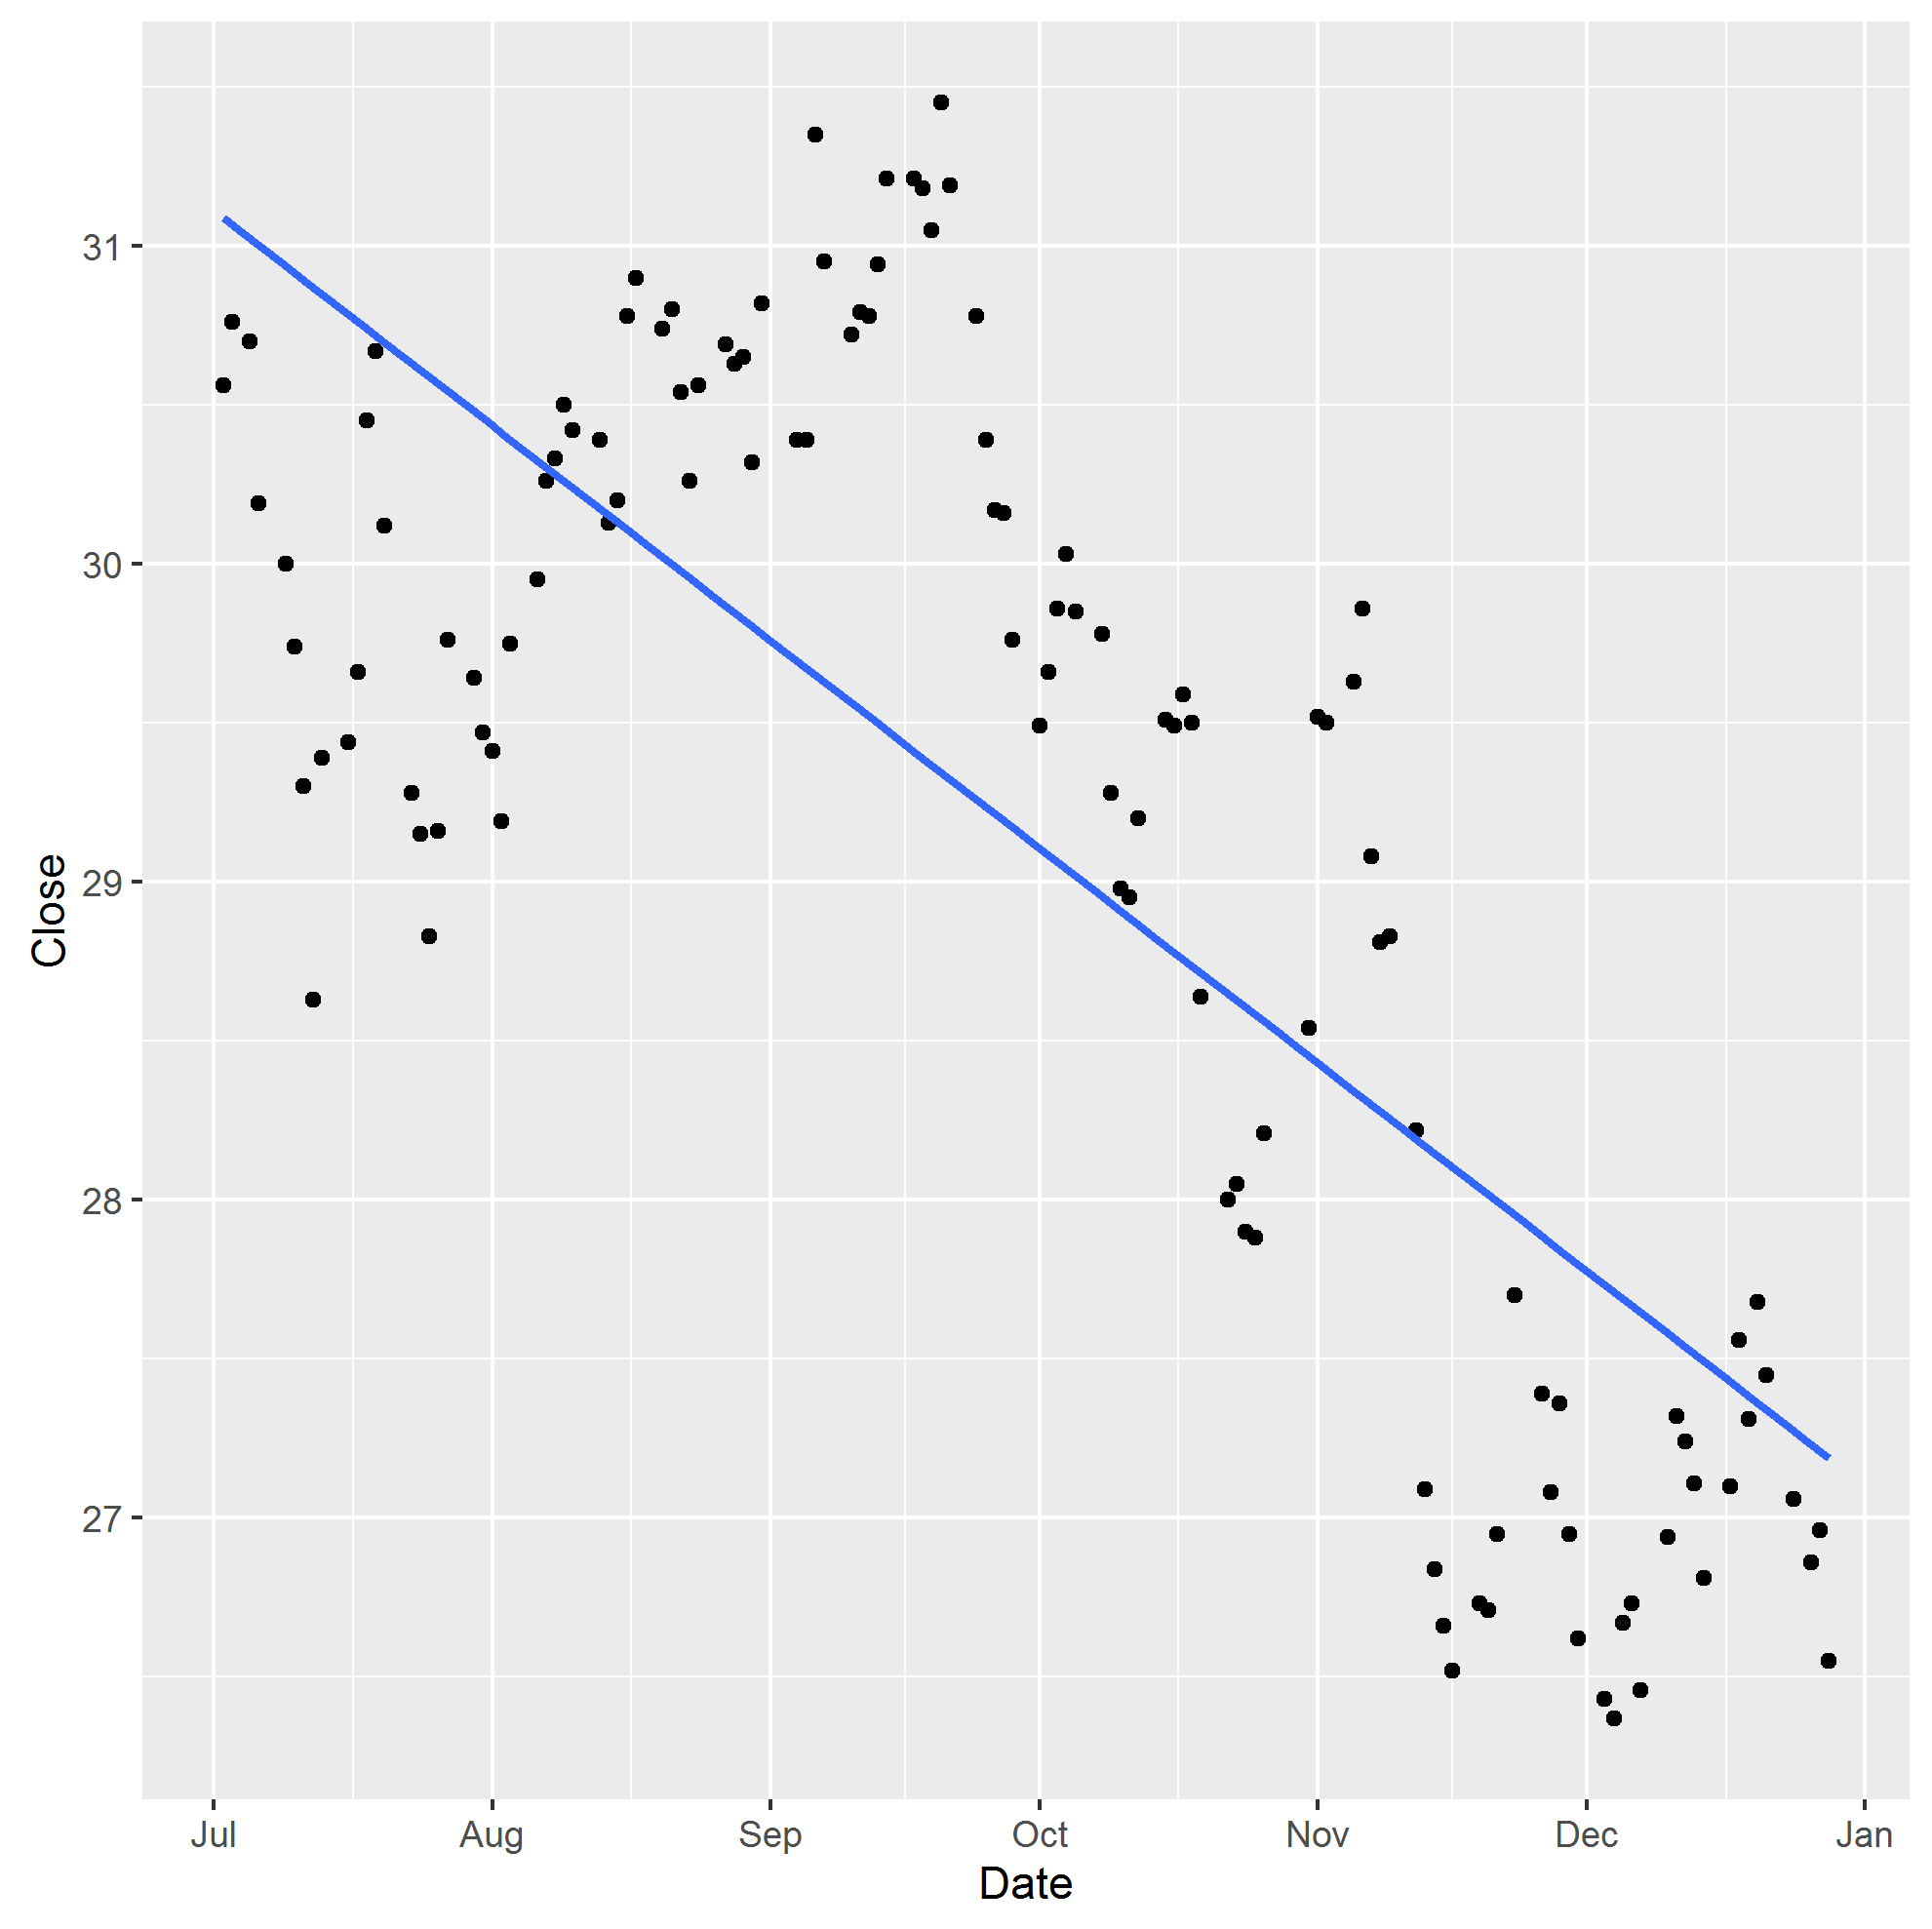
\includegraphics[width=\linewidth]{graph/m_reg4.png}
  \caption{Linear regression line of Microsoft closing prices.}
\endminipage\hfill
\end{figure}

Discuss regression lines. 

List y intercept, slope overall. 

\begin{figure}[!htb]
\minipage{0.46\textwidth}
  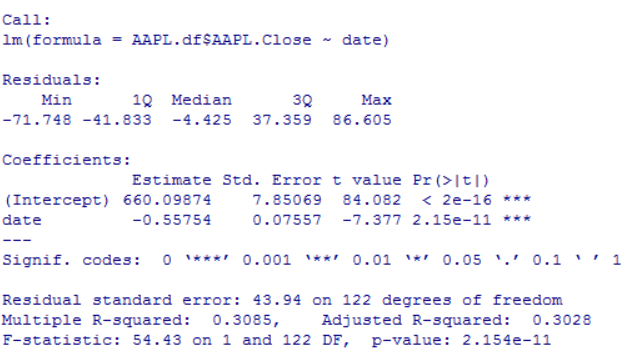
\includegraphics[width=\linewidth]{graph/aapl_reg_4.png}
  \caption{Linear regression line of Apple closing prices.}
\endminipage\hfill
\minipage{0.46\textwidth}
  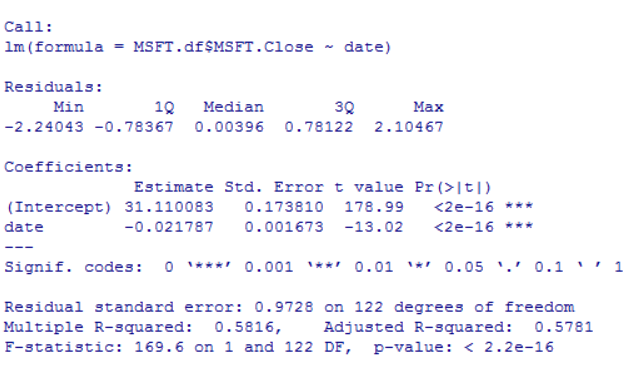
\includegraphics[width=\linewidth]{graph/msft_reg_4.png}
  \caption{Linear regression line of Microsoft closing prices.}
\endminipage\hfill
\end{figure}


\subsubsection{Analysis}
Discuss any interesting overall observations here


\subsection{January - June  2013 }
\subsubsection{Plots}
\begin{figure}[!htb]
\minipage{0.46\textwidth}
  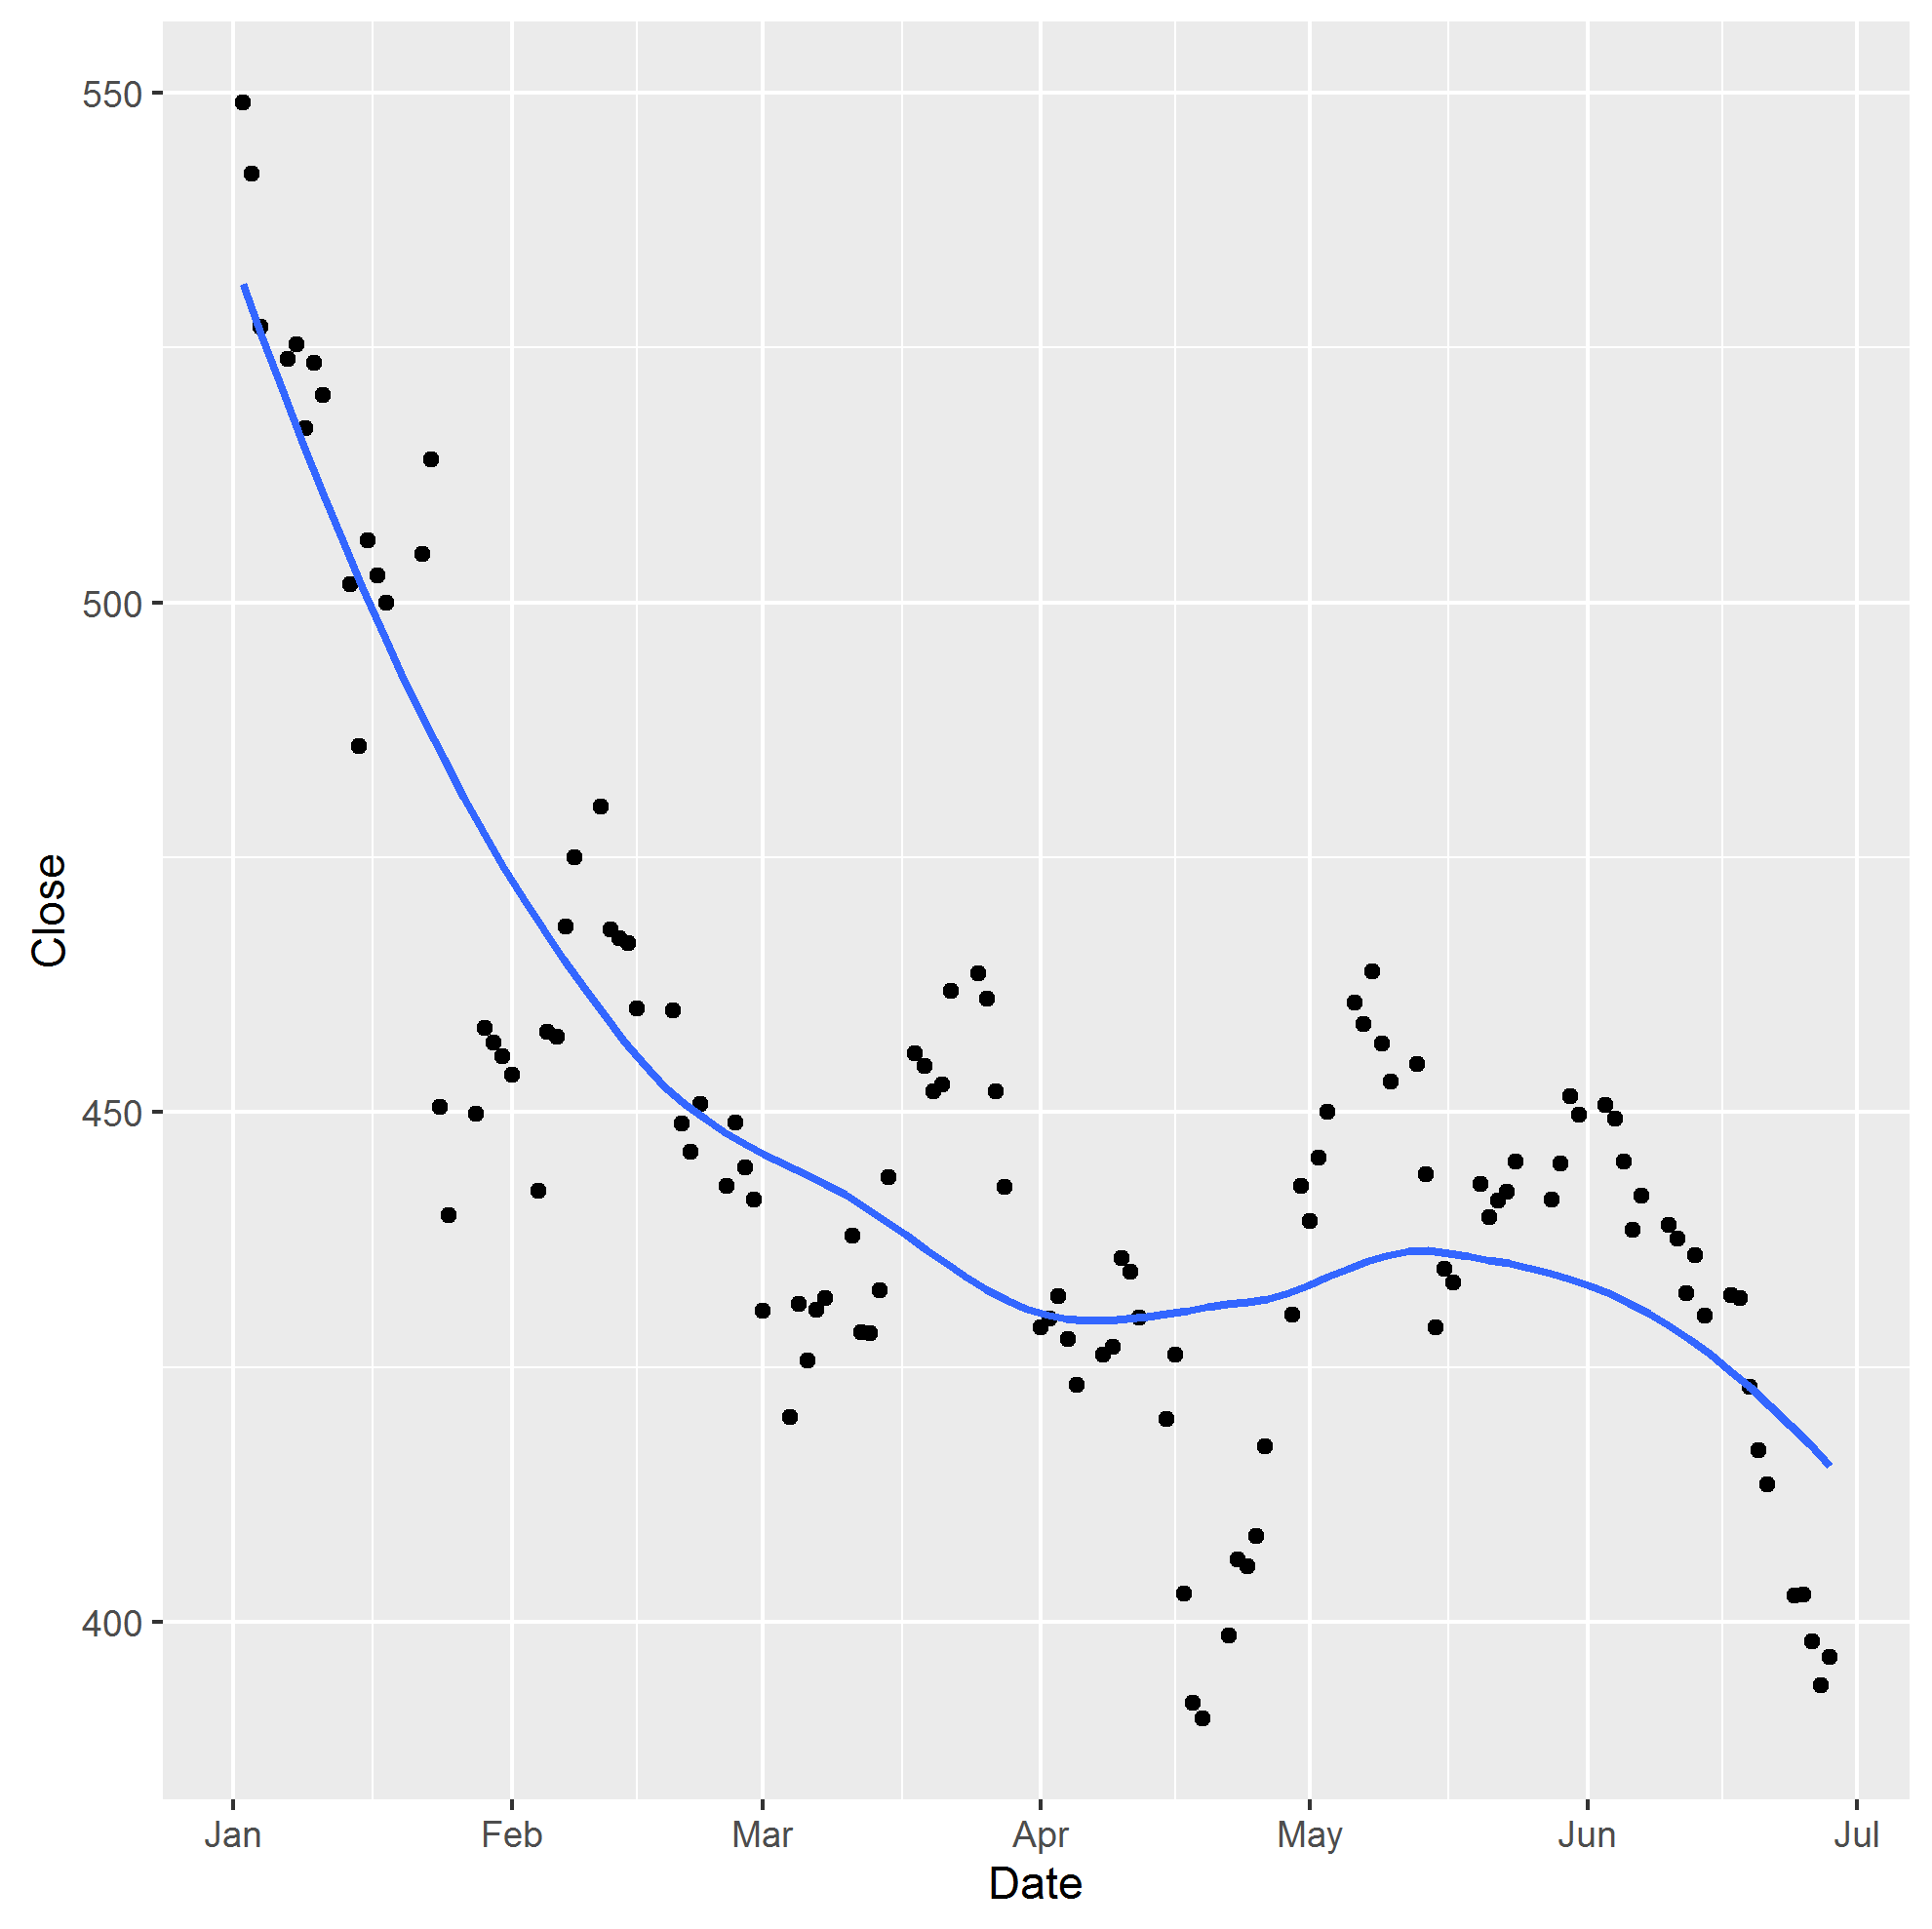
\includegraphics[width=\linewidth]{graph/AAPL5.png}
  \caption{Scatter plot with graph of Apple stock}
\endminipage\hfill
\minipage{0.46\textwidth}
  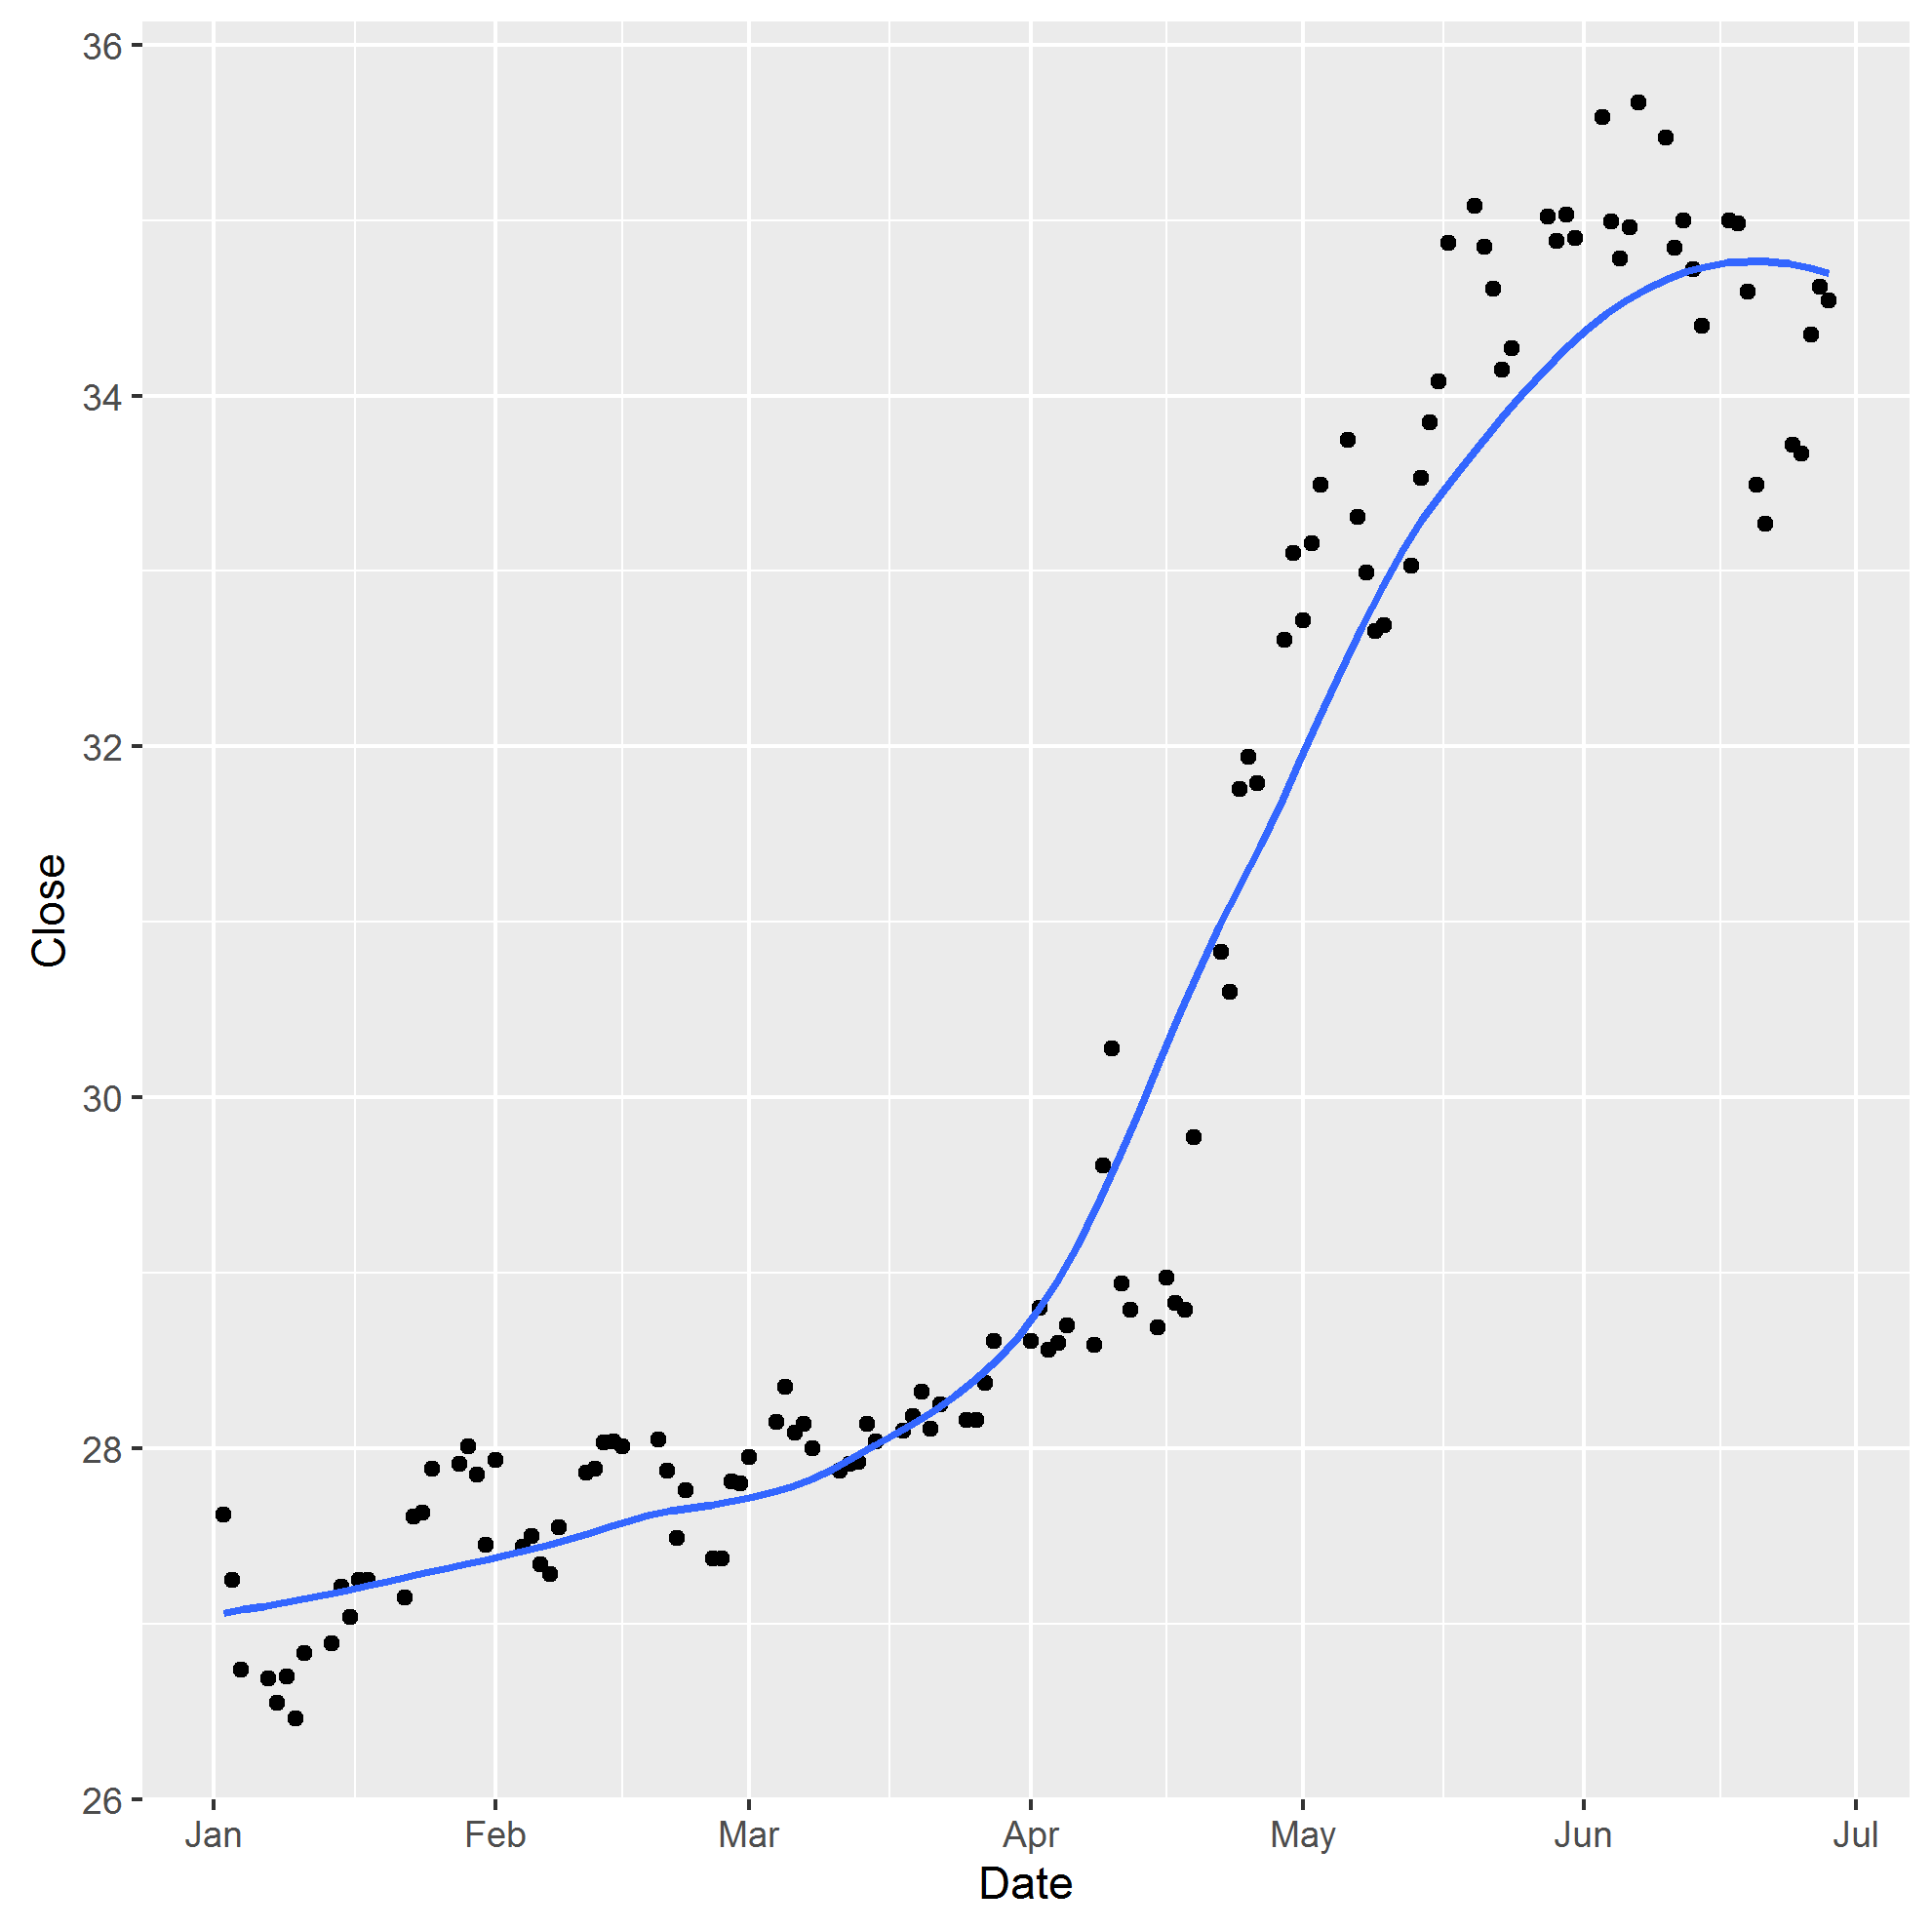
\includegraphics[width=\linewidth]{graph/MSFT5.png}
  \caption{Scatter plot with graph of Microsoft stock}
\endminipage\hfill

\end{figure}
\begin{enumerate}
\item {\bf Apple chart}
\end{enumerate}
\subsubsection{Correlation}

\begin{figure}[!htb]
\minipage{0.8\textwidth}
  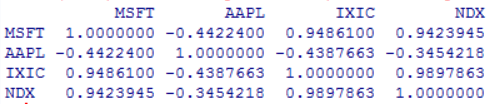
\includegraphics[width=\linewidth]{graph/cor5.png}
  \caption{Correlation table for Microsoft and Apple against two index stocks}
\endminipage\hfill
\end{figure}

Insert correlation table MS vs apple
Discuss any interesting overall observations here

\subsubsection{Regression}
Show regression lines for MS and apple. 


\begin{figure}[!htb]
\minipage{0.46\textwidth}
  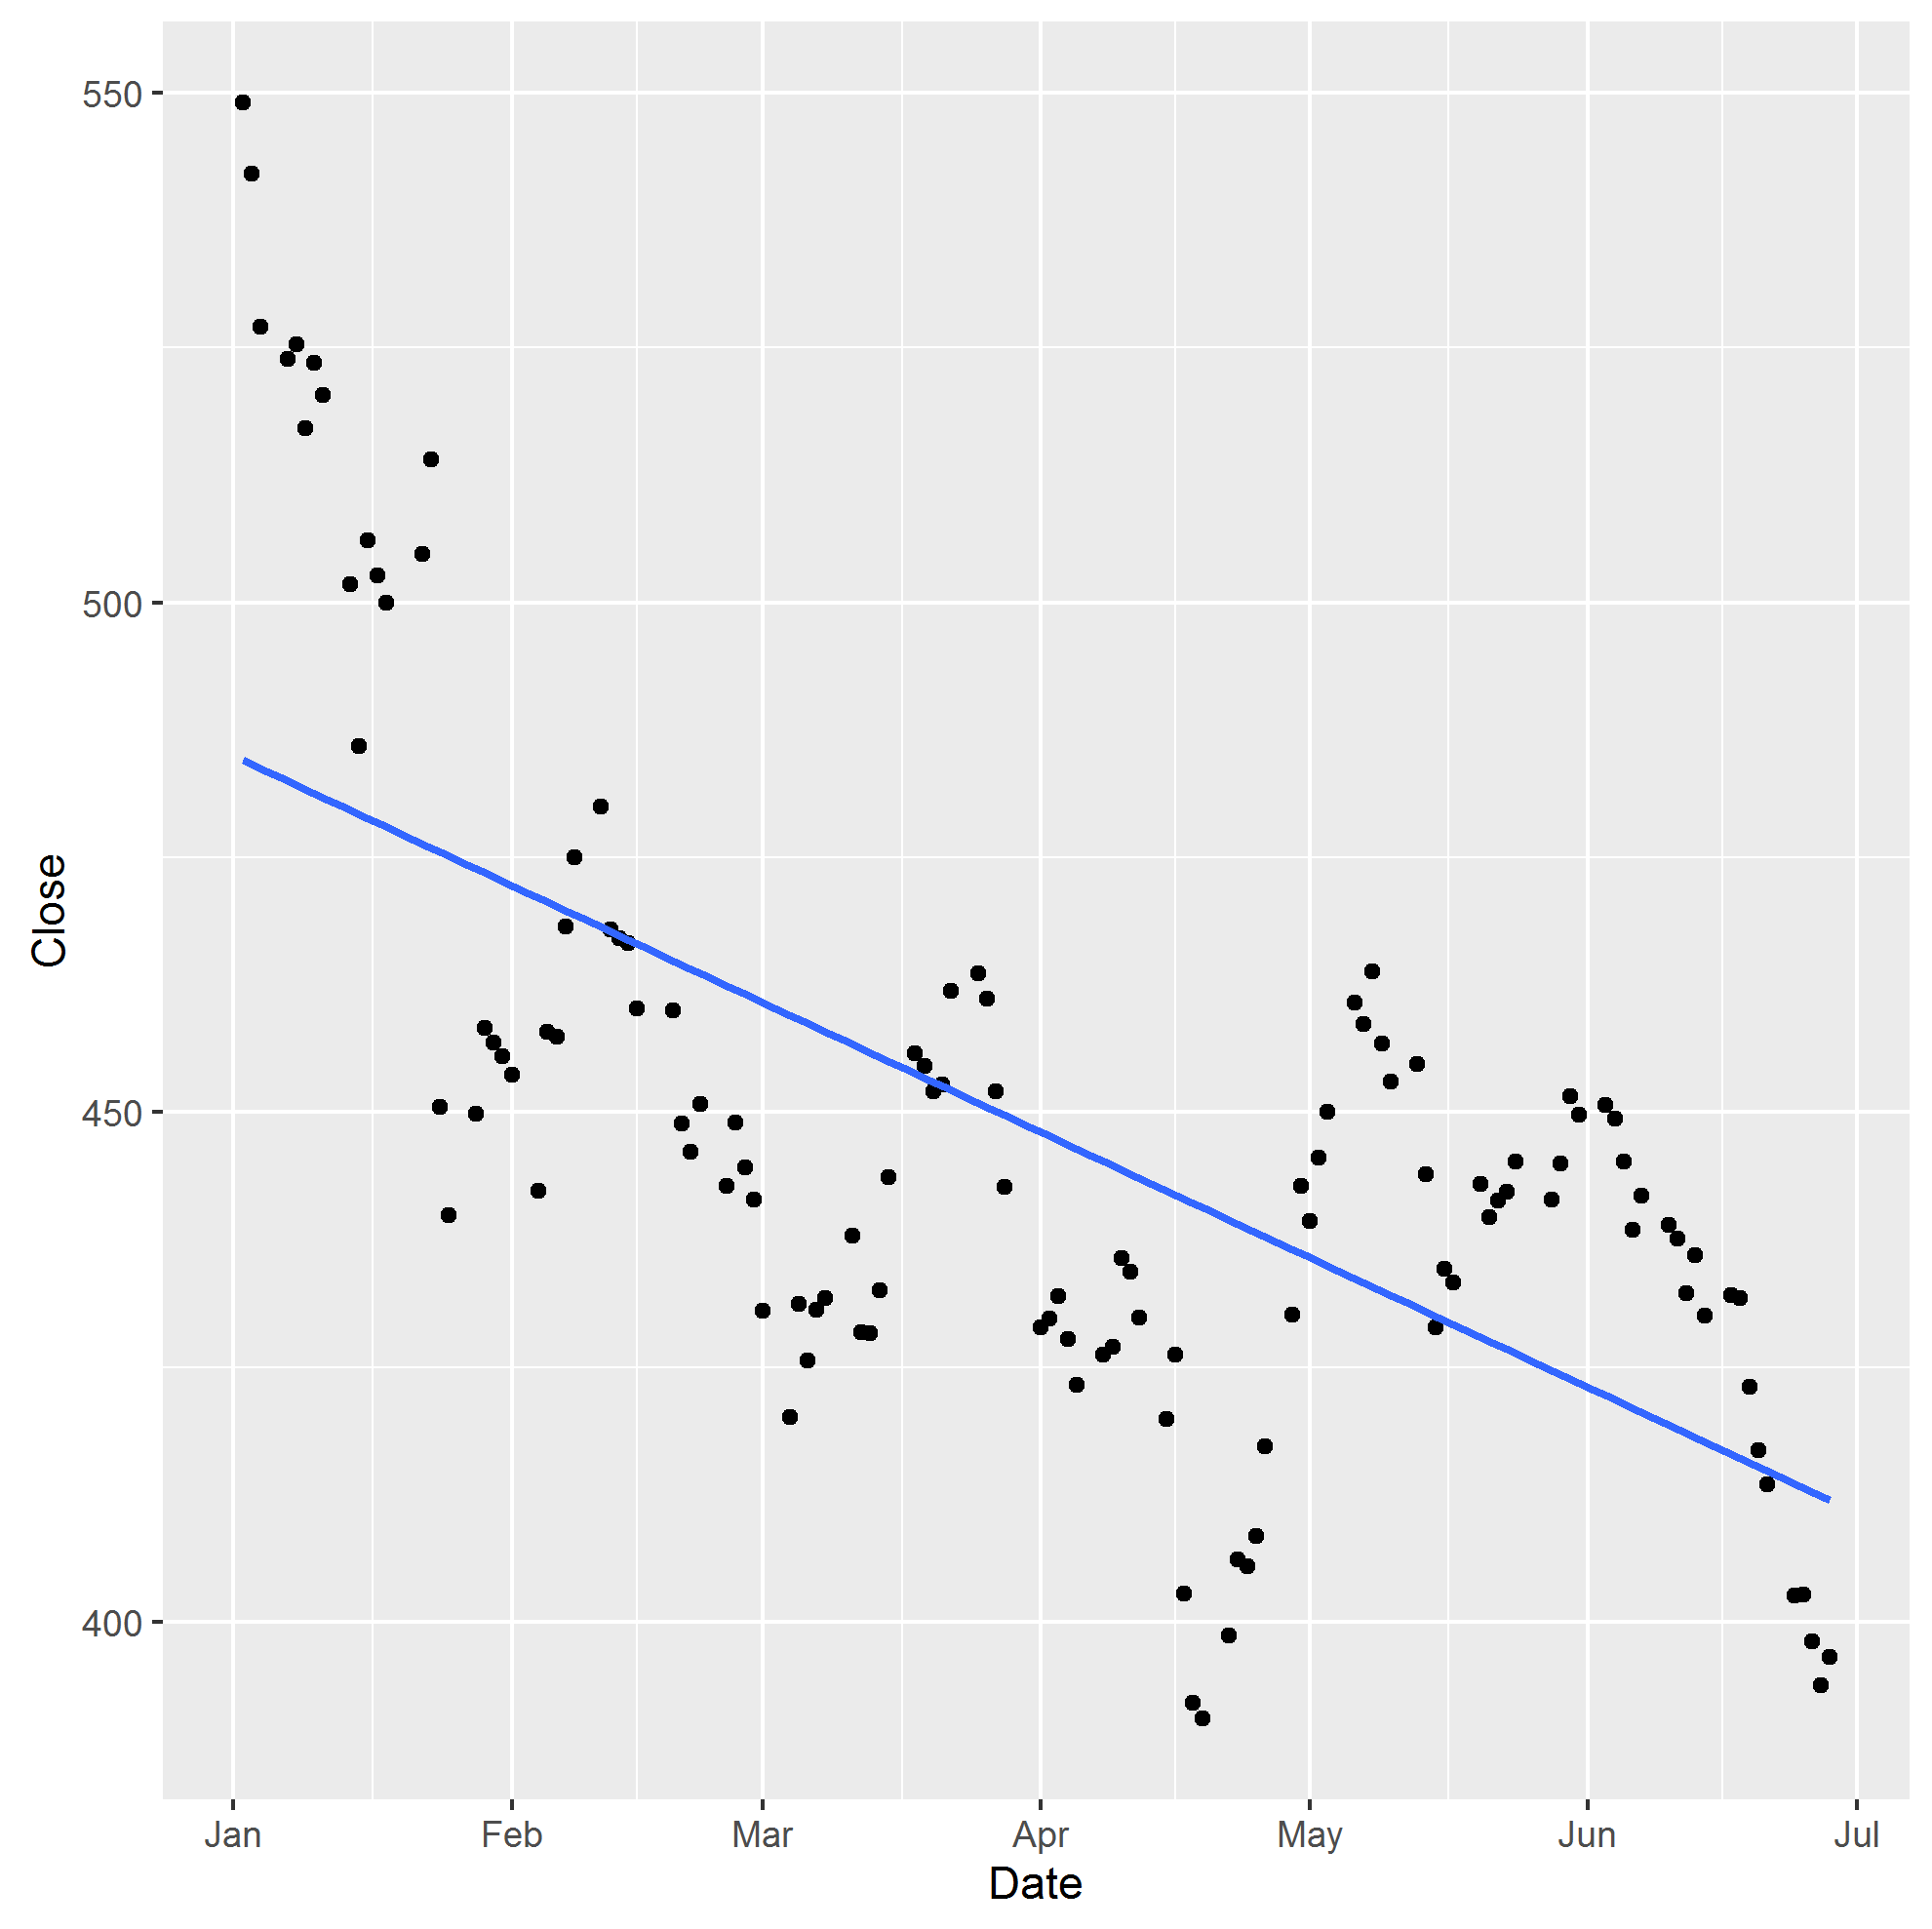
\includegraphics[width=\linewidth]{graph/a_reg5.png}
  \caption{Linear regression line of Apple closing prices.}
\endminipage\hfill
\minipage{0.46\textwidth}
  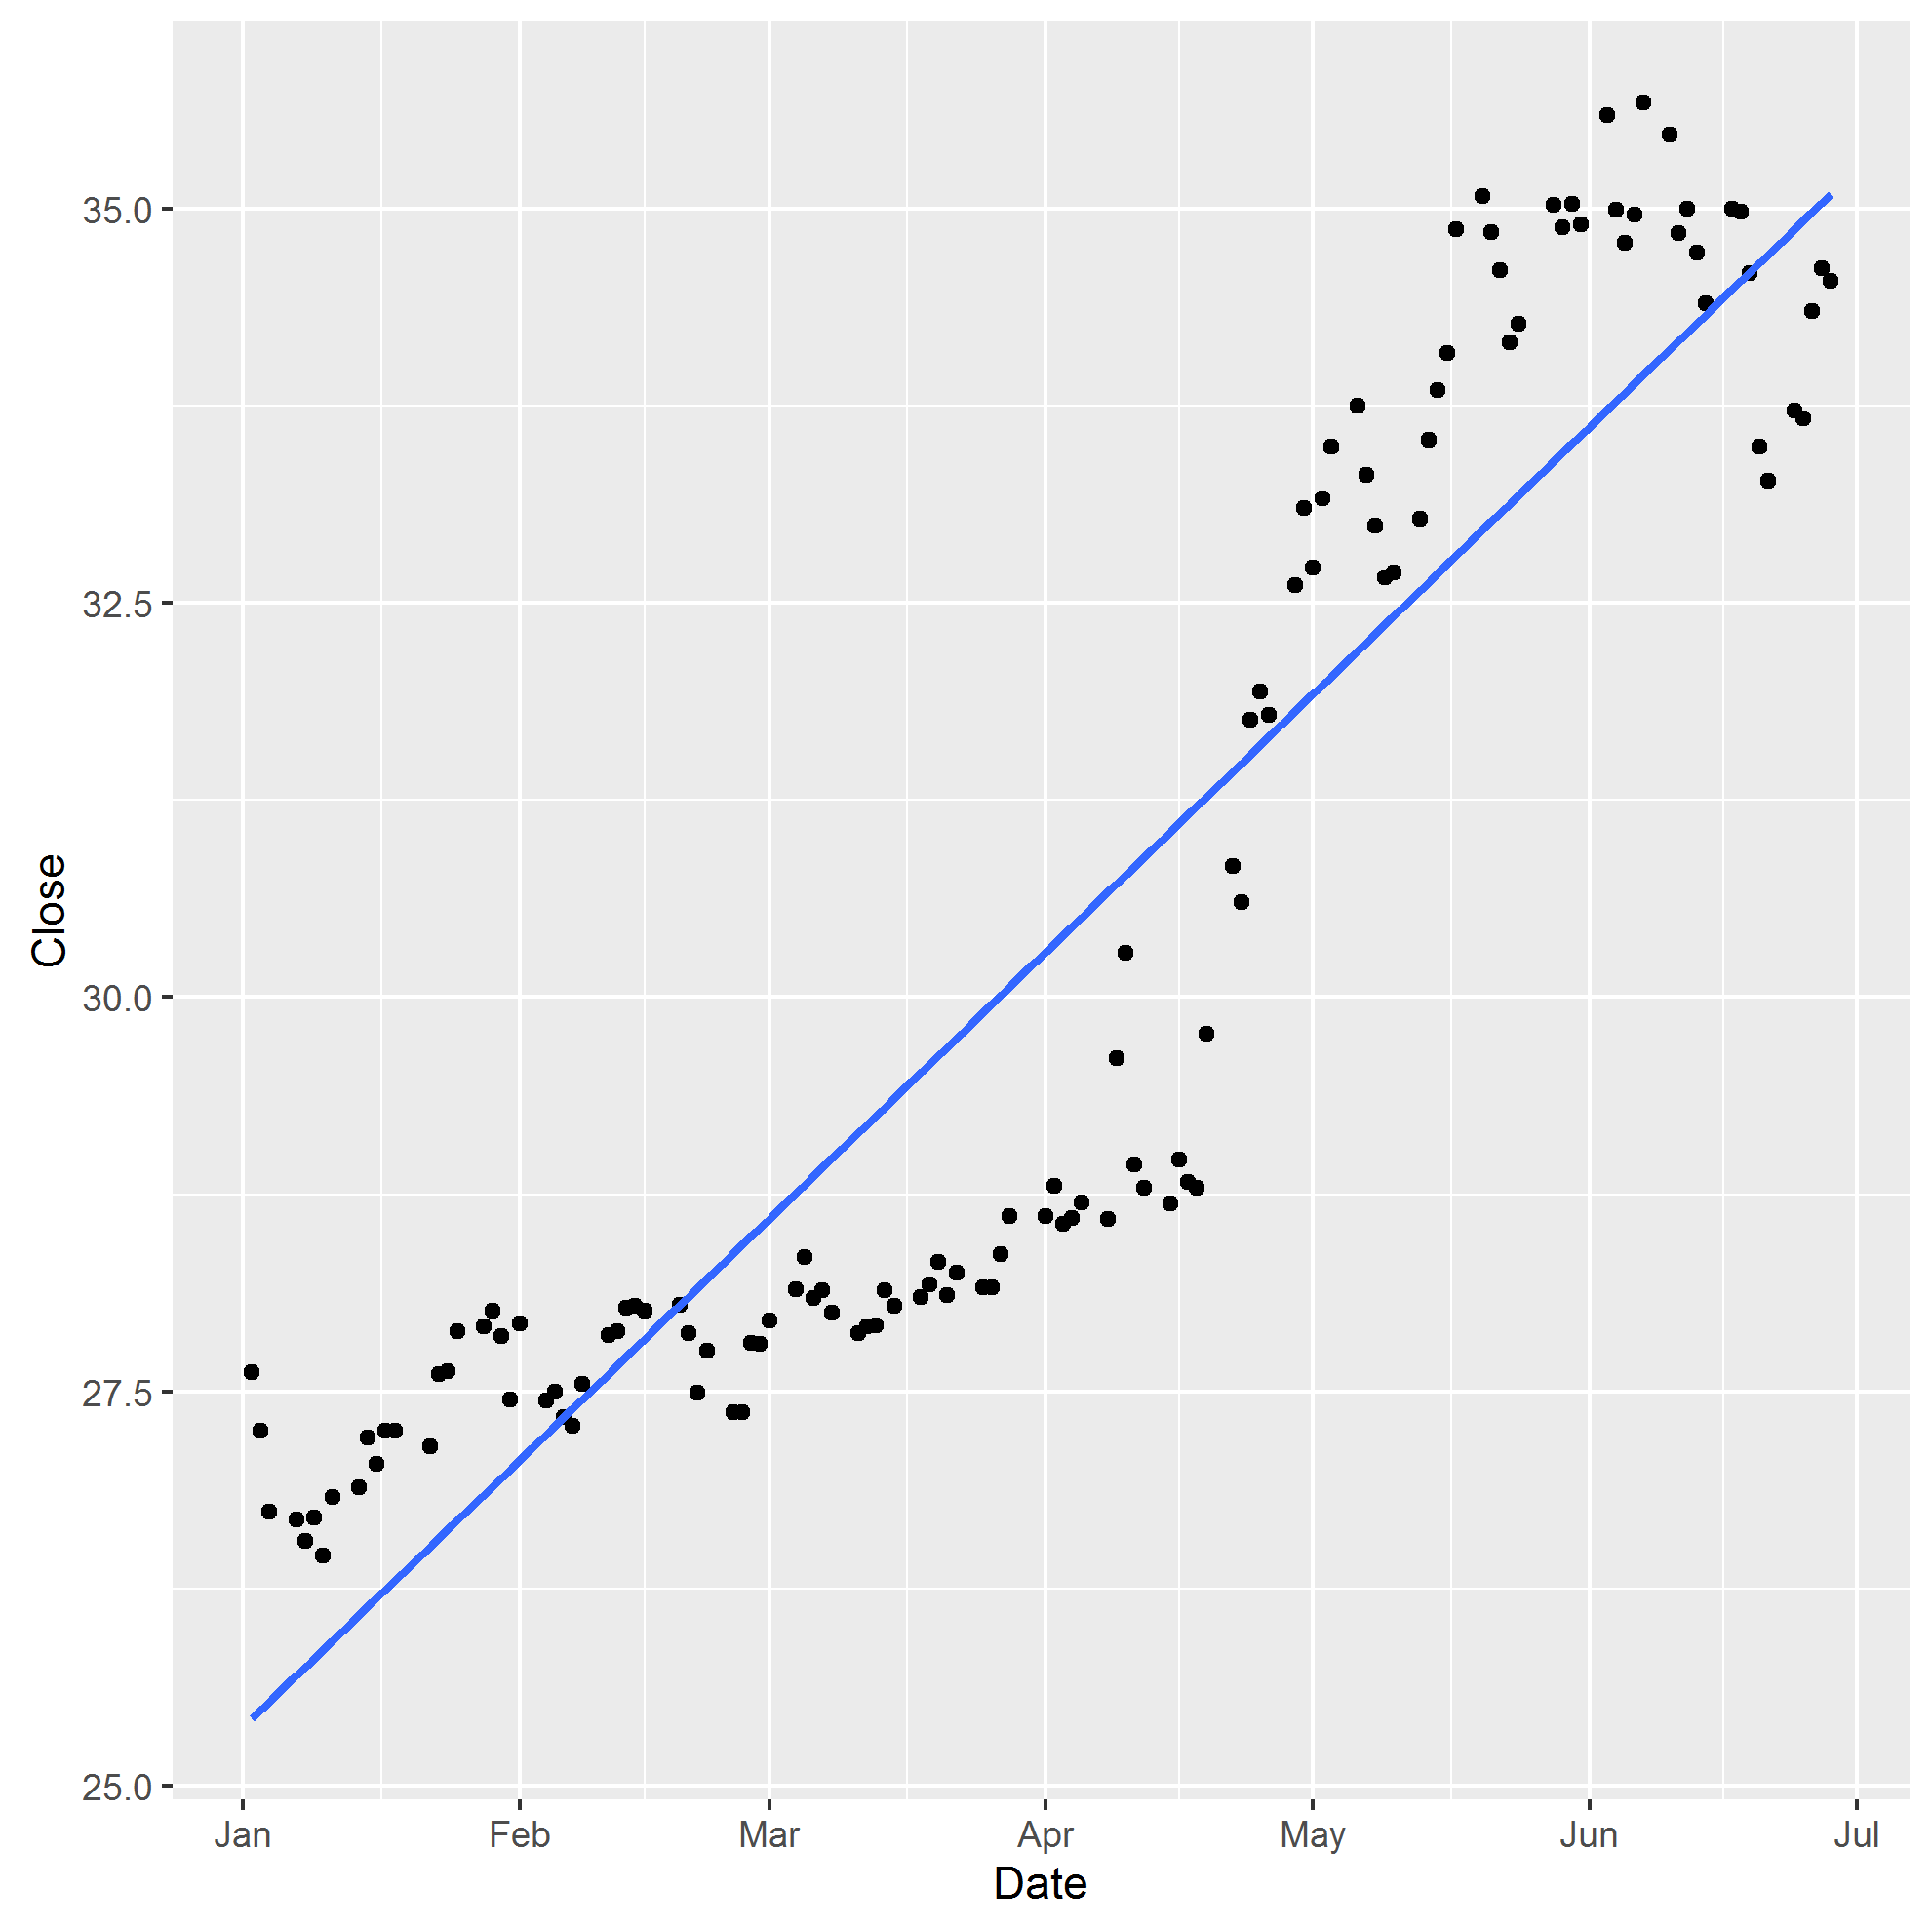
\includegraphics[width=\linewidth]{graph/m_reg5.png}
  \caption{Linear regression line of Microsoft closing prices.}
\endminipage\hfill
\end{figure}

Discuss regression lines. 

List y intercept, slope overall. 

\begin{figure}[!htb]
\minipage{0.46\textwidth}
  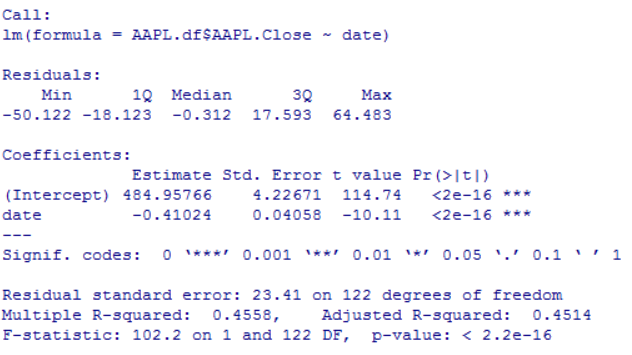
\includegraphics[width=\linewidth]{graph/aapl_reg_5.png}
  \caption{Linear regression line of Apple closing prices.}
\endminipage\hfill
\minipage{0.46\textwidth}
  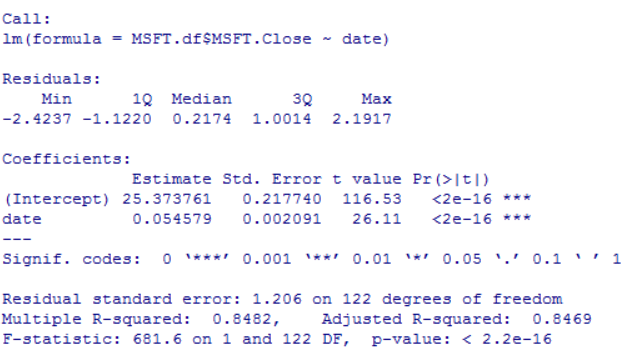
\includegraphics[width=\linewidth]{graph/msft_reg_5.png}
  \caption{Linear regression line of Microsoft closing prices.}
\endminipage\hfill
\end{figure}


\subsubsection{Analysis}
Discuss any interesting observations here.

\subsection{July - December  2013 }
\subsubsection{Plots}
\begin{figure}[!htb]
\minipage{0.46\textwidth}
  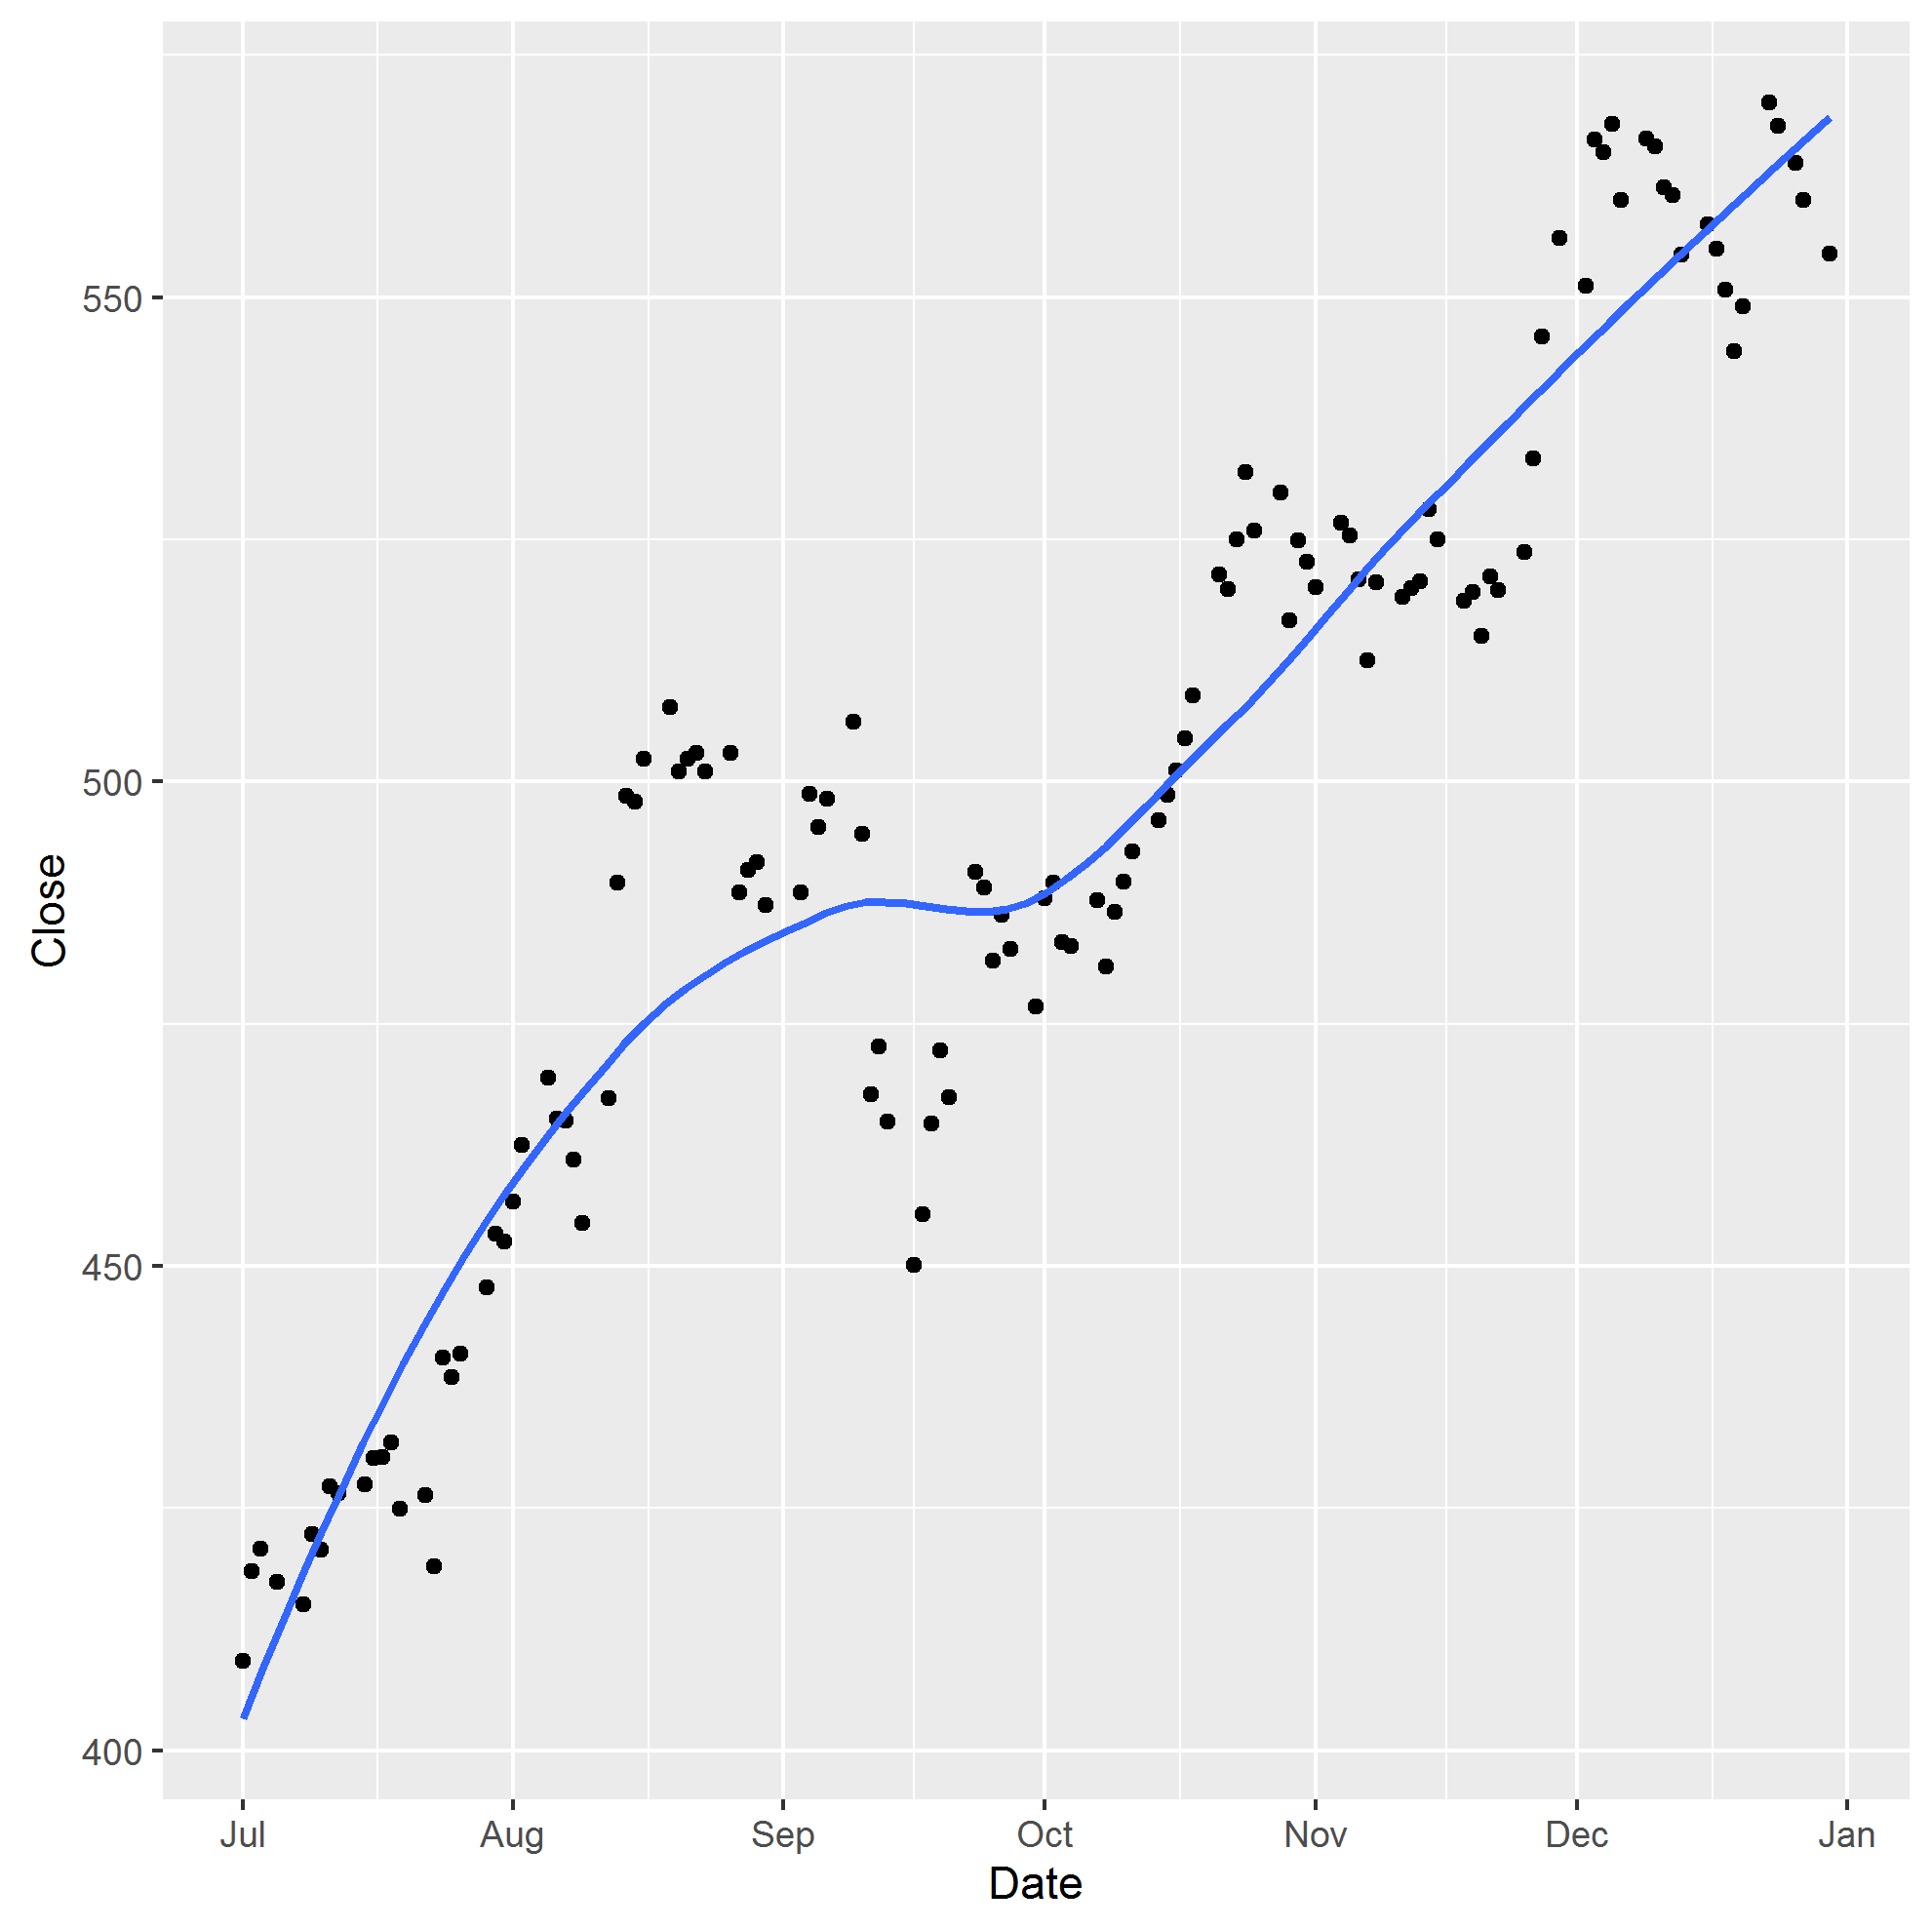
\includegraphics[width=\linewidth]{graph/AAPL6.png}
  \caption{Scatter plot with graph of Apple stock}
\endminipage\hfill
\minipage{0.46\textwidth}
  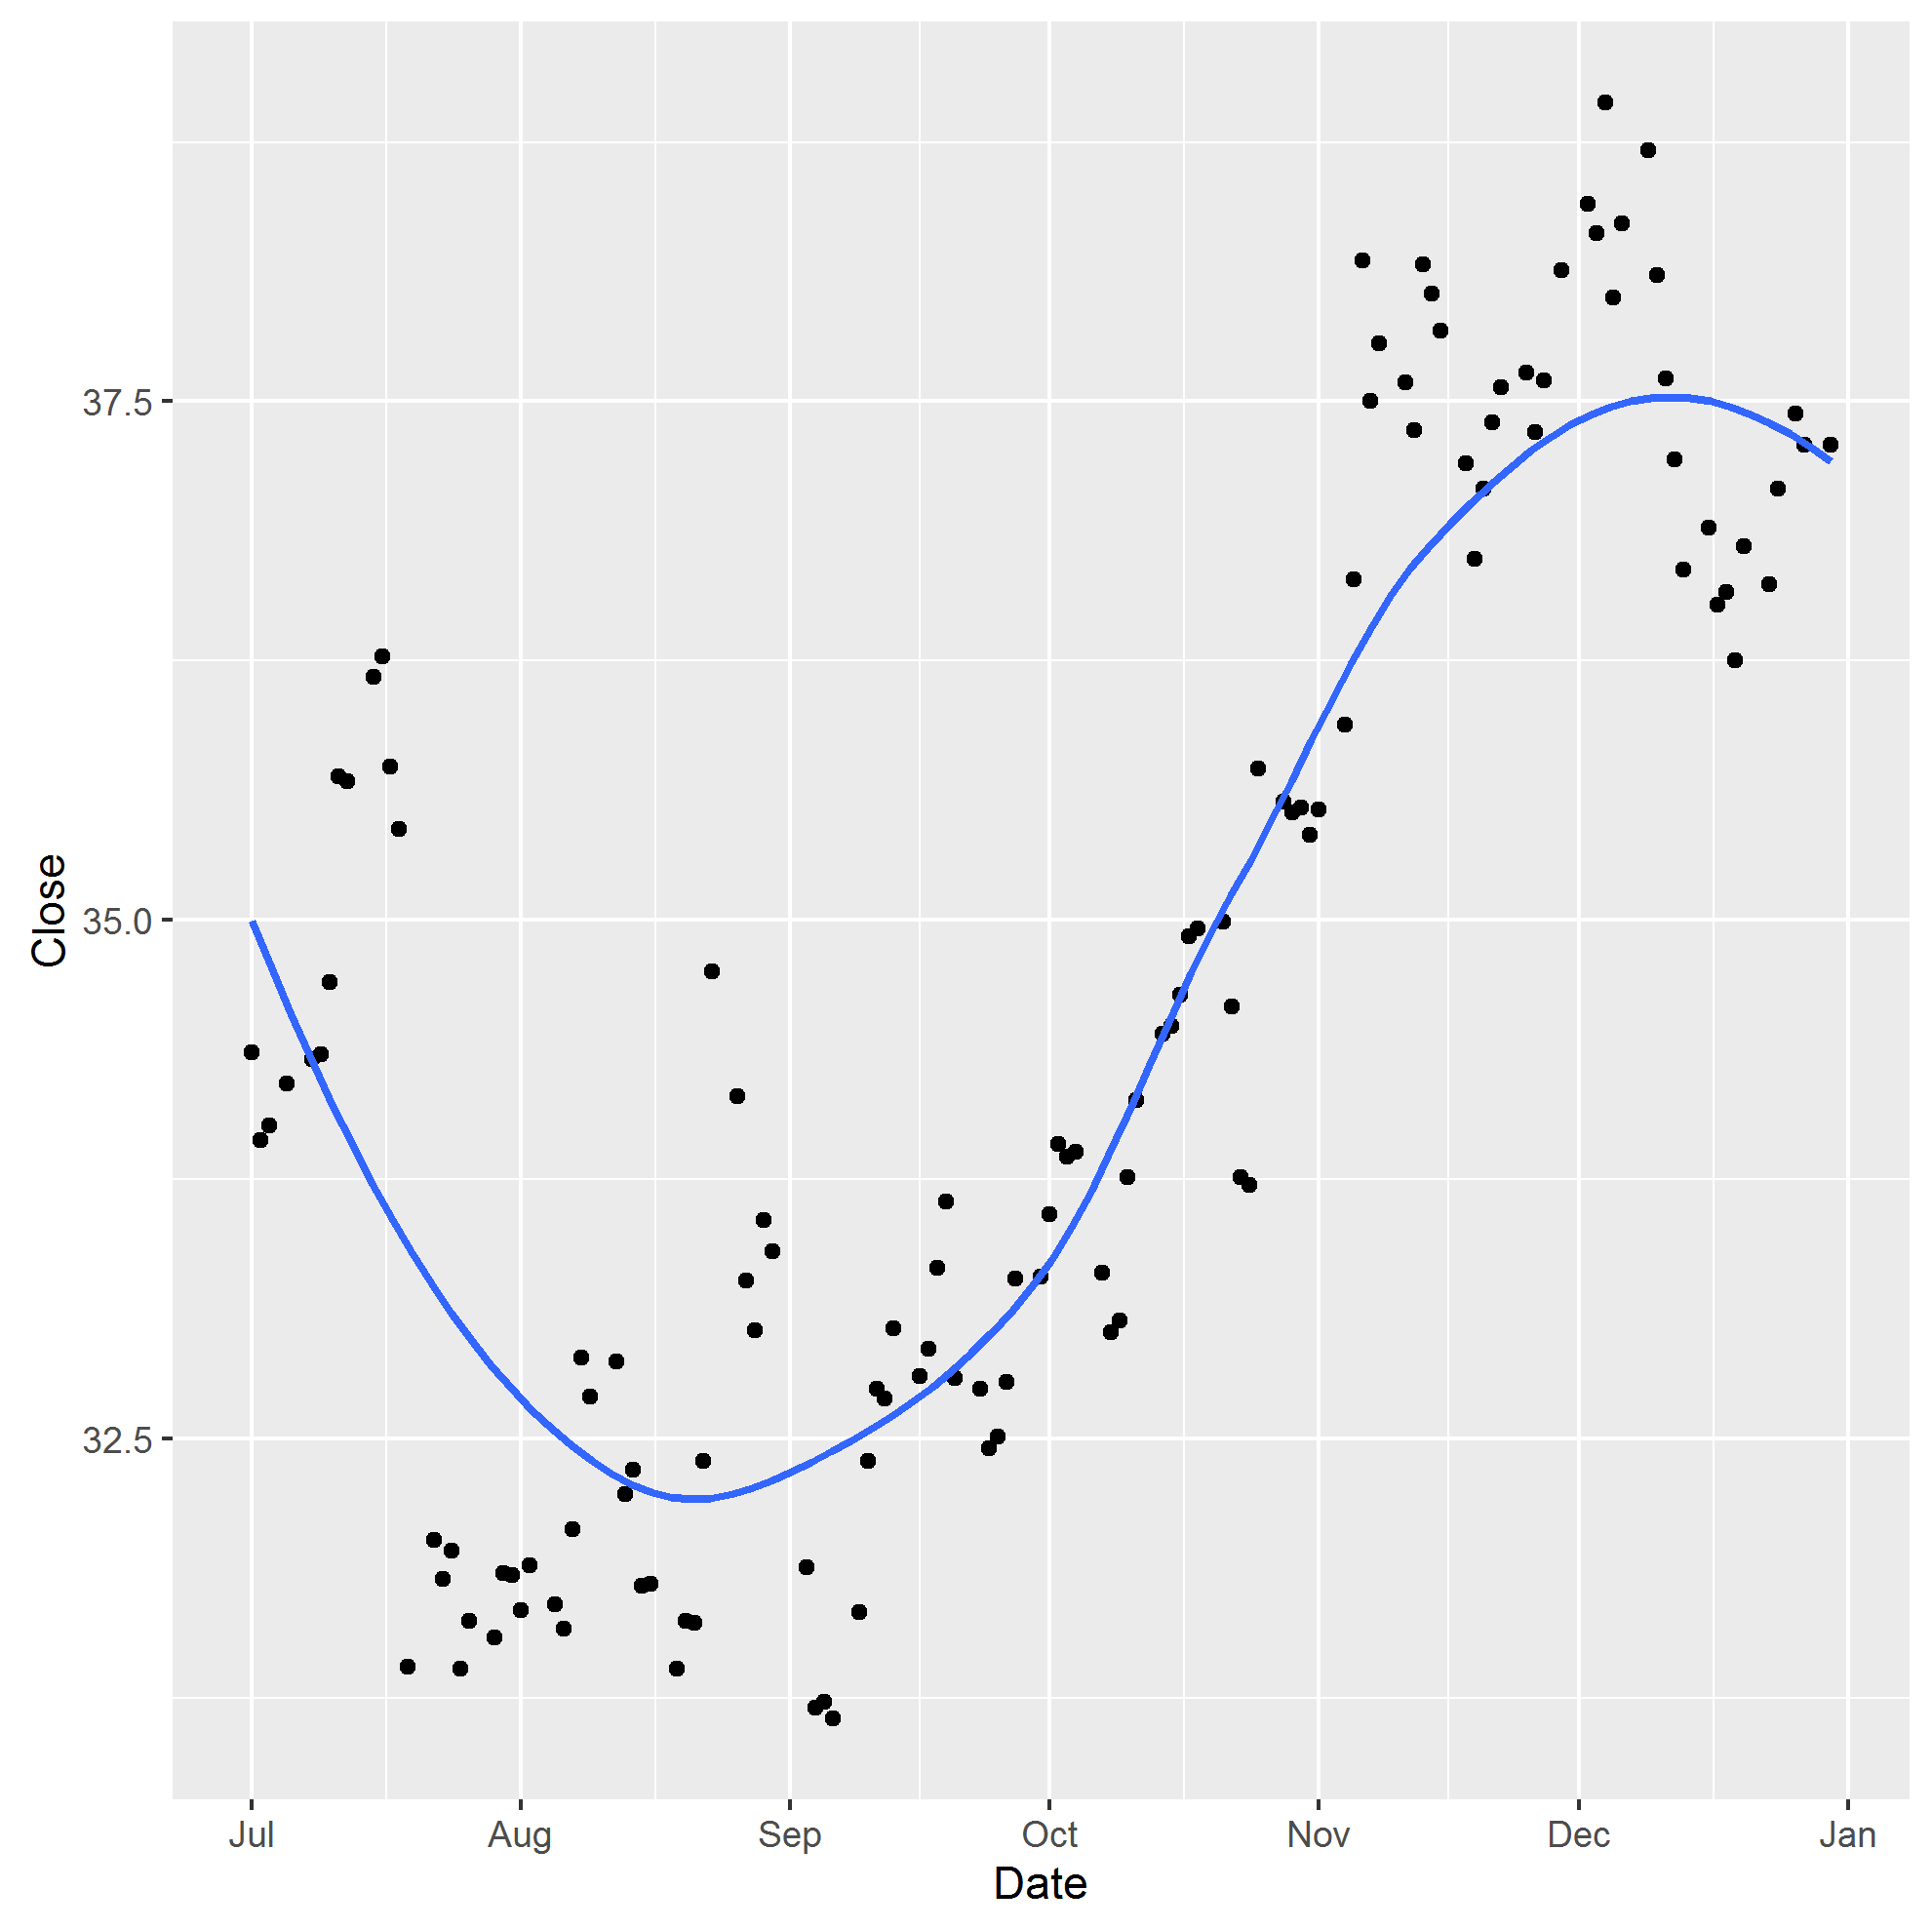
\includegraphics[width=\linewidth]{graph/MSFT6.png}
  \caption{Scatter plot with graph of Microsoft stock}
\endminipage\hfill

\end{figure}
Discuss apple chart
Discuss Microsoft chart
\subsubsection{Correlation}

\begin{figure}[!htb]
\minipage{0.8\textwidth}
  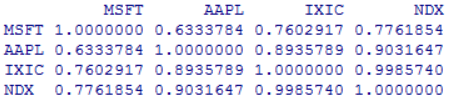
\includegraphics[width=\linewidth]{graph/cor6.png}
  \caption{Correlation table for Microsoft and Apple against two index stocks}
\endminipage\hfill
\end{figure}

Insert correlation table MS vs apple
Discuss any interesting overall observations here

\subsubsection{Regression}
Show regression lines for MS and apple. 


\begin{figure}[!htb]
\minipage{0.46\textwidth}
  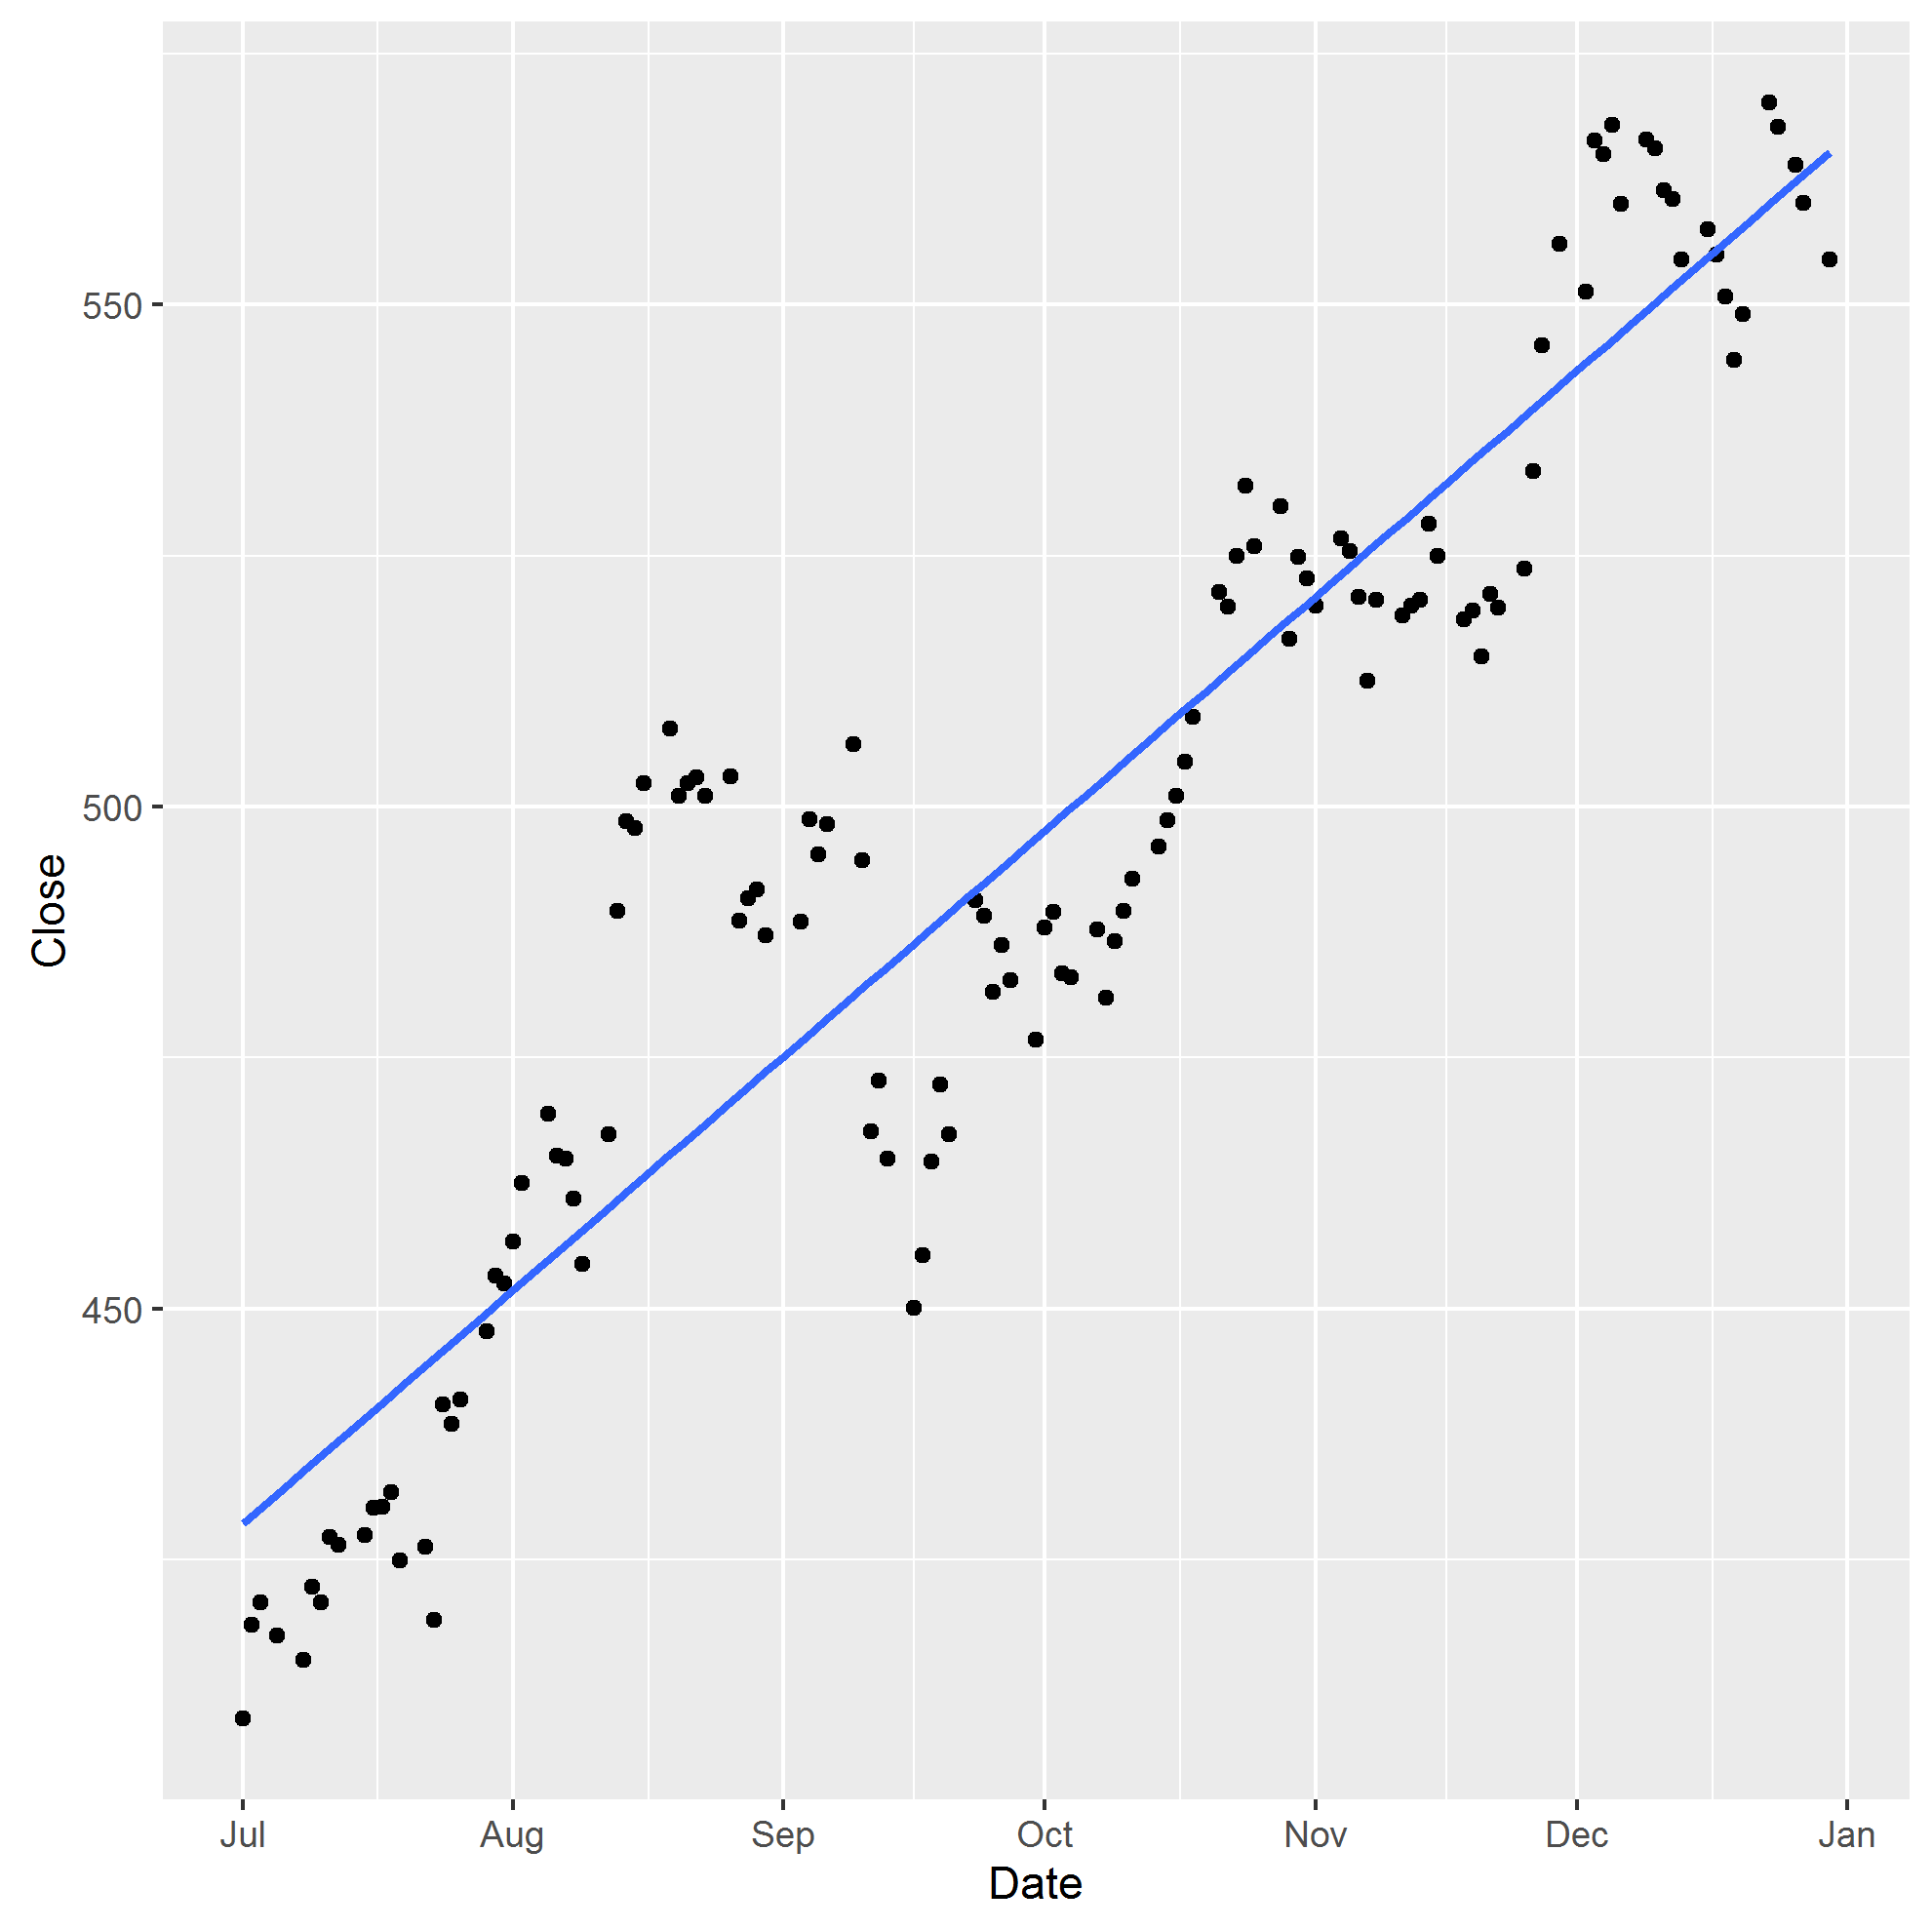
\includegraphics[width=\linewidth]{graph/a_reg6.png}
  \caption{Linear regression line of Apple closing prices.}
\endminipage\hfill
\minipage{0.46\textwidth}
  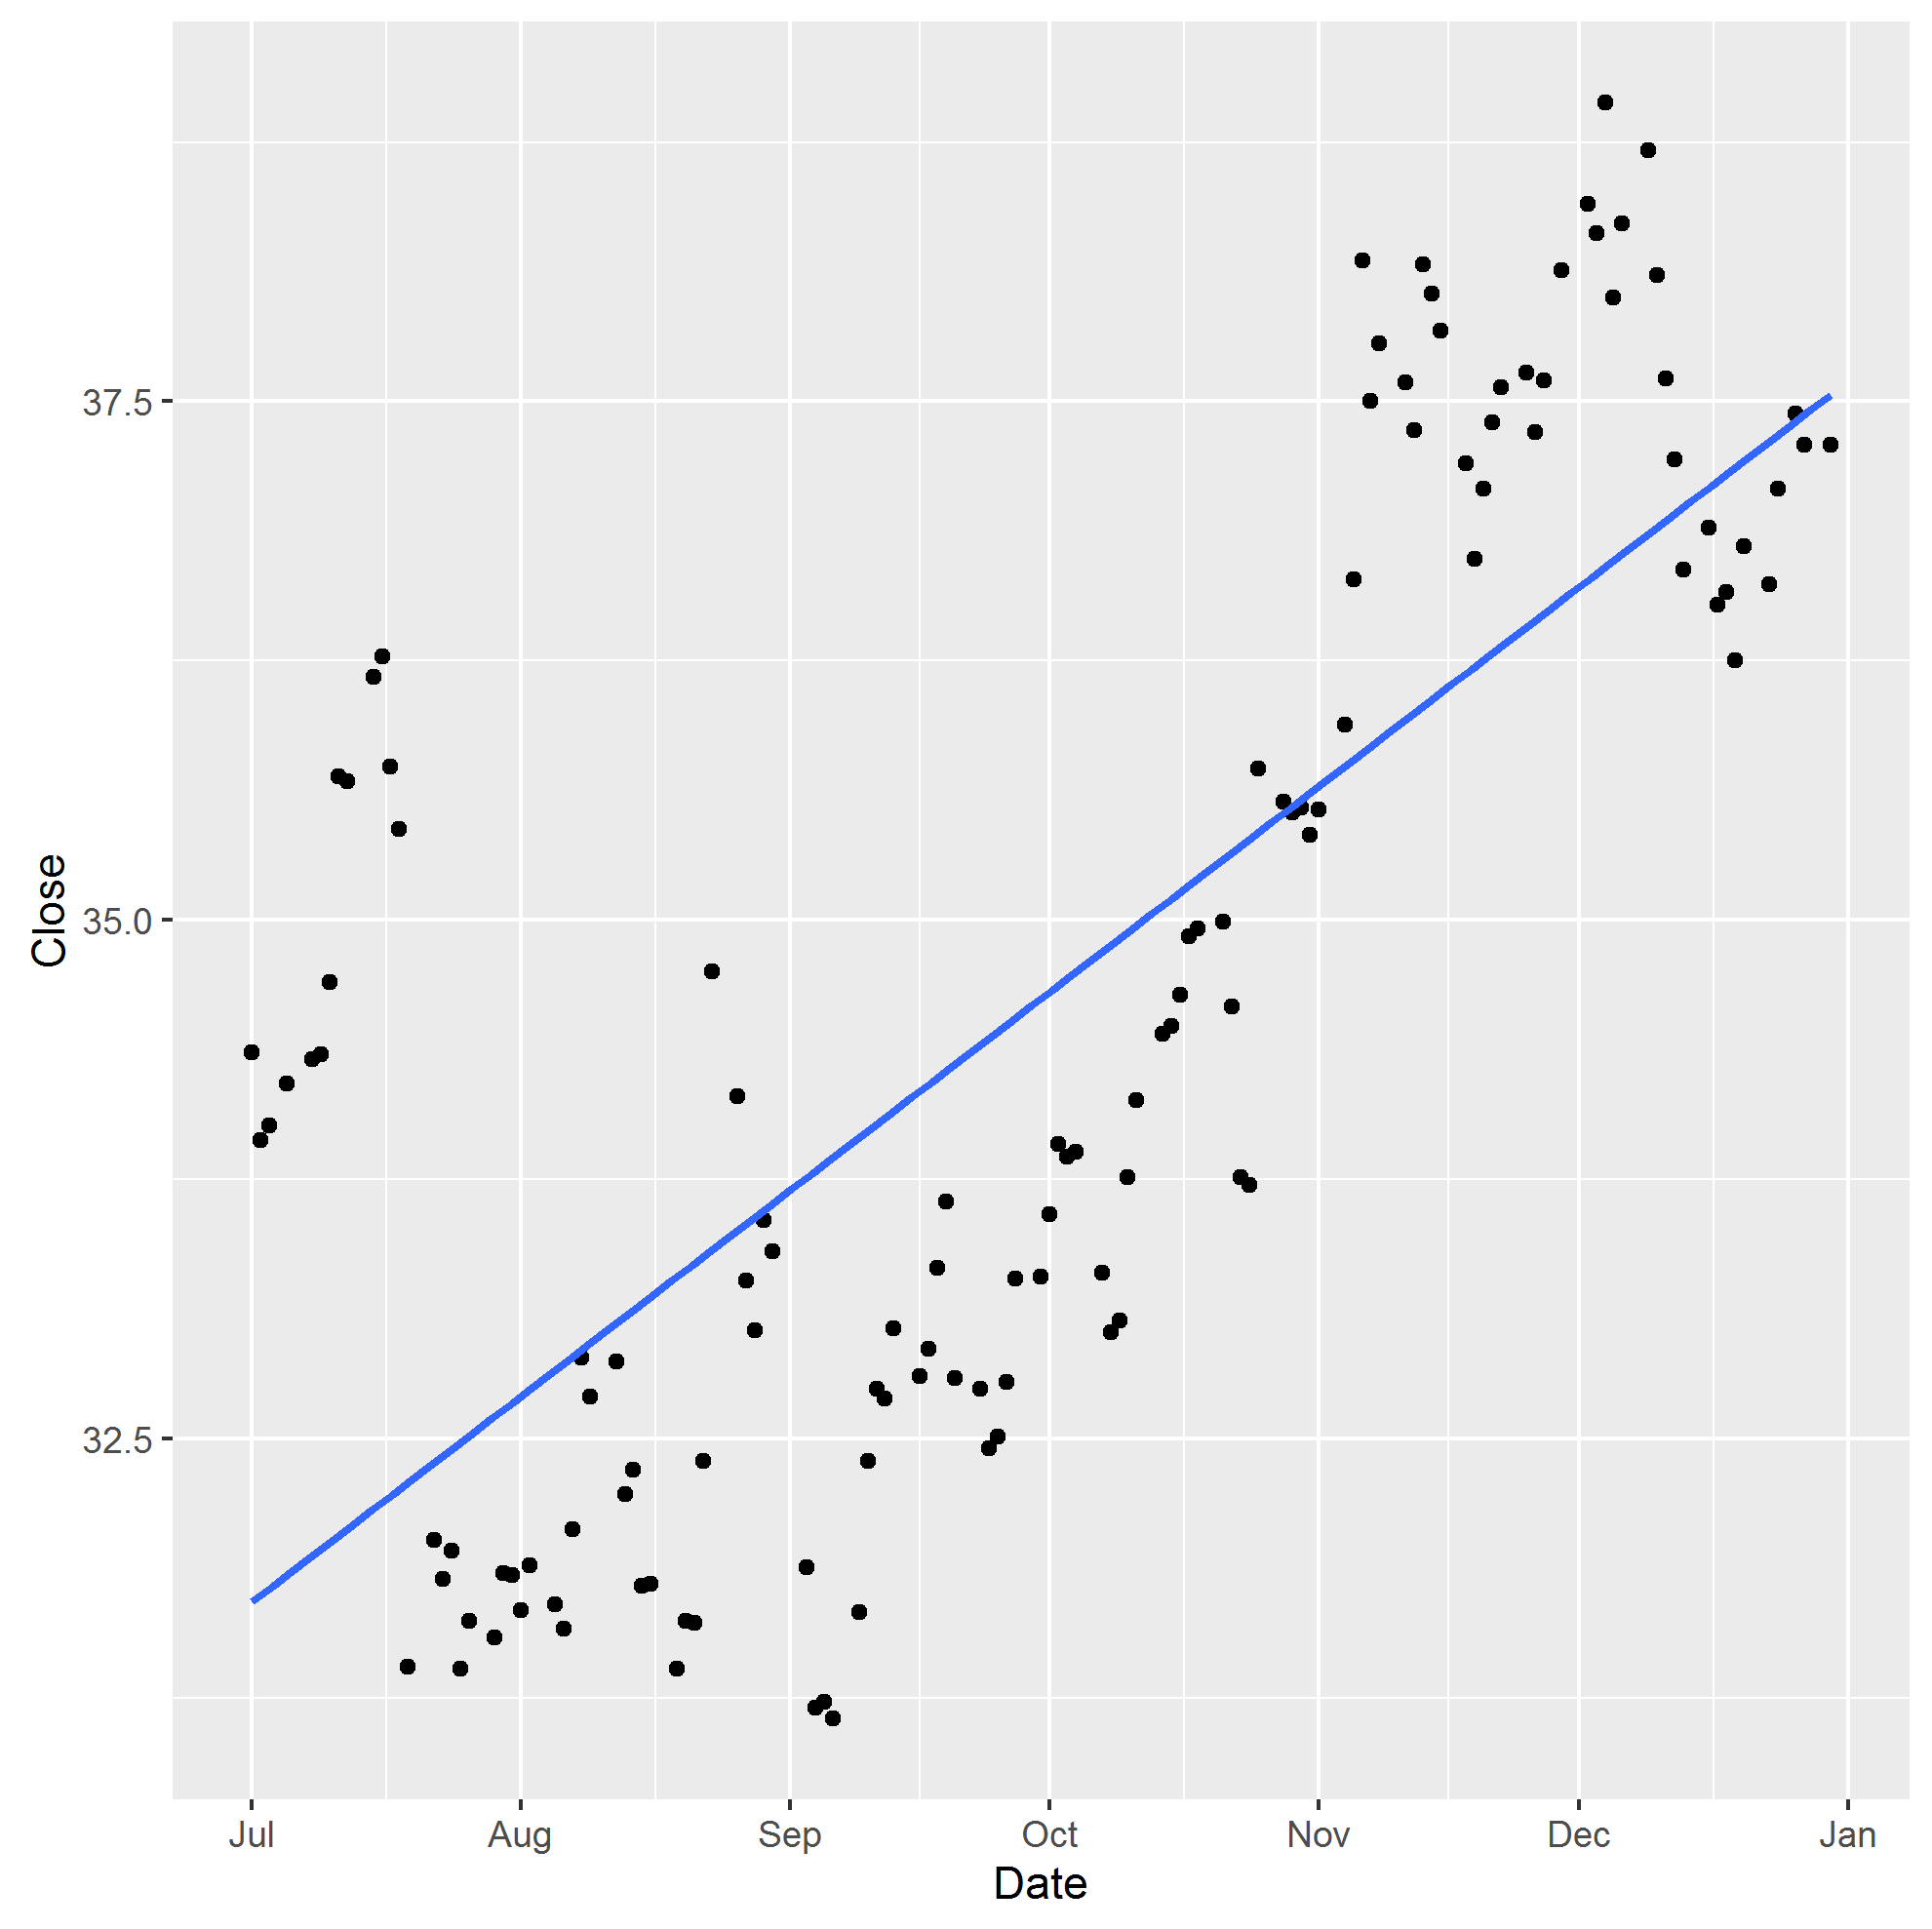
\includegraphics[width=\linewidth]{graph/m_reg6.png}
  \caption{Linear regression line of Microsoft closing prices.}
\endminipage\hfill
\end{figure}

Discuss regression lines. 

List y intercept, slope overall. 

\begin{figure}[!htb]
\minipage{0.46\textwidth}
  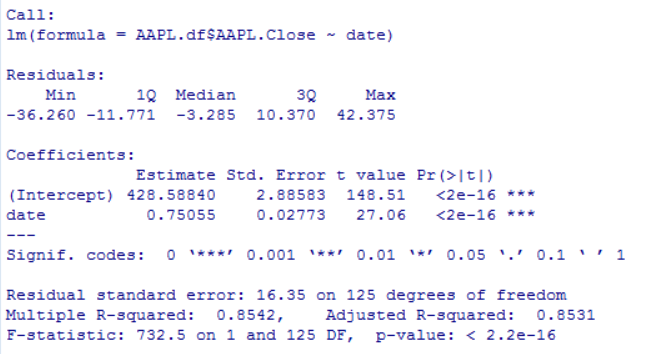
\includegraphics[width=\linewidth]{graph/aapl_reg_6.png}
  \caption{Linear regression line of Apple closing prices.}
\endminipage\hfill
\minipage{0.46\textwidth}
  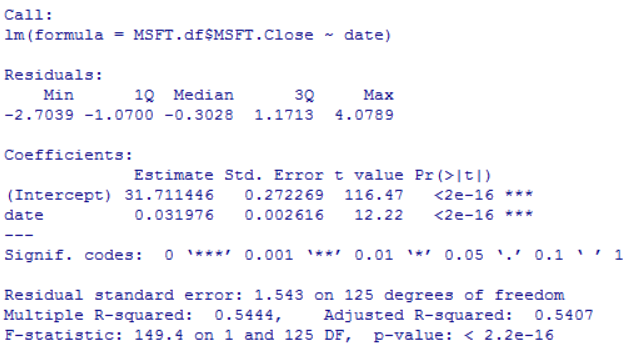
\includegraphics[width=\linewidth]{graph/msft_reg_6.png}
  \caption{Linear regression line of Microsoft closing prices.}
\endminipage\hfill
\end{figure}



\subsubsection{Analysis}
Discuss any interesting overall observations here

\subsection{January - June  2014 }
\subsubsection{Plots}
\begin{figure}[!htb]
\minipage{0.46\textwidth}
  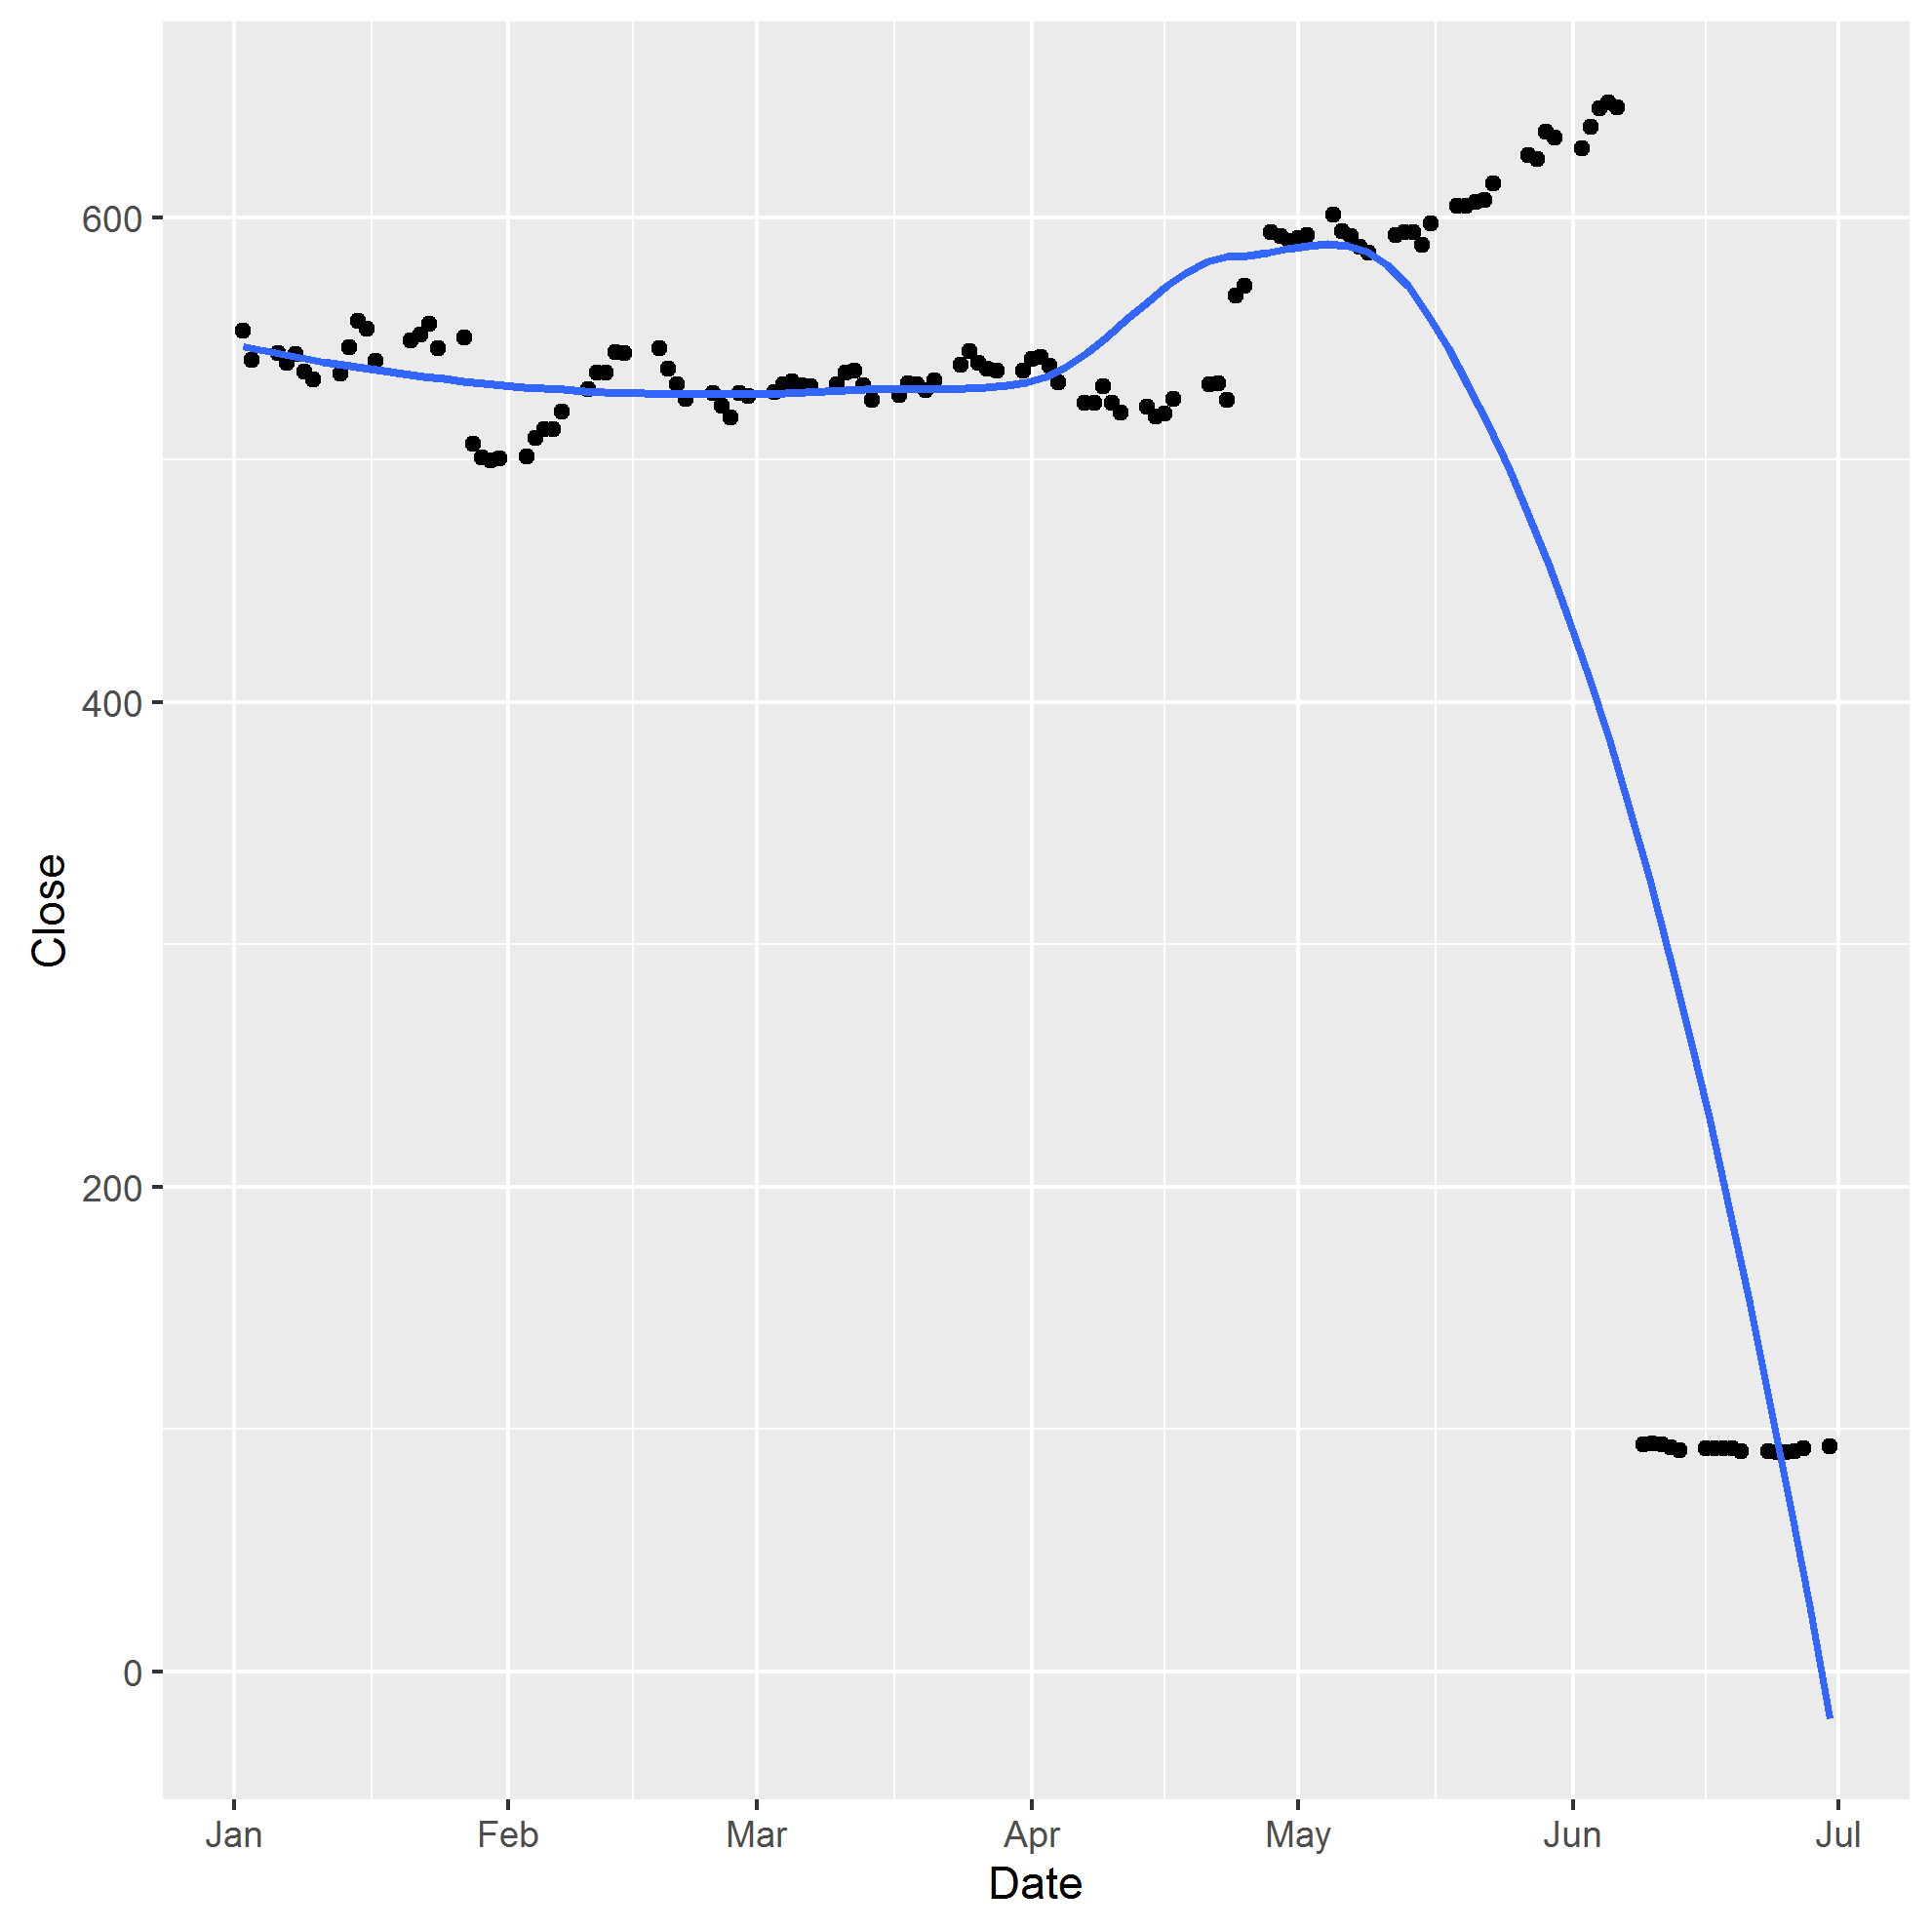
\includegraphics[width=\linewidth]{graph/AAPL7.png}
  \caption{Scatter plot with graph of Apple stock}
\endminipage\hfill
\minipage{0.46\textwidth}
  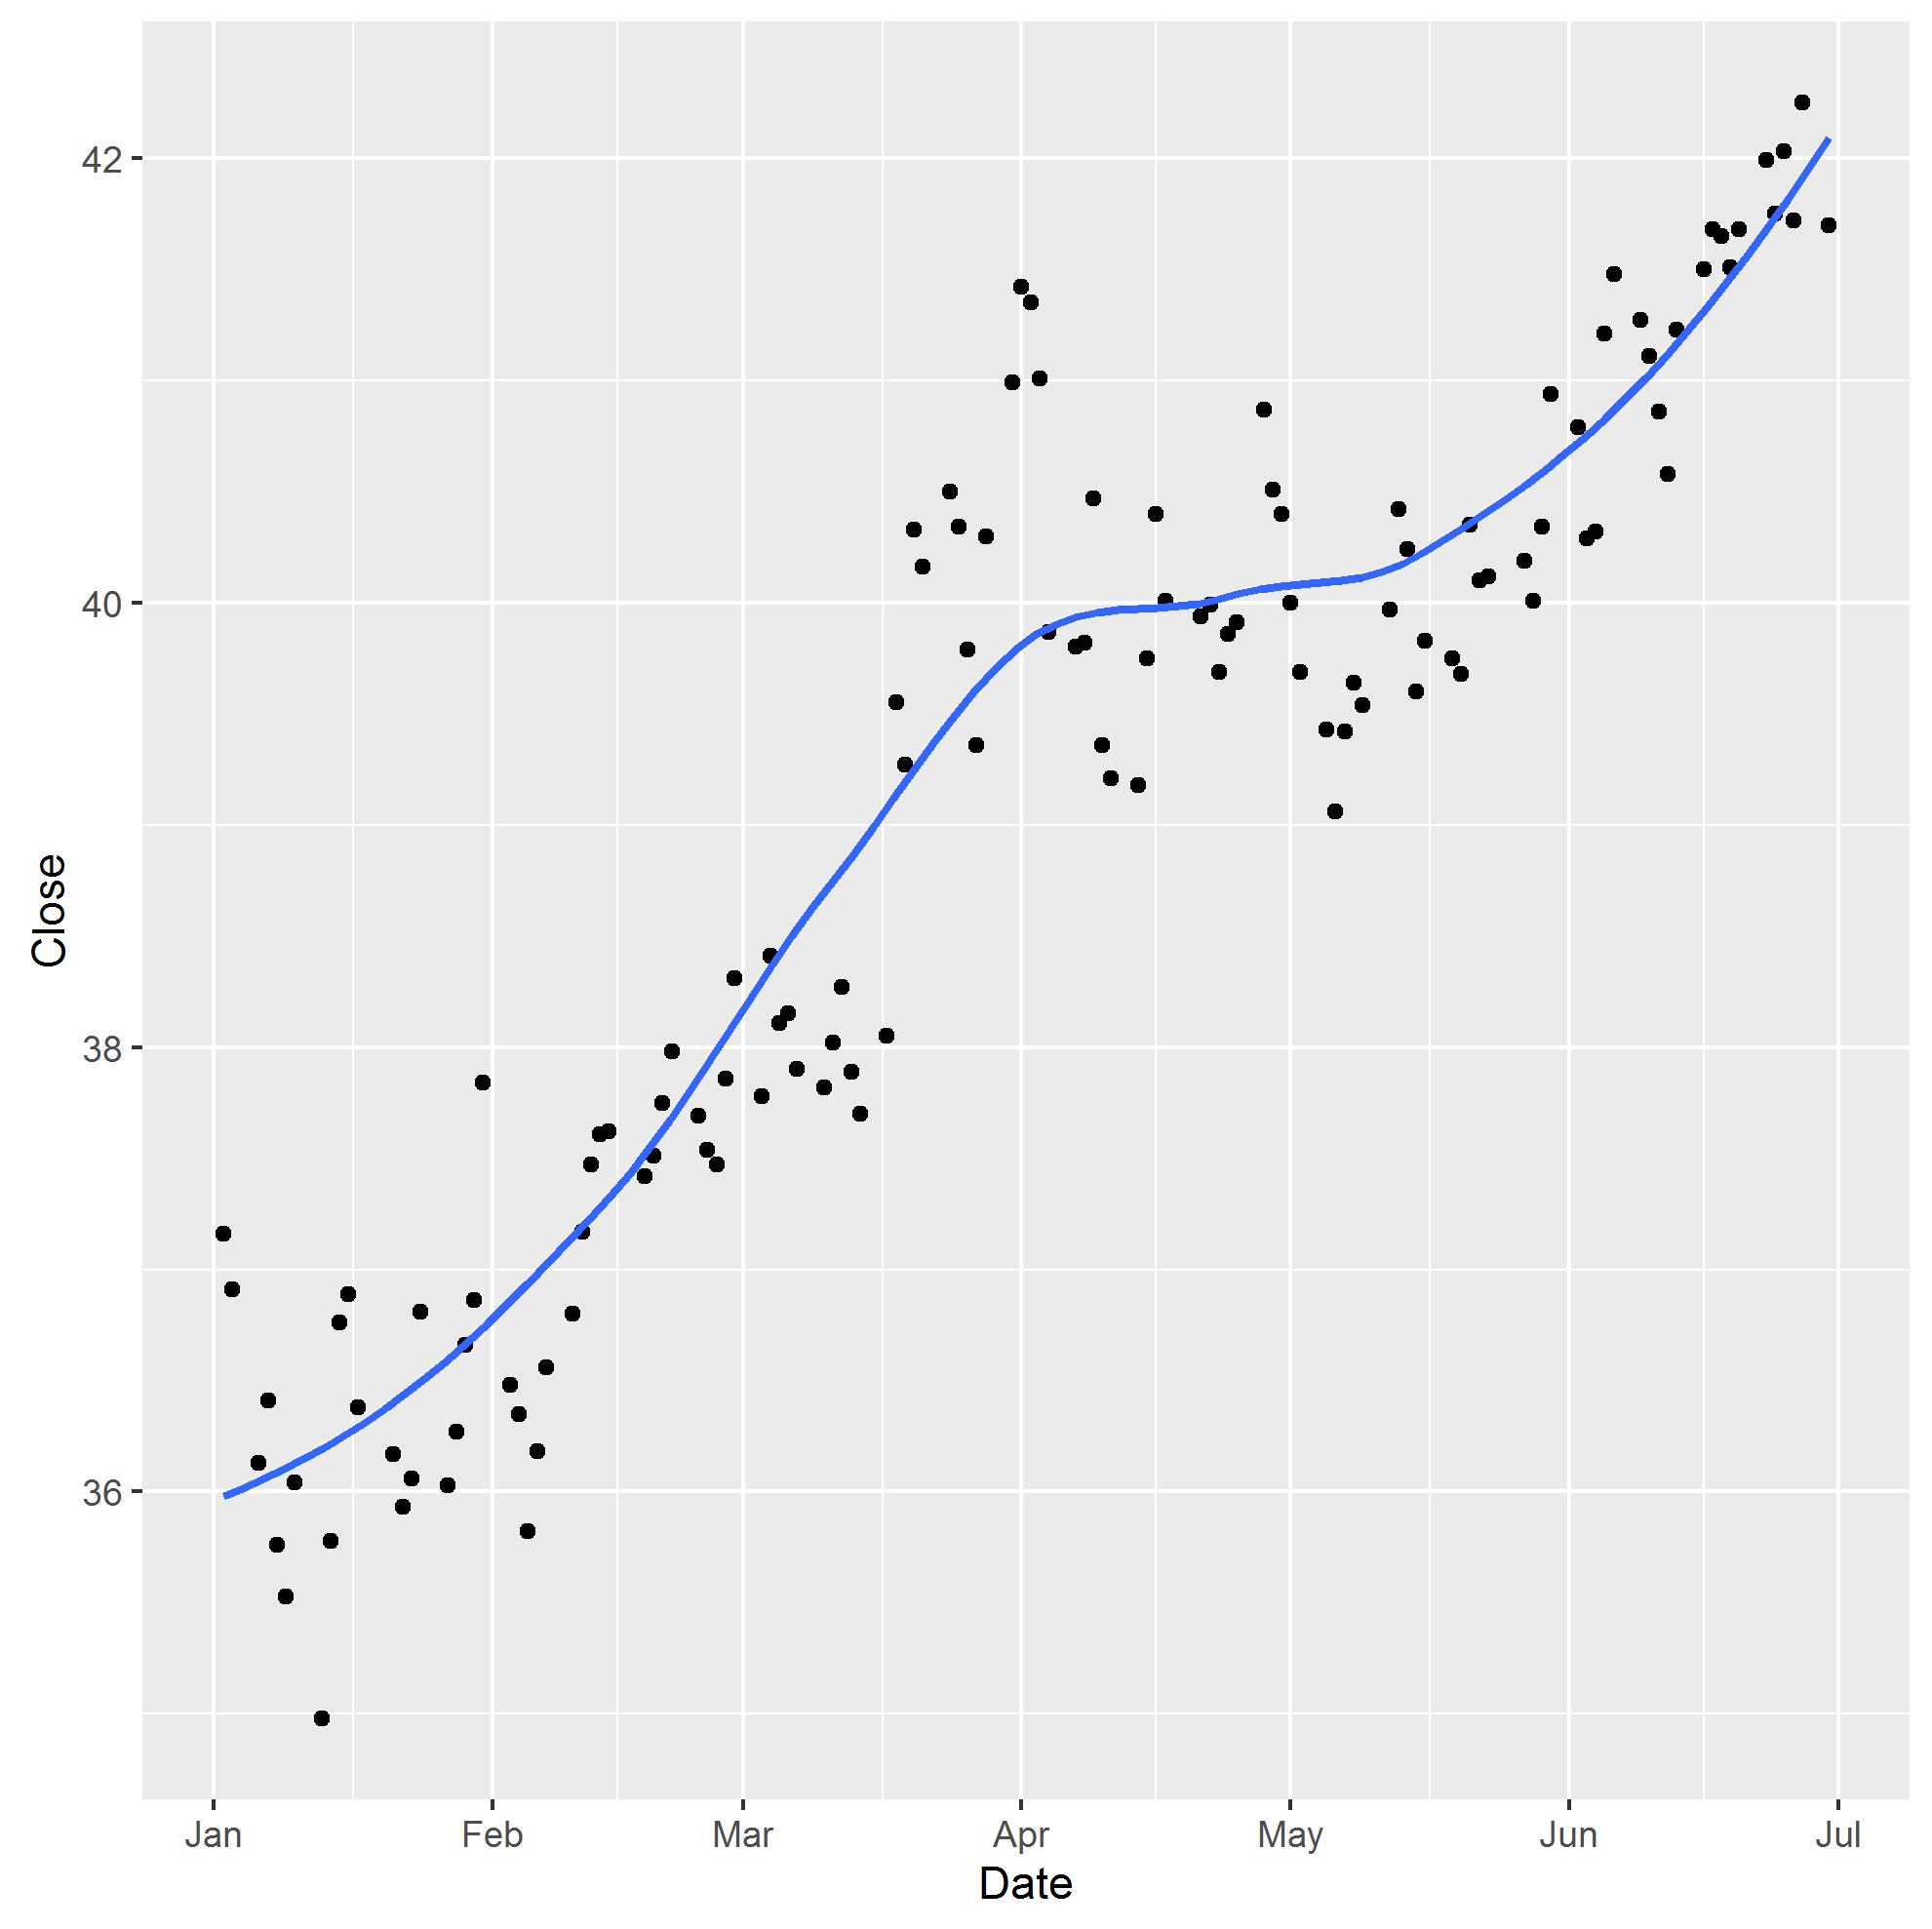
\includegraphics[width=\linewidth]{graph/MSFT7.png}
  \caption{Scatter plot with graph of Microsoft stock}
\endminipage\hfill

\end{figure}
Discuss apple chart
Discuss Microsoft chart
\subsubsection{Correlation}

\begin{figure}[!htb]
\minipage{0.8\textwidth}
  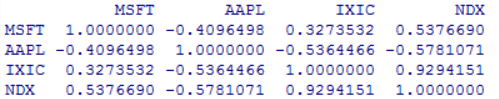
\includegraphics[width=\linewidth]{graph/cor7.png}
  \caption{Correlation table for Microsoft and Apple against two index stocks}
\endminipage\hfill
\end{figure}

Insert correlation table MS vs apple
Discuss any interesting overall observations here

\subsubsection{Regression}
Show regression lines for MS and apple. 


\begin{figure}[!htb]
\minipage{0.46\textwidth}
  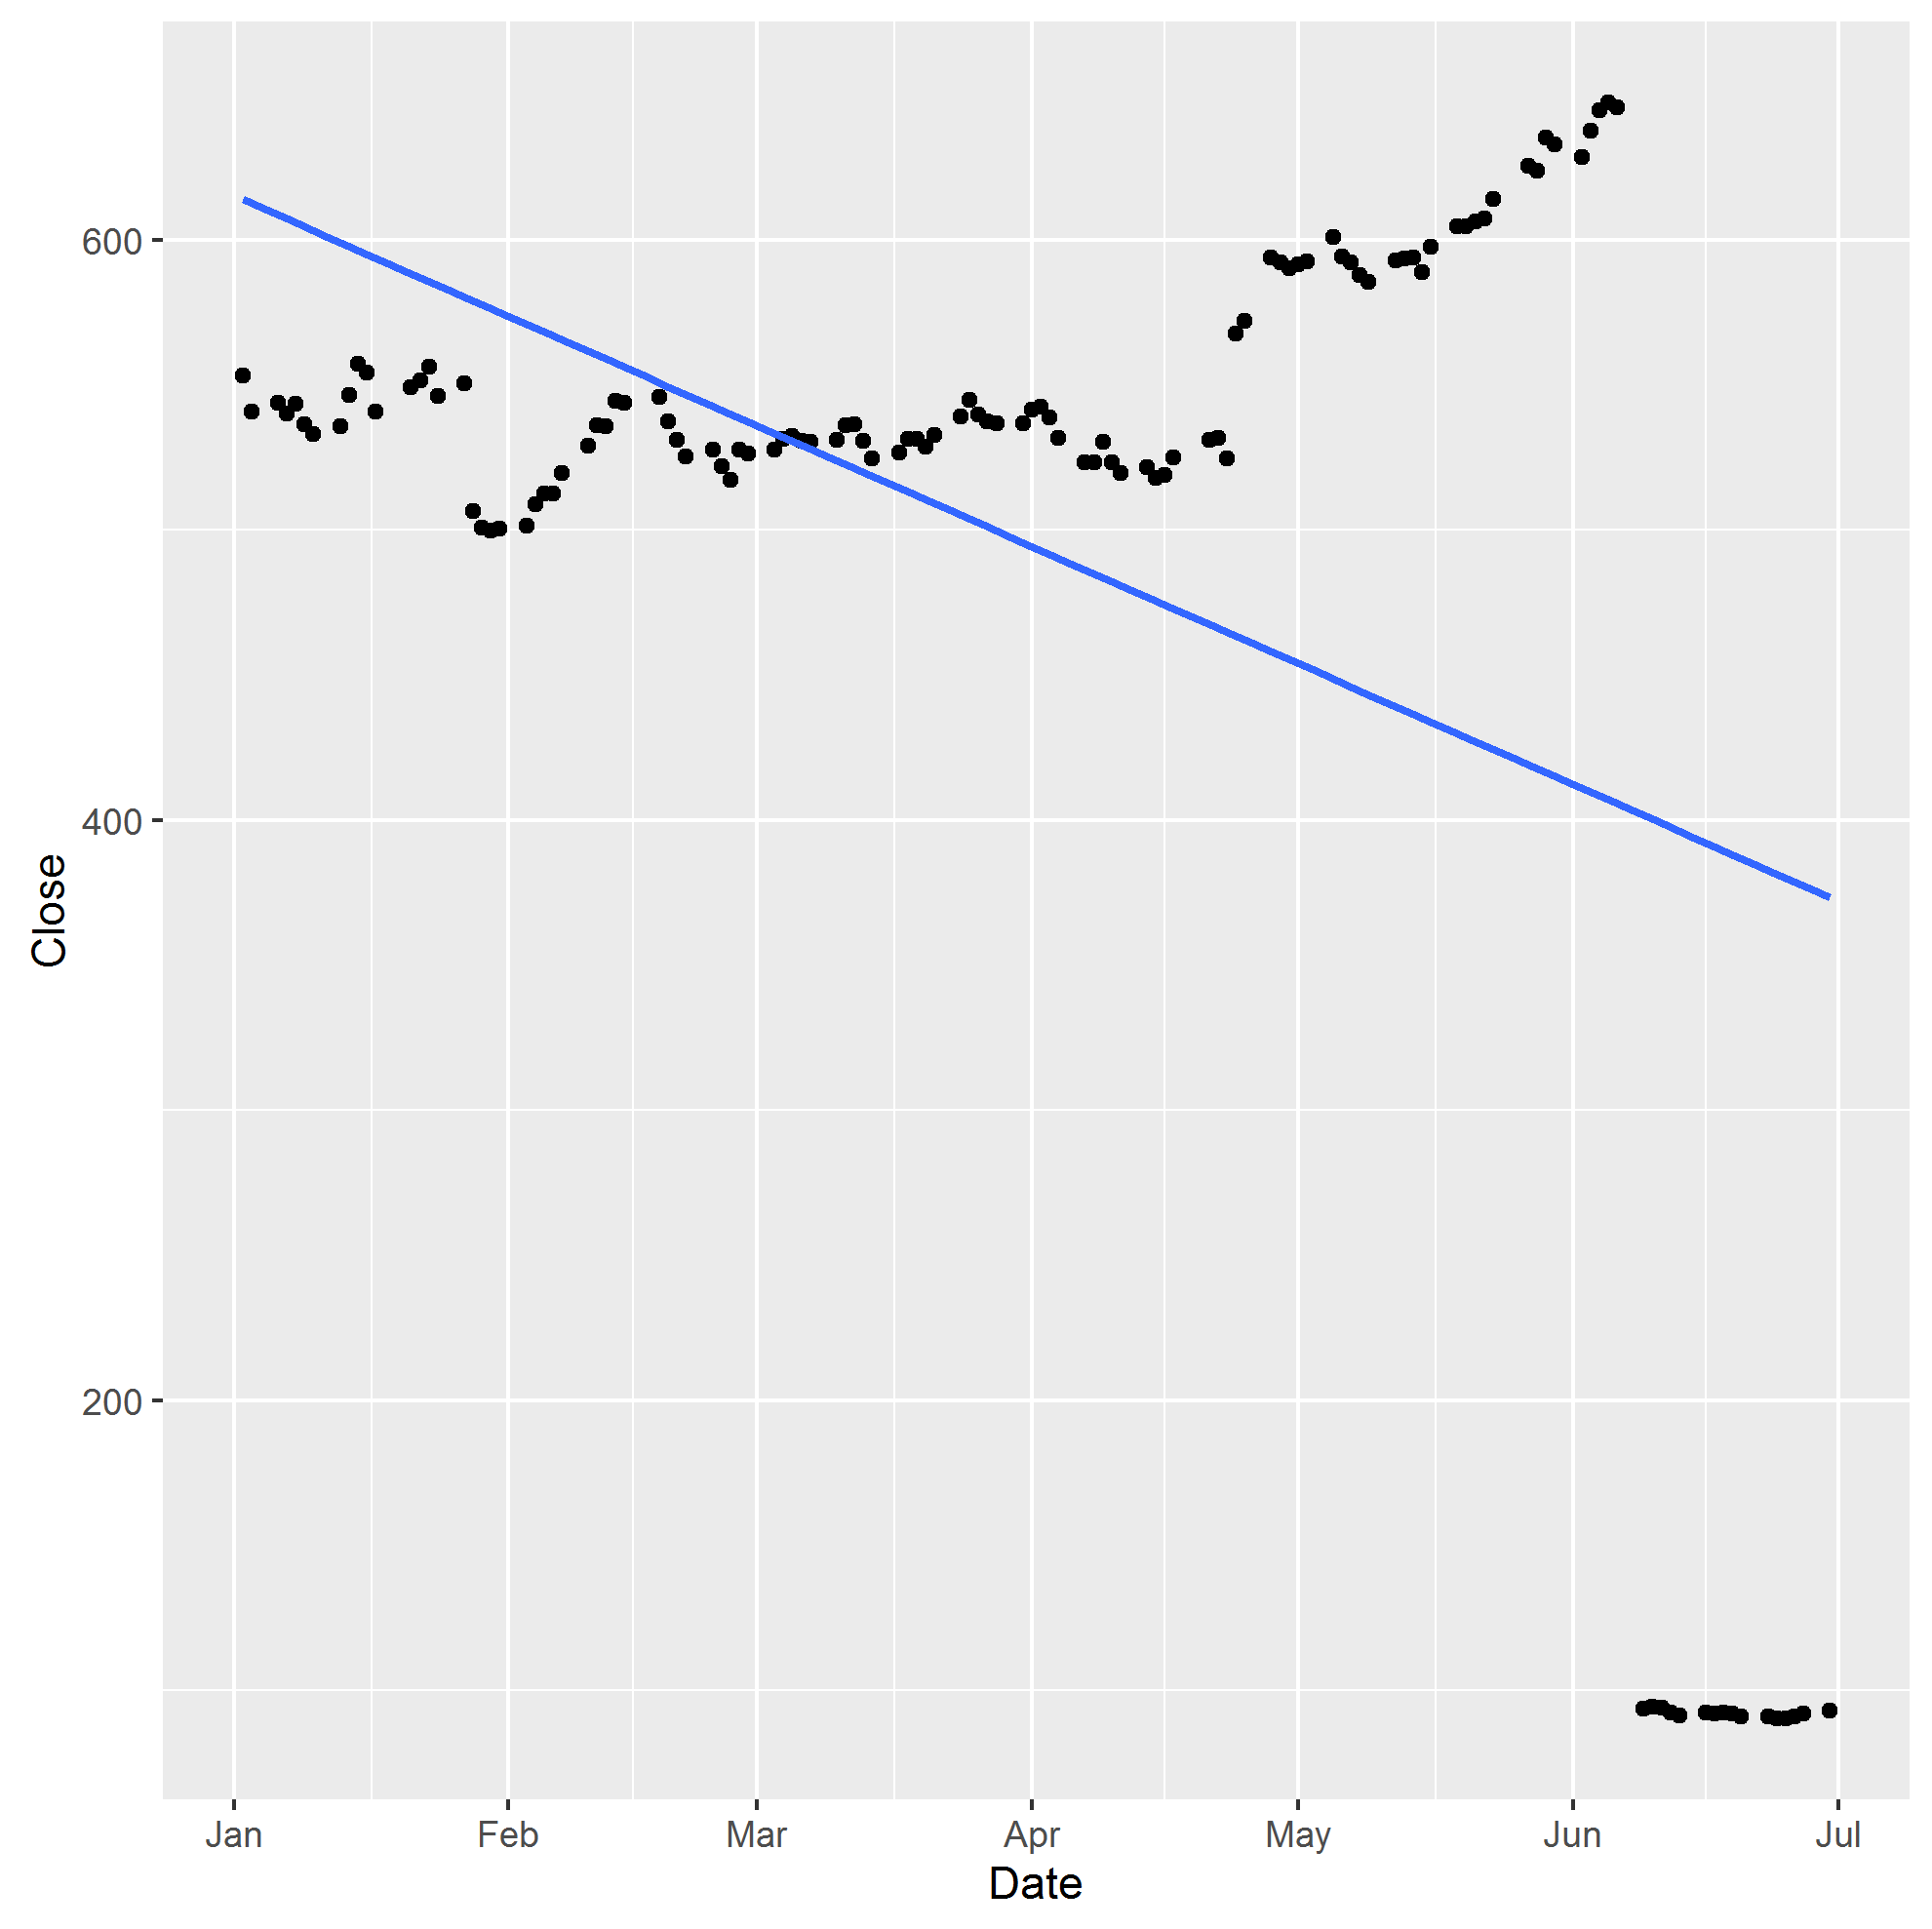
\includegraphics[width=\linewidth]{graph/a_reg7.png}
  \caption{Linear regression line of Apple closing prices.}
\endminipage\hfill
\minipage{0.46\textwidth}
  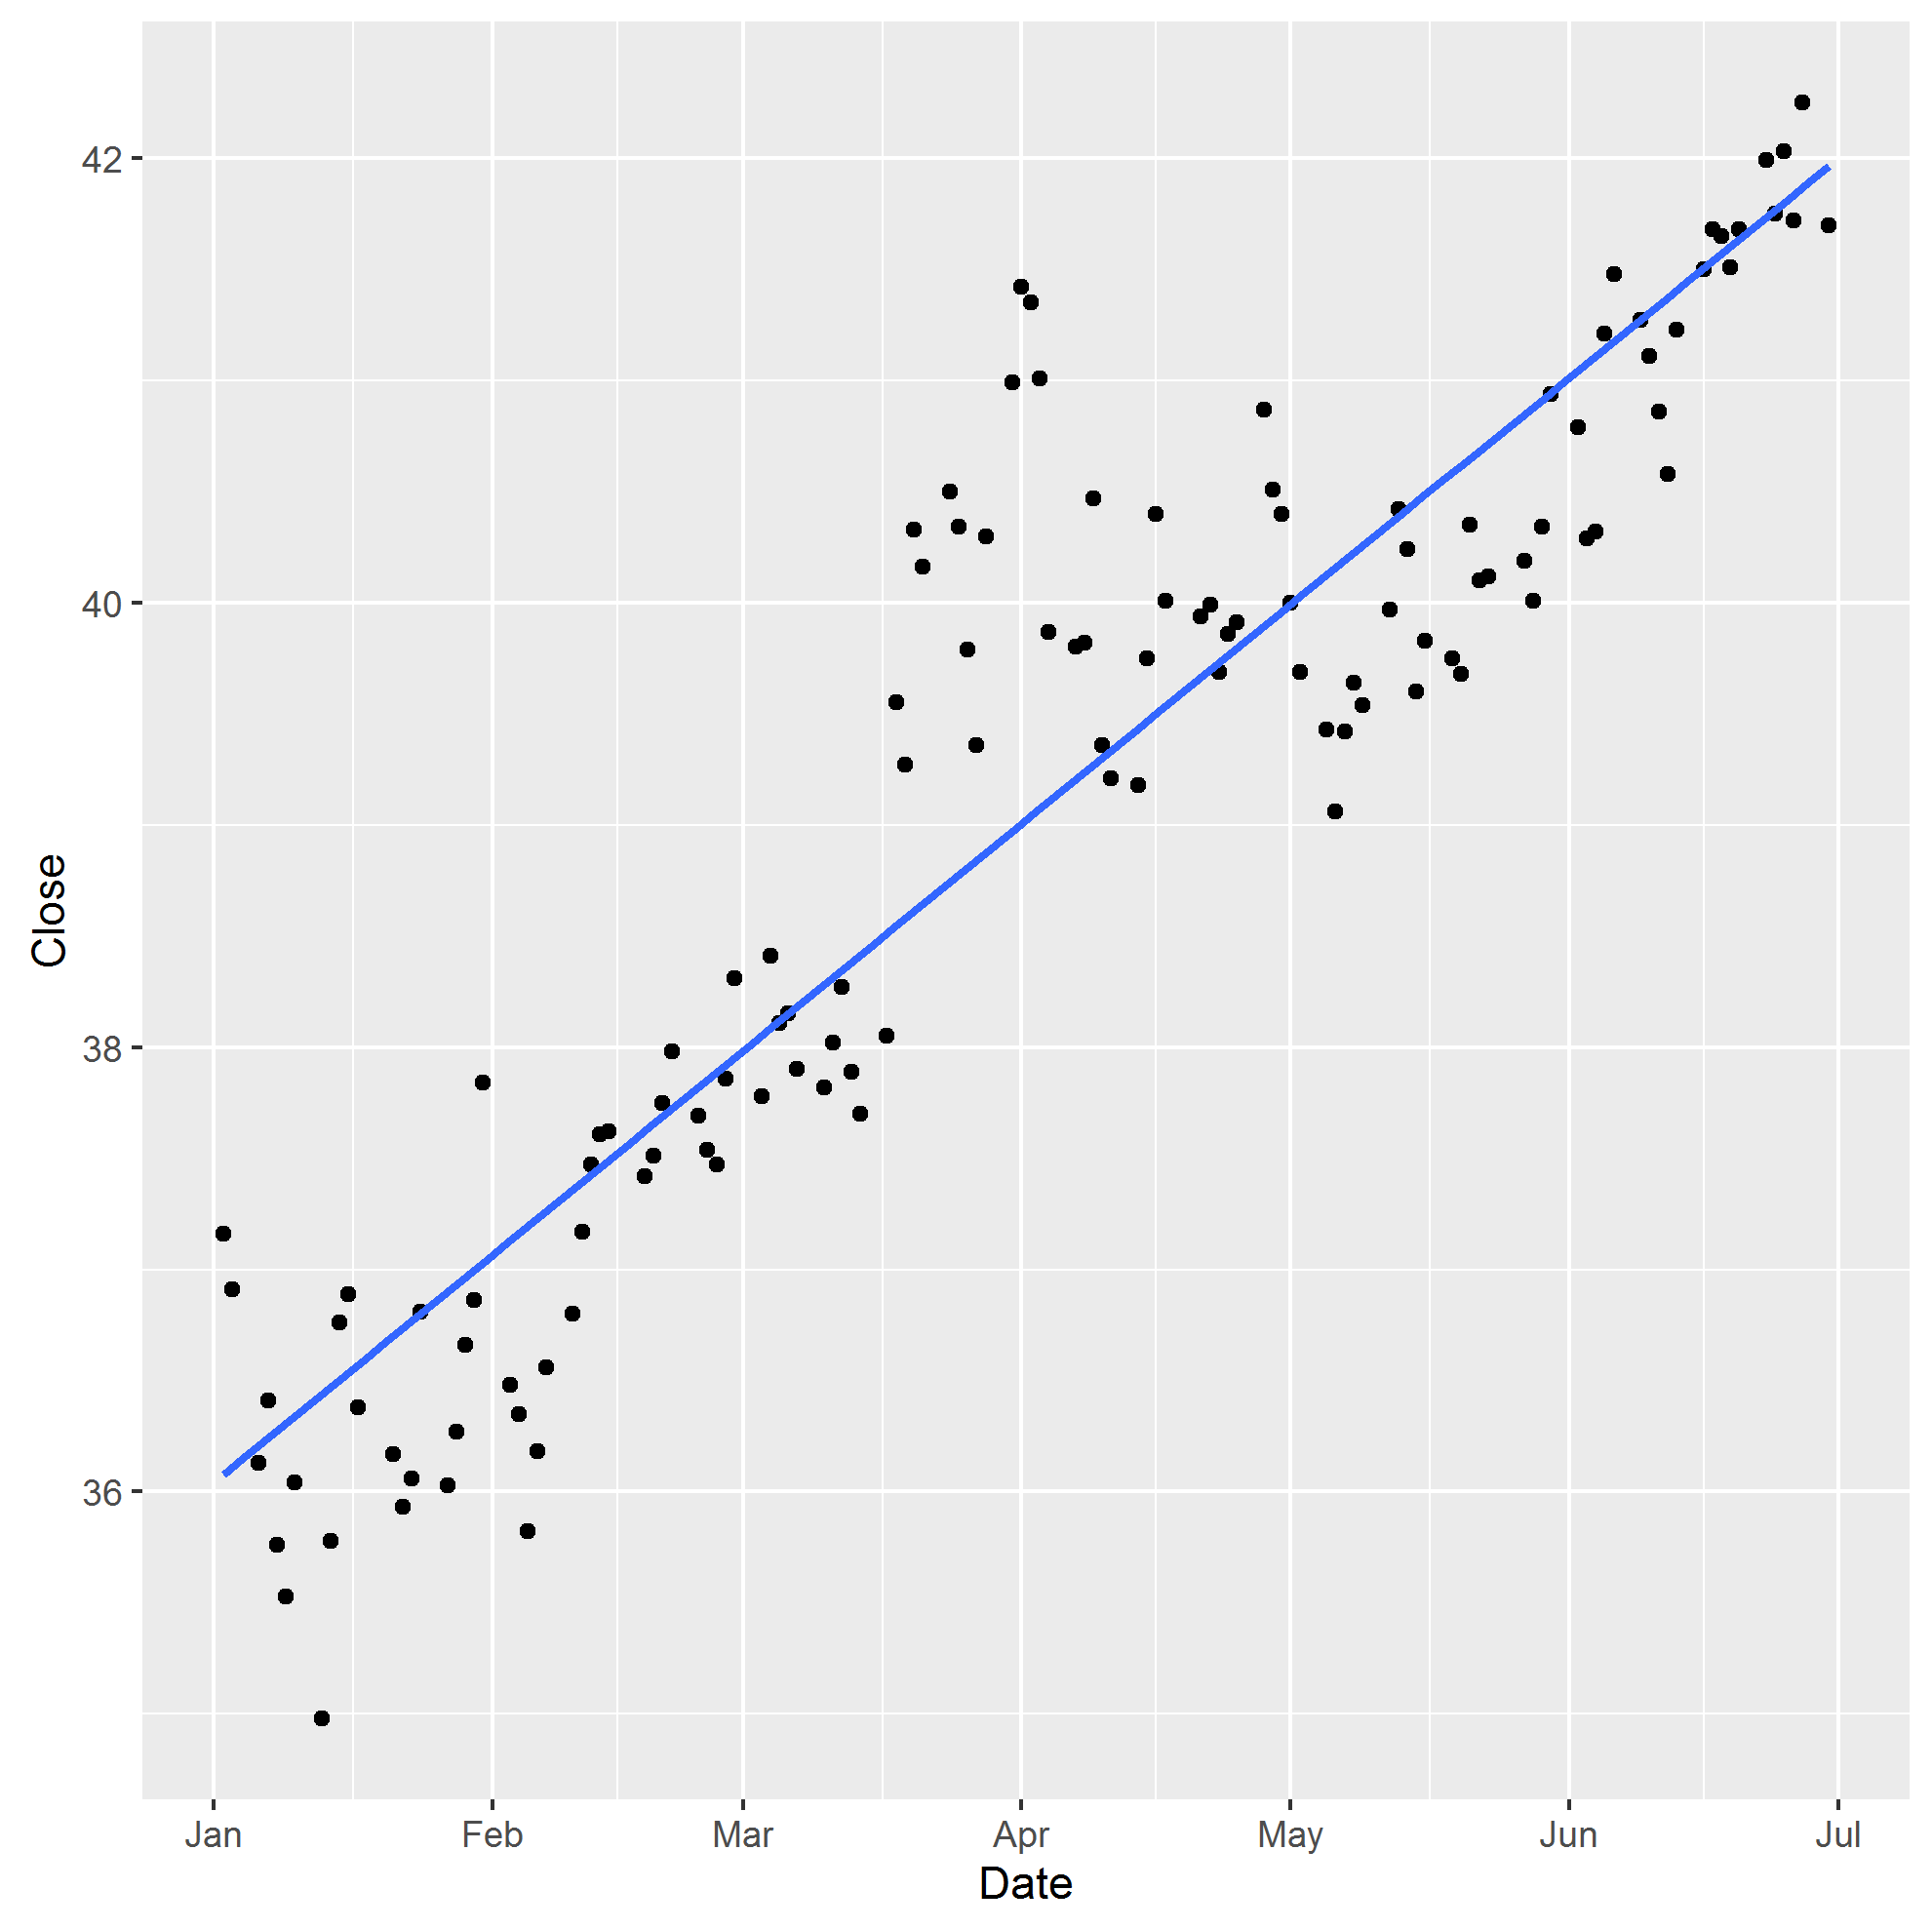
\includegraphics[width=\linewidth]{graph/m_reg7.png}
  \caption{Linear regression line of Microsoft closing prices.}
\endminipage\hfill
\end{figure}

Discuss regression lines. 

List y intercept, slope overall. 

\begin{figure}[!htb]
\minipage{0.46\textwidth}
  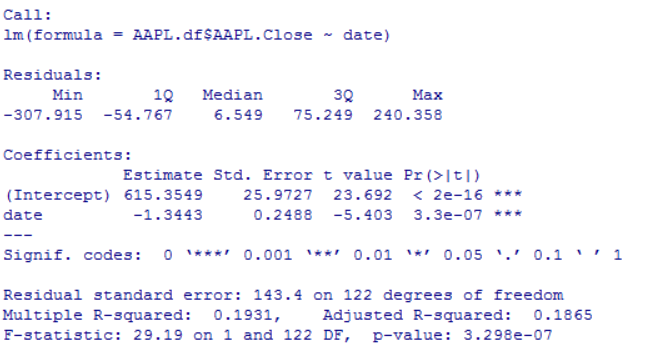
\includegraphics[width=\linewidth]{graph/aapl_reg_7.png}
  \caption{Linear regression line of Apple closing prices.}
\endminipage\hfill
\minipage{0.46\textwidth}
  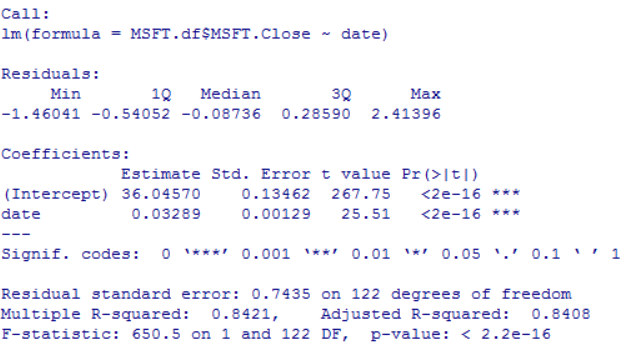
\includegraphics[width=\linewidth]{graph/msft_reg_7.png}
  \caption{Linear regression line of Microsoft closing prices.}
\endminipage\hfill
\end{figure}


\subsubsection{Analysis}
Discuss any interesting overall observations here

Discuss any interesting overall observations here

\subsection{July - December  2014}
\subsubsection{Plots}
\begin{figure}[!htb]
\minipage{0.46\textwidth}
  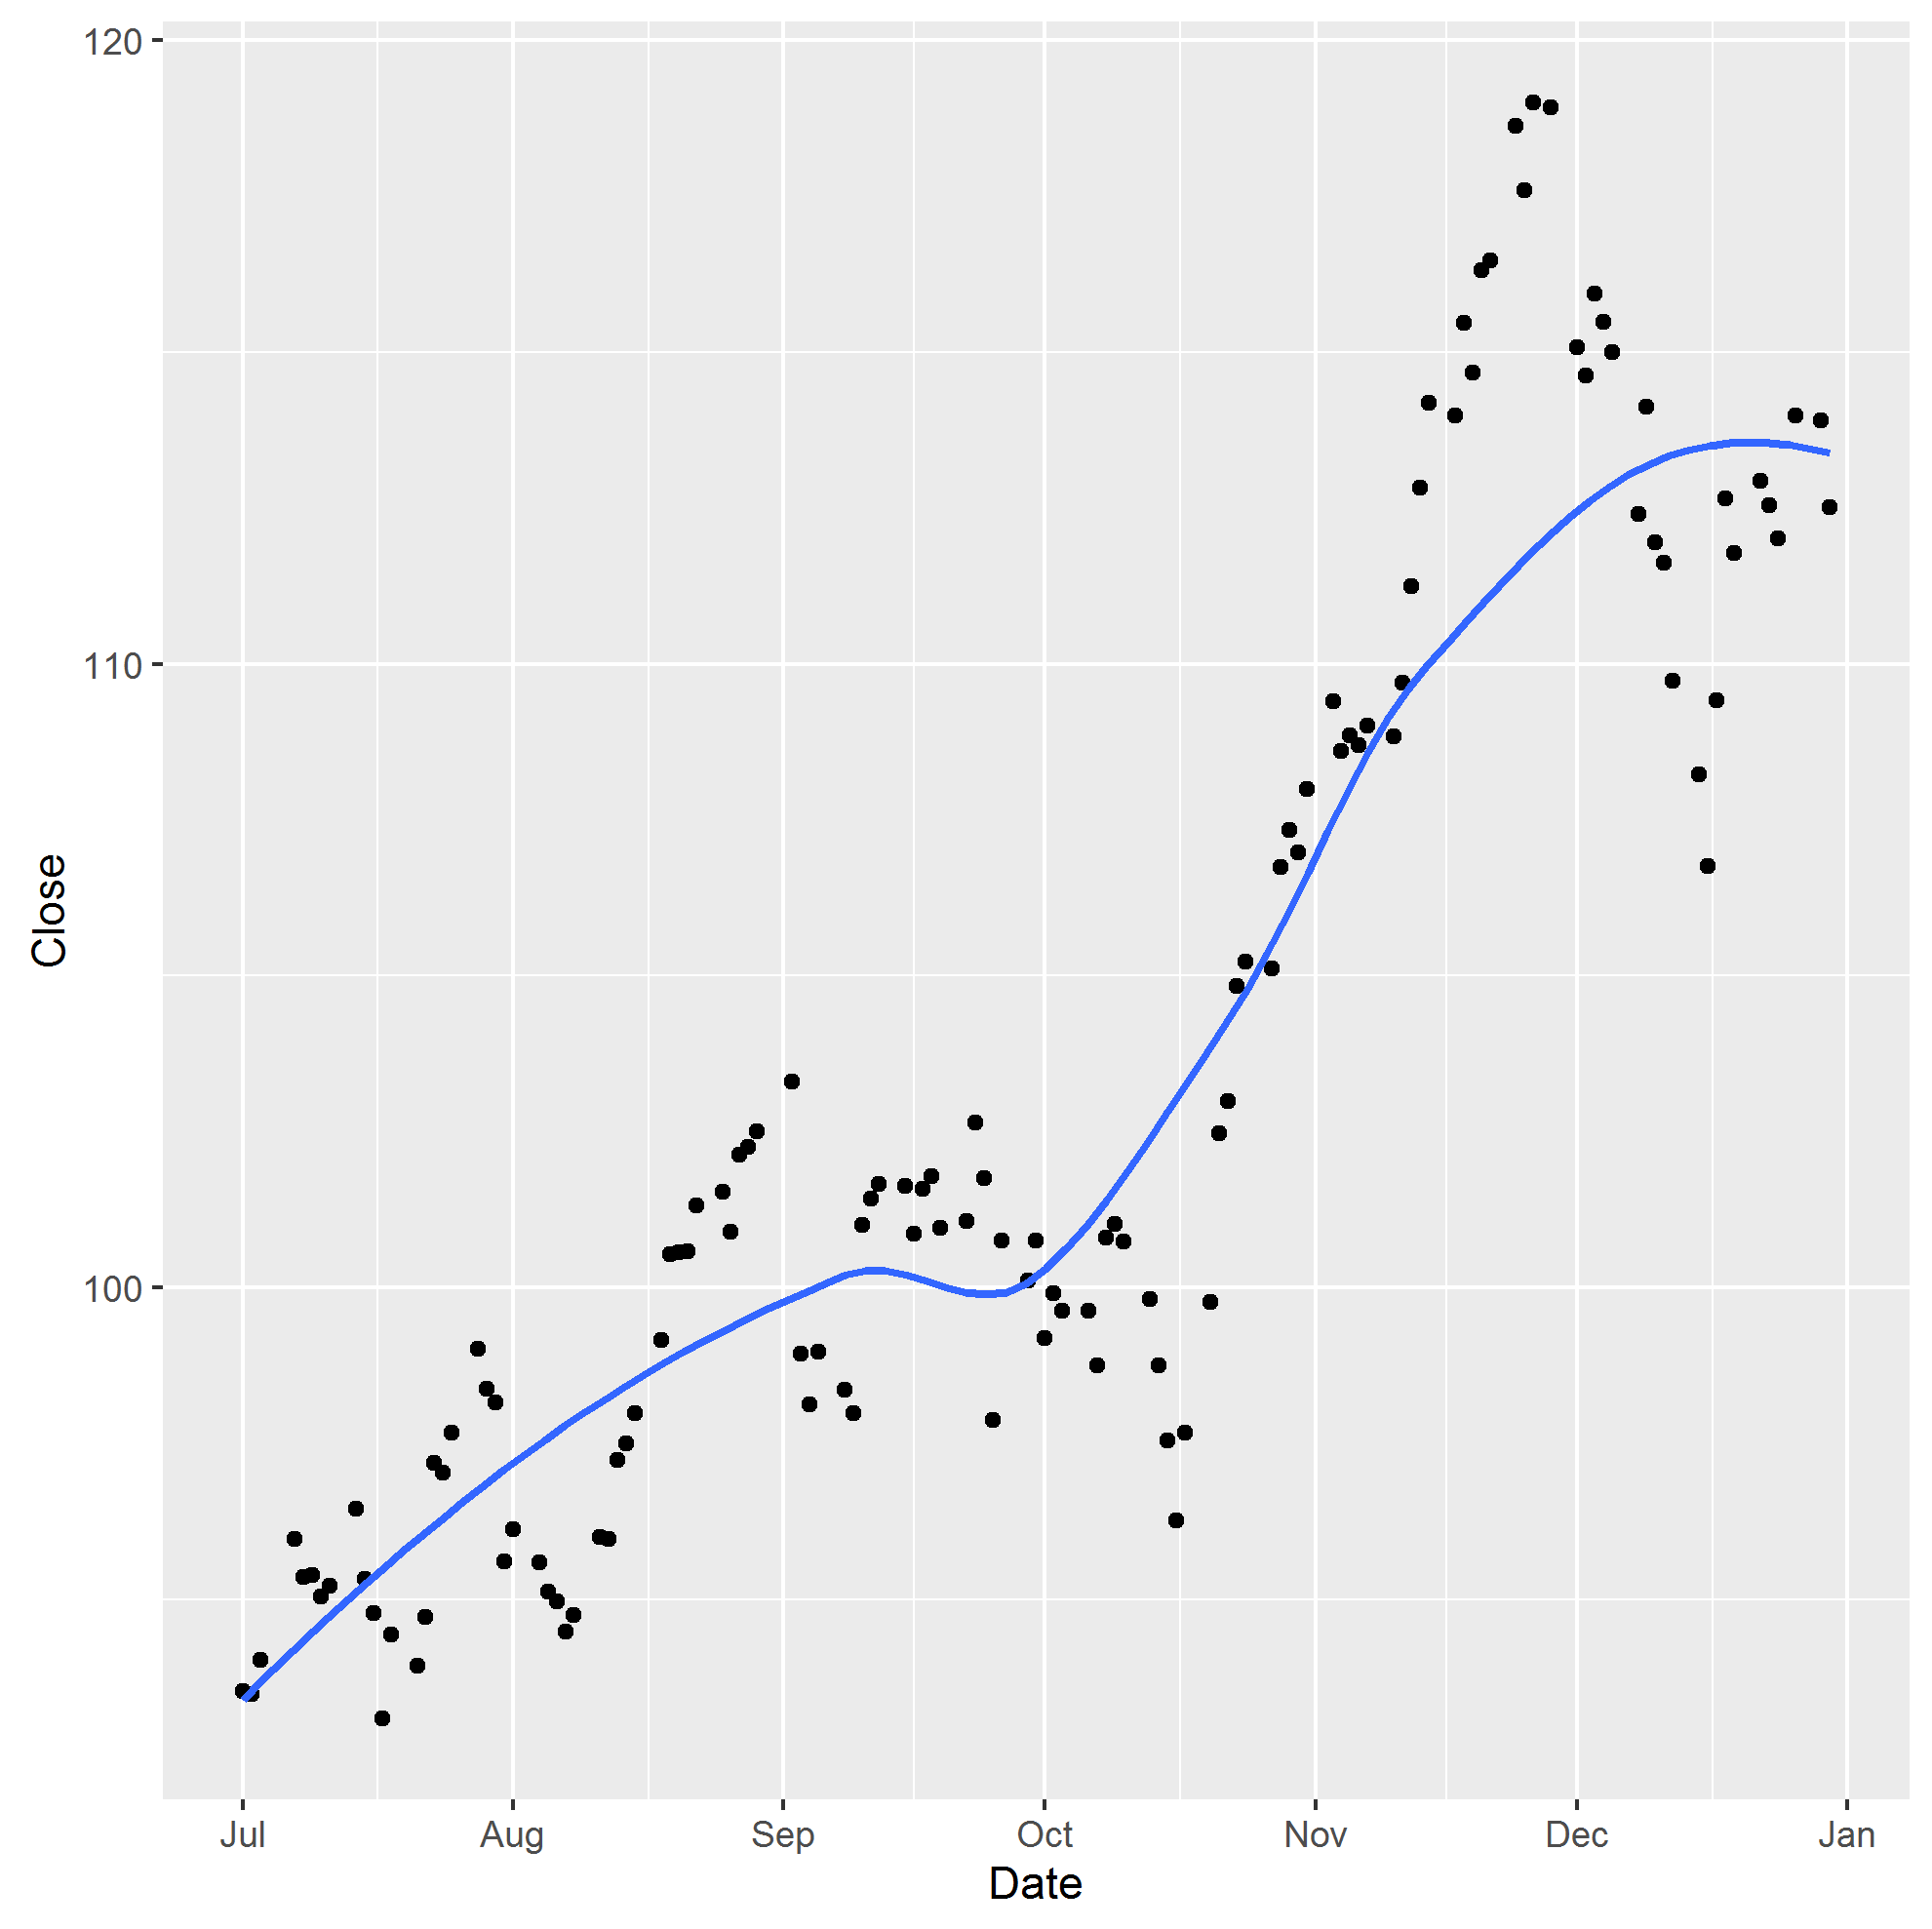
\includegraphics[width=\linewidth]{graph/AAPL8.png}
  \caption{Scatter plot with graph of Apple stock}
\endminipage\hfill
\minipage{0.46\textwidth}
  \includegraphics[width=\linewidth]{graph/MSFT8.png}
  \caption{Scatter plot with graph of Microsoft stock}
\endminipage\hfill

\end{figure}
Discuss apple chart
Discuss Microsoft chart
\subsubsection{Correlation}

\begin{figure}[!htb]
\minipage{0.8\textwidth}
  \includegraphics[width=\linewidth]{graph/cor8.png}
  \caption{Correlation table for Microsoft and Apple against two index stocks}
\endminipage\hfill
\end{figure}

Insert correlation table MS vs apple
Discuss any interesting overall observations here

\subsubsection{Regression}
Show regression lines for MS and apple. 


\begin{figure}[!htb]
\minipage{0.46\textwidth}
  \includegraphics[width=\linewidth]{graph/a_reg8.png}
  \caption{Linear regression line of Apple closing prices.}
\endminipage\hfill
\minipage{0.46\textwidth}
  \includegraphics[width=\linewidth]{graph/m_reg8.png}
  \caption{Linear regression line of Microsoft closing prices.}
\endminipage\hfill
\end{figure}

Discuss regression lines. 

List y intercept, slope overall. 

\begin{figure}[!htb]
\minipage{0.46\textwidth}
  \includegraphics[width=\linewidth]{graph/aapl_reg_8.png}
  \caption{Linear regression line of Apple closing prices.}
\endminipage\hfill
\minipage{0.46\textwidth}
  \includegraphics[width=\linewidth]{graph/msft_reg_8.png}
  \caption{Linear regression line of Microsoft closing prices.}
\endminipage\hfill
\end{figure}


\subsubsection{Analysis}
Discuss any interesting overall observations here

Discuss any interesting overall observations here

\subsection{January - June  2015 }
\subsubsection{Plots}
\begin{figure}[!htb]
\minipage{0.46\textwidth}
  \includegraphics[width=\linewidth]{graph/AAPL9.png}
  \caption{Scatter plot with graph of Apple stock}
\endminipage\hfill
\minipage{0.46\textwidth}
  \includegraphics[width=\linewidth]{graph/MSFT9.png}
  \caption{Scatter plot with graph of Microsoft stock}
\endminipage\hfill

\end{figure}
Discuss apple chart
Discuss Microsoft chart
\subsubsection{Correlation}

\begin{figure}[!htb]
\minipage{0.8\textwidth}
  \includegraphics[width=\linewidth]{graph/cor9.png}
  \caption{Correlation table for Microsoft and Apple against two index stocks}
\endminipage\hfill
\end{figure}

Insert correlation table MS vs apple
Discuss any interesting overall observations here

\subsubsection{Regression}
Show regression lines for MS and apple. 


\begin{figure}[!htb]
\minipage{0.46\textwidth}
  \includegraphics[width=\linewidth]{graph/a_reg9.png}
  \caption{Linear regression line of Apple closing prices.}
\endminipage\hfill
\minipage{0.46\textwidth}
  \includegraphics[width=\linewidth]{graph/m_reg9.png}
  \caption{Linear regression line of Microsoft closing prices.}
\endminipage\hfill
\end{figure}

Discuss regression lines. 

List y intercept, slope overall. 

\begin{figure}[!htb]
\minipage{0.46\textwidth}
  \includegraphics[width=\linewidth]{graph/aapl_reg_9.png}
  \caption{Linear regression line of Apple closing prices.}
\endminipage\hfill
\minipage{0.46\textwidth}
  \includegraphics[width=\linewidth]{graph/msft_reg_9.png}
  \caption{Linear regression line of Microsoft closing prices.}
\endminipage\hfill
\end{figure}


\subsubsection{Analysis}
Discuss any interesting overall observations here


\subsection{July - December  2015}
\subsubsection{Plots}
\begin{figure}[!htb]
\minipage{0.46\textwidth}
  \includegraphics[width=\linewidth]{graph/AAPL10.png}
  \caption{Scatter plot with graph of Apple stock}
\endminipage\hfill
\minipage{0.46\textwidth}
  \includegraphics[width=\linewidth]{graph/MSFT10.png}
  \caption{Scatter plot with graph of Microsoft stock}
\endminipage\hfill

\end{figure}
Discuss apple chart
Discuss Microsoft chart
\subsubsection{Correlation}

\begin{figure}[!htb]
\minipage{0.8\textwidth}
  \includegraphics[width=\linewidth]{graph/cor10.png}
  \caption{Correlation table for Microsoft and Apple against two index stocks}
\endminipage\hfill
\end{figure}

Insert correlation table MS vs apple
Discuss any interesting overall observations here

\subsubsection{Regression}
Show regression lines for MS and apple. 


\begin{figure}[!htb]
\minipage{0.46\textwidth}
  \includegraphics[width=\linewidth]{graph/a_reg10.png}
  \caption{Linear regression line of Apple closing prices.}
\endminipage\hfill
\minipage{0.46\textwidth}
  \includegraphics[width=\linewidth]{graph/m_reg10.png}
  \caption{Linear regression line of Microsoft closing prices.}
\endminipage\hfill
\end{figure}

Discuss regression lines. 

List y intercept, slope overall. 

\begin{figure}[!htb]
\minipage{0.46\textwidth}
  \includegraphics[width=\linewidth]{graph/aapl_reg_10.png}
  \caption{Linear regression line of Apple closing prices.}
\endminipage\hfill
\minipage{0.46\textwidth}
  \includegraphics[width=\linewidth]{graph/msft_reg_10.png}
  \caption{Linear regression line of Microsoft closing prices.}
\endminipage\hfill
\end{figure}


\subsubsection{Analysis}
Discuss any interesting overall observations here


\subsection{Forecasting and Analysis}

Describe how well the models work for the performance over the next 6 months. 

\section{Conclusions}

Discuss anything particularly interesting. 

Talk about how short term stock analysis is more likely to be useful due to stocks being similar to chaotic systems with little long term predictability. 

Discuss how linear models are not likely to be best and future work should focus on better models. 

What did we just do?


\bibliographystyle{plain}
\bibliography{finbib}

\end{document}